\documentclass[aps,onecolumn,nofootinbib,pra]{article}

\usepackage{../../article_compilation/spec_files/arxiv}
\input{../../article_compilation/spec_files/standard_preamble.tex}

% Text Macros
\newcommand{\python}{$\mathrm{python}$}
\newcommand{\tnreason}{$\mathrm{tnreason}$}
\newcommand{\qcreason}{$\mathrm{qcreason}$}

\newcommand{\spengine}{$\mathrm{engine}$}
\newcommand{\sprepresentation}{$\mathrm{representation}$}
\newcommand{\spreasoning}{$\mathrm{reasoning}$}
\newcommand{\spapplication}{$\mathrm{application}$}

\newcommand{\layeronespec}{\textbf{Layer 1}: Storage and manipulations}
\newcommand{\layertwospec}{\textbf{Layer 2}: Specification of workload}
\newcommand{\layerthreespec}{\textbf{Layer 3}: Applications in reasoning}

% Current tnreason version
\newcommand{\curvertnreason}{2.0.0}

% Report Chapters
\newcommand{\partonetext}{Foundations} % was Classical Approaches
\newcommand{\chatextprobRepresentation}{Probability Distributions}
\newcommand{\chatextprobReasoning}{Probabilistic Inference}
\newcommand{\chatextlogicalRepresentation}{Propositional Logic}
\newcommand{\chatextlogicalReasoning}{Logical Inference}

\newcommand{\parttwotext}{Hybrid Logic Networks} % was Neuro-Symbolic Applications
\newcommand{\chatextformulaSelection}{Formula Selecting Networks}
\newcommand{\chatextnetworkRepresentation}{Hybrid Logic Representation}
\newcommand{\chatextnetworkReasoning}{Hybrid Logic Inference}
\newcommand{\chatextconcentration}{Probabilistic Guarantees}
\newcommand{\chatextfolModels}{First-Order Logic}

\newcommand{\partthreetext}{Contraction Calculus}
\newcommand{\chatextcoordinateCalculus}{Coordinate Calculus}
\newcommand{\chatextbasisCalculus}{Basis Calculus}
\newcommand{\chatextsparseCalculus}{Sparse Representation}
\newcommand{\chatextapproximation}{Sparse Optimization}
\newcommand{\chatextmessagePassing}{Message Passing}

\newcommand{\focusonespec}{Focus~I: Representation}
\newcommand{\focustwospec}{Focus~II: Reasoning}

% Sections in notation chapter and subsection in implementation.notation chapter, bn for basic notation
\newcommand{\bncategoricals}{Categorical Variables and Representations}
\newcommand{\bntensors}{Tensors}
\newcommand{\bncontractions}{Contractions}
\newcommand{\bnencoding}{Function encoding schemes}

%% Key Concepts of Part I

\newcommand{\probabilityTheory}{probability theory}
\newcommand{\ProbabilityTheory}{Probability theory}

\newcommand{\propositionalLogic}{propositional logic}
\newcommand{\PropositionalLogic}{Propositional logic}

% Decomposition mechanisms
\newcommand{\independenceMechanism}{independence mechanism}
\newcommand{\IndependenceMechanism}{Independence mechanism}
\newcommand{\computationMechanism}{computation mechanism}
\newcommand{\ComputationMechanism}{Computation mechanism}

\newcommand{\ComputationActivationNetwork}{Computation-Activation Network}
\newcommand{\ComputationActivationNetworks}{Computation-Activation Networks}

\newcommand{\CompActNet}{CompActNet}
\newcommand{\CompActNets}{CompActNets}

%% Key Concepts of Part II

% Networks
\newcommand{\MarkovLogicNetwork}{Markov Logic Network}
\newcommand{\HardLogicNetwork}{Hard Logic Network}
\newcommand{\HybridLogicNetwork}{Hybrid Logic Network}
\newcommand{\MarkovLogicNetworks}{Markov Logic Networks}
\newcommand{\HardLogicNetworks}{Hard Logic Networks}
\newcommand{\HybridLogicNetworks}{Hybrid Logic Networks}
\newcommand{\HybridFOLNetwork}{Hybrid First-Order Logic Network}
\newcommand{\HybridFOLNetworks}{Hybrid First-Order Logic Networks}

% Sparsity
\newcommand{\decompositionSparsity}{decomposition sparsity}
\newcommand{\DecompositionSparsity}{Decomposition sparsity}
\newcommand{\selectionSparsity}{selection sparsity}
\newcommand{\SelectionSparsity}{Selection sparsity}
\newcommand{\polynomialSparsity}{polynomial sparsity}
\newcommand{\PolynomialSparsity}{Polynomial sparsity}

% Tensor Structure
\newcommand{\substitutionStructure}{substitution structure}
\newcommand{\SubstitutionStructure}{Substitution structure}
\newcommand{\semanticStructure}{semantic structure}
\newcommand{\SemanticStructure}{Semantic structure}

\newcommand{\firstOrderLogic}{first-order logic}
\newcommand{\FirstOrderLogic}{First-order logic}


%% Key Concepts of Part III

% Encodings
\newcommand{\coordinateEncoding}{coordinate encoding}
\newcommand{\coordinateEncodings}{coordinate encodings}
\newcommand{\CoordinateEncoding}{Coordinate encoding}
\newcommand{\basisEncoding}{basis encoding}
\newcommand{\basisEncodings}{basis encodings}
\newcommand{\BasisEncoding}{Basis encoding}
\newcommand{\BasisEncodings}{Basis encodings}

% Calculus
\newcommand{\coordinateCalculus}{coordinate calculus}
\newcommand{\CoordinateCalculus}{Coordinate calculus}
\newcommand{\basisCalculus}{basis calculus}
\newcommand{\BasisCalculus}{Basis calculus}

% Sparse Representation
\newcommand{\basplusDecomposition}{basis+ $\cpformat$ decomposition}


%% Key Concepts of Quantum Circuit Extension
\newcommand{\ComputationActivationCircuit}{Computation Activation Circuit}
\newcommand{\ComputationActivationCircuits}{Computation Activation Circuits}

\newcommand{\computationCircuit}{computation circuit}
\newcommand{\computationCircuits}{computation circuits}
\newcommand{\ComputationCircuit}{Computation circuit}
\newcommand{\ComputationCircuits}{Computation circuits}

\newcommand{\activationCircuit}{activation circuit}
\newcommand{\activationCircuits}{activation circuits}
\newcommand{\ActivationCircuit}{Activation circuit}
\newcommand{\ActivationCircuits}{Activation circuits}

%% References

\newcommand{\defref}[1]{Def.~\ref{#1}}
\newcommand{\theref}[1]{Thm.~\ref{#1}}
\newcommand{\lemref}[1]{Lem.~\ref{#1}}
\newcommand{\corref}[1]{Cor.~\ref{#1}}
\newcommand{\algoref}[1]{Algorithm~\ref{#1}}
\newcommand{\probref}[1]{Problem~\eqref{#1}}
\newcommand{\exaref}[1]{Example~\ref{#1}}
\newcommand{\parref}[1]{Part~\ref{#1}}
\newcommand{\charef}[1]{Chapter~\ref{#1}}
\newcommand{\secref}[1]{Sect.~\ref{#1}}
\newcommand{\figref}[1]{Figure~\ref{#1}}
\newcommand{\assref}[1]{Assumption~\ref{#1}}
\newcommand{\remref}[1]{Remark~\ref{#1}}

\newcommand{\var}[1]{\text{\emph{#1}}}

\newcommand{\synencodingof}[1]{S\left(#1\right)} % Syntax encoding!
\newcommand{\stringof}[1]{\textit{"#1"}}

\newcommand{\rdf}{\mathrm{RDF}}
\newcommand{\mathrdftype}{\mathrm{rdf}\mathrm{type}}
\newcommand{\rdftype}{$\mathrm{rdf}:\mathrm{type}$}

\newcommand{\truesymbol}{\mathrm{True}}
\newcommand{\falsesymbol}{\mathrm{False}}
\newcommand{\truthset}{\{\falsesymbol,\truesymbol\}}
\newcommand{\truthstate}{z}
\newcommand{\truthstateof}[1]{\truthstate_{#1}}
\newcommand{\ozset}{\{0,1\}}
\newcommand{\ozbasisset}{\{\fbasisat{\catvariable},\tbasisat{\catvariable}\}}

\newcommand{\uniquantwrtof}[2]{\forall{#1}:{#2}}
\newcommand{\existquantwrtof}[2]{\exists{#1}:{#2}}
\newcommand{\imppremhead}[2]{\left(#1\right)\Rightarrow\left(#2\right)}

\newenvironment{centeredscript}% Use for tnreason script language, lstlistings for python code!
{\begin{center}
     \begin{algorithmic}
         \hspace{1cm}}
{\end{algorithmic}\end{center}}

\newcommand{\inlinecode}[1]{\lstinline[language=Python]|#1|}

\newcommand{\algdefsymbol}{\leftarrow}
\newcommand{\proofrightsymbol}{"$\Rightarrow$"}
\newcommand{\proofleftsymbol}{"$\Leftarrow$"}
\newcommand{\defcols}{\,:\,} % in definitions of functions
\newcommand{\wcols}{\,:\,} % in definitions of sets
\newcommand{\ncond}{,\,} %next cond
\newcommand{\defspace}{\quad,\quad}
\newcommand{\andspace}{\quad\text{and}\quad}
\newcommand{\ifspace}{\text{if}\quad}
\newcommand{\stspace}{\quad \text{subject to} \quad}

\newcommand{\iosepline}{\vspace{0.5em} \hrule \vspace{0.5em}}

\newcommand{\distassymbol}{\sim}
\newcommand{\probtagtypeinst}[2]{\mathrm{P}^{#1}_{#2}}

\newcommand{\mprojectionsymbol}{\mathrm{M}}
\newcommand{\iprojectionsymbol}{\mathrm{I}}
\newcommand{\gainsymbol}{\mathrm{gain}}
\newcommand{\gradientsymbol}{\mathrm{grad}}
\newcommand{\greedysymbol}{\mathrm{greedy}}
\newcommand{\hubosymbol}{\mathrm{HUBO}}
\newcommand{\maximizationsymbol}{\mathrm{max}}

% Entropies
\newcommand{\entropysymbol}{\mathbb{H}}
\newcommand{\sentropyof}[1]{\entropysymbol\left[#1\right]}
\newcommand{\sentropyofwrt}[2]{\entropysymbol_{#2}\left[#1\right]}
\newcommand{\centropyof}[2]{\entropysymbol\left[#1,#2\right]}
\newcommand{\centropyofwrt}[3]{\entropysymbol_{#3}\left[#1,#2\right]}
\newcommand{\kldivsymbol}{\mathrm{D}_{\mathrm{KL}}}
\newcommand{\kldivof}[2]{\kldivsymbol\left[ #1 || #2 \right]}
\newcommand{\mutinfof}[2]{I\left(#1;#2\right)}
\newcommand{\condmutinfof}[3]{\mutinfof{#1}{#2|#3}}
\newcommand{\subspacedimof}[1]{\mathrm{dim}(#1)}

\newcommand{\subsphere}{\mathbb{S}}
\newcommand{\rr}{\mathbb{R}}
\newcommand{\nn}{\mathbb{N}}

\newcommand{\closureof}[1]{\overline{#1}}
\newcommand{\interiorof}[1]{{#1}^{\circ}}
\newcommand{\sbinteriorof}[1]{{\left(#1\right)}^{\circ}}

\newcommand{\difofwrt}[2]{\frac{\partial #1}{\partial #2}}
\newcommand{\difwrt}[1]{\difofwrt{}{#1}}
\newcommand{\gradwrt}[1]{\nabla_{#1}}
\newcommand{\gradwrtat}[2]{\nabla_{#1}|_{#2}}

\newcommand{\cardof}[1]{\left|#1\right|}
\newcommand{\absof}[1]{\left|#1\right|}

\newcommand{\imageof}[1]{\mathrm{im}\left(#1\right)}

\newcommand{\convhullof}[1]{\mathrm{conv}\left(#1\right)}
\newcommand{\cubeof}[1]{[0,1]^{#1}}
\newcommand{\dimof}[1]{\mathrm{dim}\left(#1\right)}
\newcommand{\spanof}[1]{\mathrm{span}\left(#1\right)}
\newcommand{\subspaceof}[1]{V^{#1}}

\newcommand{\argmin}{\mathrm{argmin}}
\newcommand{\argmax}{\mathrm{argmax}}

% Help functions
\newcommand{\chainingfunction}{h}
\newcommand{\chainingfunctionof}[1]{\chainingfunction\left(#1\right)}

\newcommand{\greaterthanfunction}[1]{\ones_{>#1}}
\newcommand{\greaterthanfunctionof}[2]{\greaterthanfunction{#1}\left(#2\right)}
\newcommand{\existquanttrafo}{\greaterthanfunction{0}}
\newcommand{\universalquanttrafo}{\greaterthanfunction{\inddim-1}}

\newcommand{\greaterzerofunction}{\greaterthanfunction{0}}
\newcommand{\greaterzeroof}[1]{\greaterzerofunction\left(#1\right)}
\newcommand{\equalzeroof}[1]{\ones_{\{0\}}\left(#1\right)}
\newcommand{\equaloneof}[1]{\ones_{\{0\}}\left(#1\right)}

\newcommand{\nonzerofunction}{\ones_{\neq0}}
\newcommand{\nonzeroof}[1]{\nonzerofunction\left(#1\right)}
\newcommand{\nonzerocirc}{\nonzerofunction\circ}

\newcommand{\valof}[1]{\mathrm{val}\left(#1\right)}

% Probability distributions
\newcommand{\expof}[1]{\mathrm{exp}\left[#1\right]}
\newcommand{\probtensor}{\mathbb{P}}
\newcommand{\probtensorof}[1]{\probtensor^{#1}}
\newcommand{\probtensorofat}[2]{\probtensor^{#1}\left[#2\right]}
\newcommand{\secprobtensor}{\tilde{\mathbb{P}}}
\newcommand{\secprobat}[1]{\secprobtensor[#1]}
\newcommand{\secprobwith}{\secprobat{\shortcatvariables}}

\newcommand{\probfamilyofat}[3]{\probofat{#1}{#2|#3}}
\newcommand{\membervariable}{Z}
\newcommand{\memberindex}{z}
\newcommand{\indexedmembervariable}{\membervariable=\memberindex}
\newcommand{\probfamilywith}{\probfamilyof{}{\shortcatvariables}{\membervariable}}

\newcommand{\independent}[2]{\left(#1\perp#2\right)}
\newcommand{\condindependent}[3]{\left(#1\perp#2\middle)\,\right|\,#3}

\newcommand{\probtensorset}{\Gamma}
\newcommand{\probtensorin}{\probtensor\in\probtensorset}
\newcommand{\bmrealprobof}[1]{\realizabledistsof{\identity,\maxgraph,#1}}%
\newcommand{\alldists}{\realizabledistsof{\identity,\maxgraph}}

\newcommand{\gendistribution}{\probtensor^*}
\newcommand{\gendistributionat}[1]{\gendistribution\left[#1\right]}
\newcommand{\gendistributionwith}{\gendistributionat{\shortcatvariables}}
\newcommand{\currentdistribution}{\tilde{\probtensor}}
\newcommand{\currentdistributionat}[1]{\currentdistribution\left[#1\right]}
\newcommand{\currentdistributionwith}{\currentdistributionat{\shortcatvariables}}

\newcommand{\probat}[1]{\probtensor\left[#1\right]}
\newcommand{\probof}[1]{\probtensor^{#1}}
\newcommand{\probofat}[2]{\probof{#1}\left[#2\right]}
\newcommand{\probwith}{\probat{\shortcatvariables}}
\newcommand{\probwithnodes}{\probat{\nodevariables}}
\newcommand{\probofwrt}[2]{\probtensor_{#1}\left[#2\right]}

\newcommand{\condprobat}[2]{\mathbb{P}\big[#1\big|#2\big]}
\newcommand{\condprobof}[2]{\condprobat{#1}{#2}}
\newcommand{\condprobwrtof}[3]{\mathbb{P}^{#1}\big[#2\big|#3\big]}
\newcommand{\margprobat}[1]{\probat{#1}}
\newcommand{\expectationof}[1]{\mathbb{E}\left[#1\right]}
\newcommand{\expectationofwrt}[2]{\mathbb{E}_{#2}\left[#1\right]}
\newcommand{\lnof}[1]{\ln \left[ #1 \right] }
\newcommand{\sgnormof}[1]{\left\|#1\right\|_{\psi_2}} % subgaussian
\newcommand{\normof}[1]{\left\|#1\right\|_{2}}

\newcommand{\sinof}[1]{\mathrm{sin}\left(#1\right)}
\newcommand{\cosof}[1]{\mathrm{cos}\left(#1\right)}

\newcommand{\paulixsymbol}{\sigma_1}
\newcommand{\paulixat}[1]{\paulixsymbol\left[#1\right]}

\newcommand{\yrotationsymbol}{R_Y}
\newcommand{\yrotationofat}[2]{\yrotationsymbol\left({#1}\right)\left[#2\right]}

\newcommand{\ones}{\mathbb{I}}
\newcommand{\onesof}[1]{\ones^{#1}}
\newcommand{\onesat}[1]{\ones\left[#1\right]}
\newcommand{\onesofat}[2]{\onesof{#1}\left[#2\right]}
\newcommand{\oneswith}{\onesat{\shortcatvariables}}
\newcommand{\zeros}{0}
\newcommand{\zerosat}[1]{\zeros\left[#1\right]}
\newcommand{\identity}{\dirdelta}
\newcommand{\identityat}[1]{\identity\left[#1\right]}

\newcommand{\bernoulliof}[1]{B(#1)}

\newcommand{\deltaof}[1]{\delta_{#1}} % used in coordinate calculus proofs

\newcommand{\indicatorof}[1]{\ones_{#1}}
\newcommand{\indicatorofat}[2]{\ones_{#1}\left[#2\right]}

\newcommand{\exmatrix}{M}
\newcommand{\matrixat}[1]{\exmatrix[#1]}
\newcommand{\matrixofat}[2]{\exmatrix^{#1}\left[#2\right]}

\newcommand{\exvector}{V}
\newcommand{\vectorof}[1]{\exvector^{#1}}
\newcommand{\vectorat}[1]{\exvector[#1]}
\newcommand{\vectorofat}[2]{\exvector^{#1}[#2]}

\newcommand{\restrictionofto}[2]{{#1}|_{#2}}
\newcommand{\restrictionoftoat}[3]{\restrictionofto{#1}{#2}\left[#3\right]}

\newcommand{\idsymbol}{\mathrm{Id}} % ! Different to delta tensor in \identity
\newcommand{\idrestrictedto}[1]{\restrictionofto{\idsymbol}{#1}}

%% KNOWLEDGE GRAPH
\newcommand{\kg}{\mathrm{KG}|_{\worldindices}}
\newcommand{\kgat}[1]{\kg\left[#1\right]}
\newcommand{\kgreptensor}{\bencodingof{\kg}}

\newcommand{\exaunaryrelation}{C}
\newcommand{\exabinaryrelation}{R}

\newcommand{\kgtriple}[3]{\braket{#1,#2,#3}}
\newcommand{\exunarytriple}{\kgtriple{\provariable}{\mathrdftype}{\exaunaryrelation}}
\newcommand{\exbinarytriple}{\kgtriple{\provariableof{0}}{\exabinaryrelation}{\provariableof{1}}}

\newcommand{\atomcreator}{\psi}
\newcommand{\atomcreatorofat}[2]{\atomcreator_{#1}\left[#2\right]}
\newcommand{\provariable}{Z}
\newcommand{\provariableof}[1]{\provariable_{#1}}

\newcommand{\sparql}{\mathrm{SPARQL}}
\newcommand{\joinsymbol}{\mathrm{JOIN}}

\newcommand{\subsymbol}{s}
\newcommand{\predsymbol}{p}
\newcommand{\objsymbol}{o}

\newcommand{\sindvariable}{\indvariableof{\subsymbol}}
\newcommand{\pindvariable}{\indvariableof{\predsymbol}}
\newcommand{\oindvariable}{\indvariableof{\objsymbol}}

\newcommand{\invrdftypesymbol}{\mathrm{typ}}


% HLN Parametrization
\newcommand{\hardlegset}{A}
\newcommand{\hardparam}{(\hardlegset,\headindexof{\hardlegset})}
\newcommand{\hybridparam}{(\hardlegset,\headindexof{\hardlegset},\canparam)}
\newcommand{\hybridparamsetofdim}[1]{\mathcal{P}_{#1}}
\newcommand{\hybridparamset}{\hybridparamsetofdim{\seldim}}
\newcommand{\hybridparamin}{\hybridparam\in\hybridparamset}

\newcommand{\sechardlegset}{\tilde{\hardlegset}}
\newcommand{\sechybridparam}{(\sechardlegset,\secheadindexof{\sechardlegset},\seccanparam)}

\newcommand{\genhybridparam}{(\hardlegset^*,\headindexof{\hardlegset^*},\canparam^*)}

\newcommand{\hardlegsetto}[1]{\hardlegset^{#1}}
\newcommand{\hardlegindicesto}[1]{\headindexof{\hardlegset}^{#1}}
\newcommand{\hardparamto}[1]{(\hardlegsetto{#1},\headindexof{\hardlegsetto{#1}})}

\newcommand{\hlnparameters}{\hlnstat,\hybridparam}
\newcommand{\hlnat}[1]{\probofat{\hlnparameters}{#1}}
\newcommand{\hlnwith}{\hlnat{\shortcatvariables}}
 % Hard leg set to a given dimension

% Propositional Logics: New square bracket notation
\newcommand{\formula}{f}
\newcommand{\formulaof}[1]{\formula_{#1}}
\newcommand{\formulaat}[1]{\formula\left[#1\right]}
\newcommand{\formulaofat}[2]{\formulaof{#1}\left[#2\right]}
\newcommand{\formulain}{\formula\in\formulaset}
\newcommand{\formulawith}{\formulaat{\shortcatvariables}}

\newcommand{\hlnformulaof}[1]{\formula^{\hlnstat,(#1)}}
\newcommand{\hlnformulaparams}{\hardlegset,\headindexof{\hardlegset}}
\newcommand{\sechlnformulaparams}{\tilde{\hardlegset},\secheadindex_{\tilde{\hardlegset}}}
\newcommand{\hlnformula}{\hlnformulaof{\hlnformulaparams}} % mean parameter formula
\newcommand{\hlnformulaat}[1]{\hlnformula\left[#1\right]}
\newcommand{\hlnformulawith}{\hlnformulaat{\shortcatvariables}}
\newcommand{\vertexformula}{\hlnformulaof{[\seldim],\meanparam}}
\newcommand{\vertexformulaat}[1]{\vertexformula\left[#1\right]}

\newcommand{\hlnformulato}[1]{\hlnformulaof{\hardparamto{#1}}} % closest HLN to mean param


\newcommand{\formulavar}{\headvariableof{\formula}}
\newcommand{\formulacc}{\bencodingof{\formula}} % computation core
\newcommand{\formulaccwith}{\bencodingofat{\formula}{\formulavar,\shortcatvariables}}

\newcommand{\enumformula}{\formulaof{\selindex}}
\newcommand{\enumformulaat}[1]{\enumformula\left[#1\right]}
\newcommand{\enumformulawith}{\enumformulaat{\shortcatvariables}}

\newcommand{\enumformulacc}{\bencodingof{\enumformula}} % computation core
\newcommand{\enumformulaccwith}{\bencodingofat{\enumformula}{\headvariableof{\selindex},\shortcatvariables}}

\newcommand{\exformula}{\formula}
\newcommand{\exformulavar}{\headvariableof{\exformula}}
\newcommand{\exformulaat}[1]{\exformula\left[#1\right]}

\newcommand{\clausedim}{n}
\newcommand{\clausedimof}[1]{\clausedim_{#1}}
\newcommand{\clauseenumerator}{l}
\newcommand{\clauseenumeratorin}{\clauseenumerator\in[\clausedim]}

\newcommand{\formulazerocoordinates}{\shortcatindices\wcols\formulaat{\shortcatindices}=0}
\newcommand{\formulaonecoordinates}{\shortcatindices\wcols\formulaat{\shortcatindices}=1}

\newcommand{\secexformula}{h} % Since g is atom
\newcommand{\secexformulavar}{\headvariableof{\secexformula}}
\newcommand{\secexformulaat}[1]{\secexformula\left[#1\right]}

\newcommand{\exformulain}{\exformula\in\formulaset}
\newcommand{\exformulaof}[1]{\exformula\left(#1\right)}

\newcommand{\formulasuperset}{\mathcal{H}}

% First order Logics
\newcommand{\folexformula}{q}
\newcommand{\folexformulaat}[1]{\folexformula\left[#1\right]}
\newcommand{\folexformulawith}{\folexformulaat{\indvariableof{\folexformula},\worldvariables}}


 % When representing \folexformula as \importancequery \rightarrow \headfolexformula
\newcommand{\folformulaset}{\mathcal{Q}}
\newcommand{\folexformulain}{\folexformula\in\folformulaset}
\newcommand{\folexformulaof}[1]{\folexformula_{#1}}

\newcommand{\folformulastat}{\countquantifier\folformulaset}
\newcommand{\restfolformulaset}{\restrictionofto{\folformulaset}{\worlddomain}}

\newcommand{\enumfolformula}{\folexformulaof{\selindex}}
\newcommand{\enumfolformulaat}[1]{\enumfolformula\left[#1\right]}

\newcommand{\countquantifier}{\#}

\newcommand{\headfolformula}{h}
\newcommand{\headfolexformula}{\headfolformula}
\newcommand{\headfolformulaof}[1]{\headfolformula_{#1}}
\newcommand{\headfolformulaofat}[2]{\headfolformulaof{#1}\left[#2\right]}

\newcommand{\folpredicate}{g}
\newcommand{\folpredicateof}[1]{\folpredicate_{#1}}
\newcommand{\folpredicates}{\folpredicateof{0},\ldots,\folpredicateof{\folpredicateorder-1}}
\newcommand{\folpredicateenumerator}{\atomenumerator} % Due to PL being a special case
\newcommand{\folpredicateorder}{\atomorder}
\newcommand{\folpredicateofat}[2]{\folpredicateof{#1}\left[#2\right]}

\newcommand{\folfunction}{v}
\newcommand{\folfunctionof}[1]{\folfunction_{#1}}

\newcommand{\folterm}{v}

\newcommand{\worlddomain}{\arbset} % Snce enumerated
\newcommand{\exindividual}{a}
\newcommand{\secindividual}{b}
\newcommand{\exindividualof}[1]{\exindividual_{#1}}

\newcommand{\atombasemeasure}{\nu}

\newcommand{\individuals}{\exindividualof{\indindexof{0}},\ldots,\exindividualof{\indindexof{\individualorder-1}}}
\newcommand{\individualsof}[1]{\exindividualof{0}^{#1},\ldots,\exindividualof{\individualorder-1}^{#1}} % Do not use, index already in individuals


%% Redundant to individual variables
%\newcommand{\individualvariable}{\indvariable}
%\newcommand{\individualvariableof}[1]{\indvariableof{#1}}
%\newcommand{\individualvariables}{\indvariablelist}

%\newcommand{\individualorder}{\indorder}
%\newcommand{\individualenumerator}{\indenumerator}
%\newcommand{\individualenumeratorin}{\indenumeratorin}

\newcommand{\variableindex}{\indindex}
\newcommand{\variableindexof}[1]{\indindexof{#1}}
\newcommand{\variableenumerator}{\indenumerator}
\newcommand{\variableorder}{\indorder}
\newcommand{\variableenumeratorin}{\indenumeratorin}
\newcommand{\variableindices}{\indindexof{0}\ldots\indindexof{\indorder-1}}

\newcommand{\exconnective}{\circ}
\newcommand{\connectiveof}[1]{\exconnective_{#1}}
\newcommand{\connectiveofat}[2]{\connectiveof{#1}\left[#2\right]}

\newcommand{\folworldsymbol}{W}



%% CONFUSING: DO NOT USE!
\newcommand{\dataworldat}[1]{\worldindices[#1]}
\newcommand{\dataworldwith}{\dataworldat{\selvariable,\shortindvariables}}

\newcommand{\worldvariables}{\catvariableof{\folworldsymbol}}
\newcommand{\worldindices}{\catindexof{\folworldsymbol}}
\newcommand{\indexedworldvariables}{\indexedcatvariableof{\folworldsymbol}}
\newcommand{\worldindexset}{\left(\bigtimes_{\seccatenumeratorin}\bigtimes_{\indindexof{\seccatenumerator}\in[\inddim]^{\indorderof{\seccatenumerator}+1}}[2]\right)
\times\left(\bigtimes_{\atomenumeratorin}\bigtimes_{\indindexof{\atomenumerator}\in[\inddim]^{\indorderof{\atomenumerator}}}[2]\right)
}
\newcommand{\worldtensorspace}{\left(\bigotimes_{\seccatenumeratorin}\bigotimes_{\indindexof{\seccatenumerator}\in[\inddim]^{\indorderof{\seccatenumerator}+1}}\rr^2\right)
\otimes\left(\bigotimes_{\atomenumeratorin}\bigotimes_{\indindexof{\atomenumerator}\in[\inddim]^{\indorderof{\atomenumerator}}}\rr^2\right)
}

\newcommand{\groundingofatwrt}[3]{{#1}|_{#3} \left[#2\right]}
\newcommand{\groundingofwrt}[2]{{#1}|_{#2}}
\newcommand{\groundingofat}[2]{{#1}|_{\worldindices} \left[#2\right]}
\newcommand{\groundingof}[1]{{#1}|_{\worldindices}}
\newcommand{\kggroundingof}[1]{{#1}|_{\worldindices}}
\newcommand{\kggroundingofat}[2]{\kggroundingof{#1}\left[#2\right]}

%% For the TCalculus Theorem
\newcommand{\coordinatetrafo}{\chainingfunction}
\newcommand{\gentensor}{T}
\newcommand{\basisslices}{U}

% Parameters 
\newcommand{\candidatelist}{\mathcal{M}}
\newcommand{\candidatelistof}[1]{\candidatelist^{#1}}

% Data Extraction Spec
\newcommand{\impformula}{p}
\newcommand{\fixedimpformula}{\underline{\impformula}}
\newcommand{\fixedimpformulaat}[1]{\fixedimpformula\left[#1\right]}
\newcommand{\fixedimpformulawith}{\fixedimpformulaat{\indvariableof{\impformula}}}
\newcommand{\fixedimpbm}{\basemeasureofat{\fixedimpformula}{\worldvariables}}
\newcommand{\supportedworlds}{\worldindices \wcols \groundingofat{\impformula}{\shortindvariables} = \fixedimpformulawith}
\newcommand{\impformulaat}[1]{\impformula\left[#1\right]}

\newcommand{\sampleind}{\indindexof{[\indorder]}^\datindex}
%\newcommand{\decgroundedimpformula}{\groundingof{\impformula}^{\mathrm{enum}}}


\newcommand{\extformula}{g}
\newcommand{\extformulaof}[1]{\extformula_{#1}}
\newcommand{\extformulaofat}[2]{\extformulaof{#1}\left[#2\right]}
\newcommand{\extformulas}{\extformulaof{0},\ldots,\extformulaof{\atomorder-1}}
\newcommand{\shortextformulas}{\extformulaof{[\atomorder]}}

\newcommand{\extractionrelation}{\exrelation}

\newcommand{\variableset}{A} % Still used in monomial decomposition, NOT for object sets! -> Use \hardlegset instead!
\newcommand{\variablesetof}[1]{\variableset^{#1}}

\newcommand{\formulaset}{\mathcal{F}}
\newcommand{\formulasetof}[1]{\formulaset_{#1}}

\newcommand{\secformulaset}{\tilde{\formulaset}}

\newcommand{\hardformulaset}{\kb}
\newcommand{\hfbasemeasure}{\basemeasureof{\hardformulaset}}
\newcommand{\hfbasemeasureat}[1]{\hfbasemeasure\left[#1\right]}
\newcommand{\softformulaset}{\formulaset}


% Formula Selecting
\newcommand{\larchitecture}{\mathcal{A}}
\newcommand{\larchitectureat}[1]{\larchitecture\left[#1\right]}

\newcommand{\inneuronset}{\mathcal{A}^{\mathrm{in}}}
\newcommand{\outneuronset}{\mathcal{A}^{\mathrm{out}}}

\newcommand{\lneuron}{\mathcal{N}}
\newcommand{\lneuronof}[1]{\lneuron_{#1}}
\newcommand{\lneuronat}[1]{\lneuron\left(#1\right)}
\newcommand{\lneuractivation}{\sencodingof{\lneuron}}
\newcommand{\lneuractivationat}[1]{\lneuractivation\left[#1\right]}

\newcommand{\fsnn}{\sencodingof{\larchitecture}}
\newcommand{\fsnnat}[1]{\fsnn\left[#1\right]}

\newcommand{\sliceselectionmapof}[1]{\sencodingof{\fselectionmapof{\land,#1}}}
\newcommand{\sliceselectionmapofat}[2]{\sliceselectionmapof{#1}\left[#2\right]}
\newcommand{\sliceselectionmapat}[1]{\sliceselectionmapofat{\catorder,\sliceorder}{#1}}

\newcommand{\skeleton}{S}
\newcommand{\skeletonof}[1]{\skeleton\left(#1\right)}
\newcommand{\skeletontensor}{\bencodingof{\skeleton}} %OLD! Use skeleton

\newcommand{\skeletoncore}{S}
\newcommand{\skeletoncoreof}[1]{\skeletoncore^{#1}}

\newcommand{\cselectionsymbol}{C}
\newcommand{\vselectionsymbol}{V}
\newcommand{\sselectionsymbol}{S}

\newcommand{\selinputvariable}{\selvariable}
\newcommand{\cselinputvariable}{\selvariableof{\cselectionsymbol}}
\newcommand{\vselinputvariable}{\selvariableof{\vselectionsymbol}}

\newcommand{\fselectionmap}{\hlnstat}
\newcommand{\fselectionmapof}[1]{\fselectionmap_{#1}}
\newcommand{\fselectionmapat}[1]{\fselectionmap\left(#1\right)}
\newcommand{\fselectionmapofat}[2]{\fselectionmap_{#1}\left(#2\right)}

\newcommand{\sencfselectionmap}{\sencodingof{\fselectionmap}}
\newcommand{\sencfselectionmapat}[1]{\sencfselectionmap\left[#1\right]}

\newcommand{\cselectionmap}{\fselectionmapof{\cselectionsymbol}}
\newcommand{\cselectionmapat}[1]{\fselectionmapofat{\cselectionsymbol}{#1}}

\newcommand{\senccselectionmap}{\sencodingof{\cselectionmap}}
\newcommand{\senccselectionmapat}[1]{\senccselectionmap\left[#1\right]}

\newcommand{\vselectionmap}{\fselectionmapof{\vselectionsymbol}}
\newcommand{\vselectionmapat}[1]{\fselectionmapofat{\vselectionsymbol}{#1}}
\newcommand{\vselectionheadvar}{\headvariableof{\vselectionsymbol}} % Replacing \catvariableof{\vselectionmap}

\newcommand{\sencvselectionmap}{\sencodingof{\vselectionmap}}
\newcommand{\sencvselectionmapat}[1]{\sencvselectionmap\left[#1\right]}

\newcommand{\sselectionmap}{\fselectionmapof{\sselectionsymbol}}
\newcommand{\sselectionmapat}[1]{\fselectionmapofat{\sselectionsymbol}{#1}}

\newcommand{\sencsselectionmapat}[1]{\sencodingofat{\fselectionmapof{\sselectionsymbol}}{#1}}

\newcommand{\vselectionmapof}[1]{\fselectionmapof{\vselectionsymbol,#1}} % tb deleted!

\newcommand{\tranfselectionmap}{\fselectionmap^T}

% Output variables - Following the catvariable convention
\newcommand{\seloutputvariable}{\catvariable}
\newcommand{\cseloutputvariable}{\catvariableof{\cselectionsymbol}}
\newcommand{\vseloutputvariable}{\headvariableof{\vselectionsymbol}}

% Tensor Core Representation
\newcommand{\selectorcore}{{\bsencodingof{\vselectionsymbol}}}
\newcommand{\selectorcoreof}[1]{\bsencodingof{\vselectionmapof{#1}}}

\newcommand{\selectorcomponentof}[1]{\hypercoreof{{#1}}} % Since not an basis encoding!
\newcommand{\selectorcomponentofat}[2]{\selectorcomponentof{#1}\left[#2\right]}

\newcommand{\parspace}{\rr^{\seldim}}
\newcommand{\fullparcube}{[0,1]^{\seldim}}
\newcommand{\boundaryparcube}{\{0,1\}^{\seldim}} % ! This is not the boundary of the cube
\newcommand{\parcubevertices}{\{0,1\}^{\seldim}}
\newcommand{\cubeface}{Q}

\newcommand{\cubefaceparam}{\variableset,\headindexof{\variableset}}

\newcommand{\unitvectoratof}[2]{e^{(#1)}_{#2}}
\newcommand{\parametrizingunittensor}{e_{\atomindices}} % Not required?

\newcommand{\placeholder}{Z} %% When not used in formulas, take the set for it
\newcommand{\placeholderof}[1]{\placeholder^{#1}}

\newcommand{\atomicformula}{\exformula}%{\catvariable}
\newcommand{\atomicformulaof}[1]{\atomicformula^{#1}}
\newcommand{\atomicformulaofat}[2]{\atomicformulaof{#1}\left[#2\right]}

\newcommand{\atomicformulas}{\catvariableof{[\atomorder]}} %{\{\atomicformulaof{\atomenumerator} :  \atomenumeratorin \}}
\newcommand{\enumeratedatoms}{\atomicformulaof{0},\ldots,\atomicformulaof{\atomorder-1}}
\newcommand{\atomformulaset}{\formulasetof{\mlnatomsymbol}}

\newcommand{\clause}{Z^{\lor}}
\newcommand{\clauseof}[2]{\clause_{#1,#2}}
\newcommand{\clauseofat}[3]{\clauseof{#1}{#2}\left[#3\right]}
\newcommand{\maxtermof}[1]{\clause_{#1}}
\newcommand{\maxtermformulaset}{\formulasetof{\mlnmaxtermsymbol}}

\newcommand{\term}{Z^{\land}}
\newcommand{\termof}[2]{\term_{#1,#2}}
\newcommand{\termofat}[3]{\termof{#1}{#2}\left[#3\right]}
\newcommand{\mintermof}[1]{\term_{#1}}
\newcommand{\mintermofat}[2]{\mintermof{#1}\left[#2\right]}
\newcommand{\mintermformulaset}{\formulasetof{\mlnmintermsymbol}}

\newcommand{\indexedplaceholderof}[1]{\placeholderof{#1}_{\atomlegindexof{#1}}}
\newcommand{\indexedplaceholders}{\indexedplaceholderof{1},\ldots,\indexedplaceholderof{\atomorder}}

\newcommand{\atomorder}{d}
\newcommand{\secatomorder}{r}
\newcommand{\atomenumerator}{k}
\newcommand{\secatomenumerator}{l}

\newcommand{\atomenumeratorin}{\atomenumerator\in[\atomorder]}
\newcommand{\secatomenumeratorin}{\secatomenumerator\in[\secatomorder]}
\newcommand{\atomlegindex}{\catindex}
\newcommand{\tatomlegindex}{\tilde{\atomlegindex}}
\newcommand{\atomlegindexof}[1]{\atomlegindex_{#1}}
\newcommand{\tatomlegindexof}[1]{\tatomlegindex_{#1}}
\newcommand{\atomindices}{{\atomlegindexof{0},\ldots,\atomlegindexof{\atomorder-1}}}
\newcommand{\atomindicesin}{\atomindices\in\atomstates}

%% OPTIMIZATION
\newcommand{\targettensor}{\energytensor}
\newcommand{\importancetensor}{I}

%% MARKOV LOGIC NETWORK
\newcommand{\loss}{\mathcal{L}_{\datamap}}
\newcommand{\lossof}[1]{\loss\left(#1\right)}
\newcommand{\mlnformulaset}{\mathcal{F}}
\newcommand{\mlnformulain}{\exformula\in\mlnformulaset}
\newcommand{\weight}{\theta}
\newcommand{\weightof}[1]{\weight_{#1}}
\newcommand{\weightat}[1]{\weight[#1]}

\newcommand{\mlnparameters}{\formulaset,\canparam}
\newcommand{\mlntrueparameters}{(\formulaset^*,\weight^*)}



% Examples
\newcommand{\mlnatomsymbol}{[\catorder]}
\newcommand{\mlnmintermsymbol}{\land}
\newcommand{\mlnmaxtermsymbol}{\lor}

\newcommand{\partitionfunction}{\mathcal{Z}}
\newcommand{\secpartitionfunction}{\tilde{\mathcal{Z}}}
\newcommand{\partitionfunctionof}[1]{\partitionfunction\left(#1\right)}
\newcommand{\secpartitionfunctionof}[1]{\secpartitionfunction\left(#1\right)}

\newcommand{\mlnprob}{\probtensorof{\mlnparameters}}
\newcommand{\mlnprobat}[1]{\expdistofat{\mlnparameters}{#1}}
\newcommand{\mlnenergy}{\energytensorof{\mlnparameters}}

\newcommand{\folmlnparameters}{\folformulastat,\canparam,\basemeasureof{\fixedimpformula}}
\newcommand{\folhlnparameters}{\folformulastat,\hybridparam}
% For Probabilistic Analysis



\newcommand{\mintermnoise}{\noiseof{\identity}}
\newcommand{\mlnnoise}{\noiseof{\hlnstat}}
\newcommand{\mlnnoiseat}[1]{\mlnnoise\left[#1\right]}

\newcommand{\fprob}{p} % Drop! This is mean parameter
\newcommand{\fprobof}[1]{\fprob^{(#1)}}

\newcommand{\bidistof}[1]{B\left(#1\right)}
\newcommand{\multidistof}[1]{\underline{B}\left(#1\right)}
\newcommand{\widthwrtof}[2]{\Omega_{#1}\left(#2\right)}
\newcommand{\widthatof}[2]{\widthwrtof{#1}{#2}}

\newcommand{\selbasisshort}{\Gamma}
\newcommand{\selbasislong}{\{\onehotmapofat{\selindex}{\selvariable} \,:\, \selindexin \}}

\newcommand{\failprob}{u}
\newcommand{\precision}{t}
\newcommand{\maxgap}{\Delta}
\newcommand{\maxgapofat}[2]{\maxgap_{#1}\left(#2\right)}
\newcommand{\maxgapof}[1]{\maxgap\left(#1\right)}

%% CONTRACTION 
\newcommand{\invtemp}{\beta}

%% Hard Logic
\newcommand{\kb}{\mathcal{KB}}
\newcommand{\kbvar}{\headvariableof{\kb}}
\newcommand{\kbat}[1]{\kb\left[#1\right]}
\newcommand{\kbwith}{\kbat{\shortcatvariables}}

\newcommand{\seckb}{\tilde{\kb}}

%% Tensor Network Formats
\newcommand{\elformat}{\mathrm{EL}}
\newcommand{\cpformat}{\mathrm{CP}}
\newcommand{\htformat}{\mathrm{HT}}
\newcommand{\ttformat}{\mathrm{TT}}
\newcommand{\maxformat}{\mathrm{MAX}}

\newcommand{\elgraph}{\elformat}%{\graphof{\elformat}}
\newcommand{\maxgraph}{\maxformat}%{\graphof{\maxformat}}

\newcommand{\tnset}{\mathcal{T}}
\newcommand{\tnsetof}[1]{\tnset^{#1}} % of hypergraph
\newcommand{\eltnset}{\tnsetof{\elgraph}}

\newcommand{\objof}[1]{O\left(#1\right)} % Objective of optimization

\newcommand{\nodevariables}{\catvariableof{\nodes}}
\newcommand{\nodevariablesof}[1]{\catvariableof{\nodesof{#1}}}
\newcommand{\indexednodevariables}{\indexedcatvariableof{\nodes}}
\newcommand{\edgevariables}{\catvariableof{\edge}}
\newcommand{\extnetdist}{\normalizationof{\extnet}{\nodevariables}}

\newcommand{\secnodevariables}{\catvariableof{\secnodes}}

\newcommand{\extnetasset}{\left\{\hypercoreofat{\edge}{\catvariableof{\edge}}\wcols\edgein\right\}}

%% Probability Representation
\newcommand{\exrandom}{\catvariableof{0}}
\newcommand{\secexrandom}{\catvariableof{1}}
\newcommand{\thirdexrandom}{\catvariableof{2}}

\newcommand{\indexedexrandom}{\indexedcatvariableof{0}}
\newcommand{\indexedsecexrandom}{\indexedcatvariableof{1}}
\newcommand{\indexedthirdexrandom}{\thirdexrandom=\thirdexrandind}

\newcommand{\exrandind}{\catindexof{0}}
\newcommand{\exranddim}{\catdimof{0}}
\newcommand{\exrandindin}{\exrandind\in[\exranddim]}

\newcommand{\secexrandind}{\catindexof{1}}
\newcommand{\secexranddim}{\catdimof{1}}
\newcommand{\secexrandindin}{\secexrandind\in[\secexranddim]}

\newcommand{\thirdexrandind}{\catindexof{2}}
\newcommand{\thirdexranddim}{\catdimof{2}}
\newcommand{\thirdexrandindin}{\thirdexrandind\in[\thirdexranddim]}

% Hidden Markov Models
\newcommand{\randome}{E}
\newcommand{\randomeof}[1]{\randome_{#1}}
\newcommand{\tenumerator}{t}
\newcommand{\tdim}{T}
\newcommand{\tenumeratorin}{\tenumerator\in[\tdim]}

%% Exponential families
\newcommand{\expdistof}[1]{\probtensorof{#1}}
\newcommand{\expdistofat}[2]{\expdistof{#1}[#2]}
\newcommand{\expdist}{\probtensorof{(\sstat,\canparam,\basemeasure)}}
\newcommand{\expdistwith}{\probtensorofat{(\sstat,\canparam,\basemeasure)}{\shortcatvariables}}
\newcommand{\expdistat}[1]{\expdist\left[#1\right]}
\newcommand{\stanexpdistof}[1]{\expdistof{(\sstat,#1,\basemeasure)}}
\newcommand{\mlnexpdistof}[1]{\expdistof{(\formulaset,#1,\basemeasure)}}



\newcommand{\mnexpfamily}{\expfamilyof{\sstatof{\graph},\ones}} % The exponential family of Markov Networks on \graph
\newcommand{\mnexpfamilyof}[1]{\expfamilyof{\sstatof{#1},\ones}}
\newcommand{\mlnexpfamily}{\expfamilyof{\hlnstat,\ones}}

\newcommand{\stateset}{\mathcal{X}}
\newcommand{\sstatencoding}{\sencodingof{\sstat}}
\newcommand{\sstatencodingat}[1]{\sstatencoding\left(#1\right)}
\newcommand{\sstatencodingof}[1]{\gamma^{#1}}
\newcommand{\invsstatencodingat}[1]{\left(\sstatencoding\right)^{-1}\left(#1\right)}
\newcommand{\genstatshortcatencoding}[1]{\gamma^{\sstat}\left[\indexedshortcatvariables,\selvariable\right]}


\newcommand{\genfacemeasure}{\basemeasureof{\sstat,\facecondset}}
\newcommand{\genfacemeasureat}[1]{\basemeasureofat{\sstat,\facecondset}{#1}}
\newcommand{\genfacemeasurewith}{\genfacemeasureat{\shortcatvariables}}

\newcommand{\hlnfacemeasure}{\hlnformulaof{\facecondset}}
\newcommand{\hlnfacemeasureat}[1]{\hlnfacemeasure\left[#1\right]}
\newcommand{\hlnfacemeasurewith}{\hlnfacemeasureat{\shortcatvariables}}

\newcommand{\trivbm}{\ones}

\newcommand{\secbasemeasure}{\tilde{\basemeasure}}
\newcommand{\secbasemeasureat}[1]{\secbasemeasure\left[#1\right]}

\newcommand{\sstat}{t}%{\mathcal{S}}
\newcommand{\sstatat}[1]{\sstat\left(#1\right)}
\newcommand{\sstatof}[1]{\sstat^{#1}}
\newcommand{\secsstat}{\tilde{\sstat}}
\newcommand{\proposalstat}{\fselectionmap^T}

\newcommand{\hlnstat}{\sstat}%{\formulaset}
\newcommand{\hlnstatat}[1]{\sstatat{#1}}

\newcommand{\universalstat}{\identity}
\newcommand{\naivestat}{\universalstat}
\newcommand{\atomstat}{\shortcatvariables}

\newcommand{\sstatcoordinateof}[1]{\sstat_{#1}}
\newcommand{\sstatcoordinate}{\sstatcoordinateof{\selindex}}
\newcommand{\sstatcoordinateofat}[2]{\sstat_{#1}\left[#2\right]}

\newcommand{\sstatcc}{\bencodingof{\sstat}}
\newcommand{\sstatccwith}{\bencodingofat{\sstat}{\headvariables,\shortcatvariables}} % Same as \bencsstatwith

\newcommand{\hlnstatcc}{\bencodingof{\hlnstat}}
\newcommand{\hlnstatccwith}{\bencodingofat{\hlnstat}{\headvariables,\shortcatvariables}}

\newcommand{\sstatcatof}[1]{\headvariableof{#1}}

\newcommand{\sencsstat}{\sencodingof{\sstat}}
\newcommand{\sencsstatat}[1]{\sencodingof{\sstat}\left[#1\right]}
\newcommand{\sencsstatwith}{\sencsstatat{\shortcatvariables,\selvariable}}

\newcommand{\bencsstat}{\bencodingof{\sstat}}
\newcommand{\bencsstatat}[1]{\bencodingof{\sstat}\left[#1\right]}
\newcommand{\bencsstatwith}{\bencsstatat{\headvariables,\shortcatvariables}}

\newcommand{\sencfset}{\sencodingof{\formulaset}}
\newcommand{\sencfsetat}[1]{\sencfset\left[#1\right]}

\newcommand{\sencmlnstat}{\sencodingof{\hlnstat}}
\newcommand{\sencmlnstatat}[1]{\sencmlnstat\left[#1\right]}
\newcommand{\sencmlnstatwith}{\sencmlnstat\left[\shortcatvariables,\selvariable\right]}
\newcommand{\sencproposalstat}{\sencodingof{\proposalstat}}



\newcommand{\singlecanparam}{\canparam}

\newcommand{\seccanparam}{\tilde{\canparam}}
\newcommand{\seccanparamat}[1]{\seccanparam\left[#1\right]}

\newcommand{\canparamwrtat}[2]{\canparamofat{#1}{#2}}
\newcommand{\estcanparam}{\hat{\canparam}}
\newcommand{\naivecanparam}{\tilde{\canparam}}
\newcommand{\naivecanparamat}[1]{\naivecanparam\left[#1\right]}

\newcommand{\datacanparam}{\canparamof{\datamap}}
\newcommand{\datacanparamat}[1]{\canparamofat{\datamap}{#1}}

\newcommand{\gencanparam}{\canparamof{*}}
\newcommand{\gencanparamat}[1]{\canparamofat{*}{#1}}

\newcommand{\canmetric}{d}
\newcommand{\canmetricwrt}[1]{\canmetric_{#1}}
\newcommand{\canmetricwrtof}[3]{\canmetric_{#1}\left(#2,#3\right)}
\newcommand{\canmetricof}[2]{\canmetric\left(#1,#2\right)}


\newcommand{\canparamhypothesis}{\Gamma}
\newcommand{\canparamin}{\canparam\in\canparamhypothesis}

\newcommand{\greedyhypothesis}{\mathcal{H}}

\newcommand{\expsolution}{\gencanparam}
\newcommand{\empsolution}{\datacanparam}



\newcommand{\secmeanparam}{\tilde{\mu}}
\newcommand{\secmeanparamat}[1]{\secmeanparam\left[#1\right]}

\newcommand{\meanrepprob}{\probtensor^{\meanparam}}

\newcommand{\meanset}{\mathcal{M}}
\newcommand{\meansetof}[1]{\meanset_{#1}}
\newcommand{\genmeanset}{\meanset_{\sstat,\basemeasure}}
\newcommand{\hlnmeanset}{\meanset_{\hlnstat,\ones}}
\newcommand{\propmeanset}{\meanset_{\propstat,\ones}}

\newcommand{\elmeanset}{\meanset^{\elformat}}
\newcommand{\elmeansetof}[1]{\elmeanset_{#1}}
\newcommand{\elhlnmeanset}{\elmeansetof{\hlnstat,\basemeasure}}

\newcommand{\genmeansetargmax}{\argmax_{\meanparam\in\genmeanset}}
\newcommand{\cangenmeansetargmax}{\genmeansetargmax\contraction{\canparamwith,\meanparamwith}}
\newcommand{\cansstatcatindicesargmax}{\argmax_{\shortcatindices}\contraction{\canparam,\sstat(\shortcatindices)}}

\newcommand{\imset}{\mathcal{N}}
\newcommand{\imsetof}[2]{\imset_{#1}^{#2}}
\newcommand{\genimset}{\imsetof{\sstat,\basemeasure}{}}
\newcommand{\genfaceimset}{\imsetof{\sstat,\basemeasure}{\facesymbol}}

\newcommand{\imelement}{v}
\newcommand{\imelementof}[1]{\imelement^{#1}}
\newcommand{\imelementat}[1]{\imelement\left[#1\right]}
\newcommand{\imelementofat}[2]{\imelement^{#1}\left[#2\right]}
\newcommand{\imelementwith}{\imelementat{\selvariable}}

\newcommand{\normalvec}{a}
\newcommand{\normalbound}{b}
\newcommand{\normalvecofat}[2]{\normalvec_{#1}\left[#2\right]}
\newcommand{\normalboundof}[1]{\normalbound_{#1}}
\newcommand{\normalboundofat}[2]{\normalbound_{#1}\left[#2\right]}
\newcommand{\halfspaceparams}{\left( (\normalvecofat{i}{\selvariable},\normalboundof{i}) \wcols i \in[n]\right)}

\newcommand{\facesymbol}{\mathcal{F}} % Using the ziegler book notation
\newcommand{\facesymbolof}[1]{\facesymbol^{#1}}
\newcommand{\facelatticeof}[1]{L\left(#1\right)}
\newcommand{\genfacelattice}{\facelatticeof{\genmeanset}}
\newcommand{\facein}{\facesymbol\in\genfacelattice}

\newcommand{\facecondset}{\mathcal{I}} % OLD, Use instead \facesymbol
\newcommand{\facecondsetof}[1]{\facecondset^{#1}}
\newcommand{\faceset}{Q} % OLD, Use instead \facesymbol
\newcommand{\facesetofspec}[2]{\faceset^{#1}_{#2}}
\newcommand{\genfacesetof}[1]{\facesetofspec{#1}{\sstat,\basemeasure}}
\newcommand{\genfaceset}{\genfacesetof{\facecondset}}

\newcommand{\hlnfaceset}{\facesetofspec{\facecondset}{\hlnstat,\ones}}

\newcommand{\maxconeof}[1]{C^{#1}}
\newcommand{\maxcone}{\maxconeof{\facecondset}}

\newcommand{\genmaxconeof}[1]{C_{\sstat,\basemeasure}^{#1}}
\newcommand{\genmaxcone}{\genmaxconeof{\facecondset}}

\newcommand{\hlnmaxconeof}[1]{C_{\hlnstat,\basemeasure}^{#1}}
\newcommand{\hlnmaxcone}{\hlnmaxconeof{\facecondset}}

\newcommand{\datamean}{\meanparamof{\datamap}}
\newcommand{\datameanat}[1]{\datamean\left[#1\right]}
\newcommand{\datameanwith}{\datameanat{\selvariable}}

\newcommand{\genmean}{\meanparam^*}
\newcommand{\genmeanat}[1]{\genmean[#1]}
\newcommand{\genmeanwith}{\genmeanat{\selvariable}}

\newcommand{\currentmean}{\tilde{\meanparam}}
\newcommand{\currentmeanat}[1]{\currentmean\left[#1\right]}

\newcommand{\cumfunctionwrt}[1]{A^{#1}}
\newcommand{\cumfunctionwrtof}[2]{\cumfunctionwrt{#1}\left(#2\right)}
\newcommand{\cumfunction}{\cumfunctionwrt{(\sstat,\basemeasure)}}
\newcommand{\cumfunctionof}[1]{\cumfunction(#1)}
\newcommand{\dualcumfunction}{\big(\cumfunction\big)^*}
\newcommand{\dualcumfunctionof}[1]{\big(\cumfunction\big)^*(#1)}

\newcommand{\forwardmapwrt}[1]{F^{#1}}
\newcommand{\forwardmap}{\forwardmapwrt{(\sstat,\basemeasure)}}
\newcommand{\forwardmapwrtof}[2]{\forwardmapwrt{#1}(#2)}
\newcommand{\forwardmapof}[1]{\forwardmapwrtof{(\sstat,\basemeasure)}{#1}}
\newcommand{\forwardmapofat}[2]{\forwardmapof{#1}\left[#2\right]}

\newcommand{\backwardmapwrt}[1]{B^{#1}}
\newcommand{\backwardmap}{\backwardmapwrt{(\sstat,\basemeasure)}}
\newcommand{\backwardmapwrtof}[2]{\backwardmapwrt{#1}(#2)}
\newcommand{\backwardmapof}[1]{\backwardmapwrtof{(\sstat,\basemeasure)}{#1}}

\newcommand{\energyhypothesis}{\Theta}
\newcommand{\energyhypothesisof}[1]{\energyhypothesis^{#1}}

\newcommand{\graph}{\mathcal{G}}
\newcommand{\graphof}[1]{\graph^{#1}}
\newcommand{\secgraph}{\tilde{\graph}}
\newcommand{\nodes}{\mathcal{V}}
\newcommand{\nodesof}[1]{\nodes^{#1}}
\newcommand{\innodes}{\nodesof{\mathrm{in}}}
\newcommand{\outnodes}{\nodesof{\mathrm{out}}}

\newcommand{\domainsymbol}{k}
\newcommand{\domainedges}{\edgesof{\domainsymbol}}

\newcommand{\graphqueue}{\mathcal{Q}}



\newcommand{\prenodes}{\{\secnode \wcols \secnode \prec \node, \secnode\neq\node\}}
\newcommand{\afternodes}{\{\secnode \wcols \node \prec \secnode, \secnode\neq\node\}}

\newcommand{\incomingnodes}{\edge^{\mathrm{in}}}
\newcommand{\outgoingnodes}{\edge^{\mathrm{out}}}

\newcommand{\nodesa}{A}
\newcommand{\nodesb}{B}
\newcommand{\nodesc}{C}

\newcommand{\nodea}{a}
\newcommand{\nodeb}{b}

\newcommand{\nodesone}{\nodesof{1}}
\newcommand{\nodestwo}{\nodesof{2}}
\newcommand{\nodesthree}{\nodesof{3}}

\newcommand{\secnodes}{\mathcal{U}}%{\tilde{\nodes}}
\newcommand{\secnodesof}[1]{\tilde{\nodes}^{#1}}
\newcommand{\thirdnodes}{\mathcal{W}}%{\bar{\nodes}}

\newcommand{\node}{v}
\newcommand{\nodein}{\node\in\nodes}
\newcommand{\secnode}{\tilde{\node}}
\newcommand{\thirdnode}{\bar{\node}}

\newcommand{\edges}{\mathcal{E}}
\newcommand{\edgesof}[1]{\edges^{#1}}
\newcommand{\secedges}{\tilde{\edges}}

\newcommand{\edge}{e}
\newcommand{\edgeof}[1]{\edge_{#1}}
\newcommand{\secedge}{\tilde{\edge}}
\newcommand{\thirdedge}{\hat{\edge}}
\newcommand{\edgein}{\edge\in\edges}

\newcommand{\parentsof}[1]{\mathrm{Pa}(#1)}
\newcommand{\nondescendantsof}[1]{\mathrm{NonDes}(#1)}

\newcommand{\neighborsof}[1]{\mathrm{N}(#1)}

\newcommand{\bnnodecore}{\hypercoreof{(\parentsof{\node},\{\node\})}}
\newcommand{\bnedges}{\{(\parentsof{\node},\{\node\}) \wcols \nodein\}}

\newcommand{\hypercore}{\tau}
\newcommand{\hypercoreat}[1]{\hypercore\left[#1\right]}
\newcommand{\hypercorewith}{\hypercoreat{\shortcatvariables}}
\newcommand{\hypercorewithnodes}{\hypercoreat{\nodevariables}}
\newcommand{\hypercorewithin}{\hypercoreat{\shortcatvariables}\in\facspace}
\newcommand{\hyperonecoordinates}{\shortcatindices\wcols\hypercoreat{\indexedshortcatvariables} = 1}
\newcommand{\hyperzerocoordinates}{\shortcatindices\wcols\hypercoreat{\indexedshortcatvariables} = 0}

\newcommand{\edgehypercorewith}{\hypercoreofat{\edge}{\catvariableof{\edge}}}

\newcommand{\hypercoreof}[1]{\hypercore^{#1}}
\newcommand{\hypercoreofat}[2]{\hypercoreof{#1}\left[#2\right]}
\newcommand{\sechypercore}{\tilde{\hypercore}}
\newcommand{\sechypercoreof}[1]{\sechypercore^{#1}}
\newcommand{\sechypercoreofat}[2]{\sechypercore^{#1}\left[#2\right]}
\newcommand{\sechypercoreat}[1]{\sechypercore\left[#1\right]}

%% Factored System


\newcommand{\statevectorof}[1]{v_{#1}}
\newcommand{\statevectorofat}[2]{\statevectorof{#1}\left[#2\right]}

% Greedy
\newcommand{\extendedformulaset}{\formulaset\cup\{\formula\}}
\newcommand{\extendedcanparam}{\tilde{\canparam}\cup\{\weightof{\formula}\}}

\newcommand{\exfunction}{q}
\newcommand{\exfunctionof}[1]{\exfunction_{#1}}
\newcommand{\exfunctiontargetspace}{\bigotimes_{l\in[p]}\rr^{\catdimof{l}}}
\newcommand{\exfunctiontargetvariables}{Y_0,\ldots,Y_{p-1}}
\newcommand{\exfunctionimageelement}{y}
\newcommand{\exfunctionat}[1]{\exfunction(#1)}
\newcommand{\exfunctionofat}[2]{\exfunctionof{#1}(#2)}
\newcommand{\secexfunction}{g}
\newcommand{\secexfunctionat}[1]{\secexfunction(#1)}

\newcommand{\realvaluedfunction}{\exfunction}
\newcommand{\realvaluedfunctionev}[1]{\realvaluedfunction\left(#1\right)} % Evaluated
\newcommand{\realvaluedfunctionat}[1]{\realvaluedfunction\left[#1\right]}

\newcommand{\statesetfunction}{\exfunction}
\newcommand{\statesetfunctionev}[1]{\statesetfunction\left(#1\right)}

\newcommand{\tenvaluedfunction}{\exfunction}
\newcommand{\tenvaluedfunctionev}[1]{\tenvaluedfunction\left(#1\right)}
\newcommand{\tenvaluedfunctionat}[1]{\tenvaluedfunction\left[#1\right]}

\newcommand{\compositionof}[2]{{#1}\circ{#2}}
\newcommand{\compositionofat}[3]{(\compositionof{#1}{#2})(#3)}

%% Message Passing
\newcommand{\scheduler}{S}
\newcommand{\ovgraph}{\graph^{\mathrm{overlap}}} % overlap graph to the hypergraph
\newcommand{\dirovgraph}{\graph^{\rightarrow}} % directed overlap graph
\newcommand{\ovedges}{\edges^{\mathrm{overlap}}}
\newcommand{\dirovedges}{\edges^{\rightarrow}}

\newcommand{\sedge}{\edgeof{0}} % Send edge
\newcommand{\redge}{\edgeof{1}} % Receive edge
\newcommand{\secsedge}{\edgeof{2}}
\newcommand{\thirdsedge}{\edgeof{3}}

\newcommand{\preedgesetwrt}[2]{\edges^{\rightarrow(#1,#2)}}
\newcommand{\preedgeset}{\preedgesetwrt{\sedge}{\redge}}

\newcommand{\cluster}{C}
\newcommand{\clusterof}[1]{\cluster_{#1}}
\newcommand{\clusterenumerator}{i}
\newcommand{\secclusterenumerator}{j}
\newcommand{\thirdclusterenumerator}{\tilde{j}}

\newcommand{\enc}{\clusterof{\clusterenumerator}}
\newcommand{\secenc}{\clusterof{\secclusterenumerator}}
\newcommand{\thirdenc}{\clusterof{\thirdclusterenumerator}}

\newcommand{\clusterorder}{n}
\newcommand{\clusterenumeratorin}{\clusterenumerator\in[\clusterorder]}

\newcommand{\updatedmesfromtowith}[2]{\hat{\messagesymbol}_{#1 \rightarrow #2}\left[\catvariableof{#1 \cap #2}\right]}

\newcommand{\upmes}[2]{\delta_{#1 \rightarrow #2}}
\newcommand{\downmes}[2]{\delta_{#2 \leftarrow #1}}

% Binary connective symbols
\newcommand{\impbincon}{\Rightarrow}
\newcommand{\eqbincon}{\Leftrightarrow}
\newcommand{\lpasbincon}{\triangleleft}

\newcommand{\notucon}{\lnot}
\newcommand{\iducon}{\mathrm{Id}}
\newcommand{\trueucon}{\mathrm{T}}

\newcommand{\woneoplus}{\bigoplus^{(1)}}

\newcommand{\indexinterpretation}{I}
\newcommand{\indexinterpretationof}[1]{\indexinterpretation_{#1}}
\newcommand{\indexinterpretationat}[1]{\indexinterpretation(#1)}
\newcommand{\indexinterpretationofat}[2]{\indexinterpretationof{#1}(#2)}

\newcommand{\indinttensorofat}[2]{\indexinterpretationof{#1}\left[#2\right]}

\newcommand{\invindexinterpretation}{\indexinterpretation^{-1}}
\newcommand{\invindexinterpretationof}[1]{\indexinterpretation_{#1}^{-1}}
\newcommand{\invindexinterpretationat}[1]{\invindexinterpretation(#1)}
\newcommand{\invindexinterpretationofat}[2]{\invindexinterpretationof{#1}(#2)}

%ILP
\newcommand{\objectivesymbol}{c}
\newcommand{\objofat}[2]{\objectivesymbol^{#1}\left[#2\right]}
\newcommand{\rhssymbol}{b}
\newcommand{\rhsofat}[2]{\rhssymbol^{#1}\left[#2\right]}

% Coordinate Calculus
\newcommand{\coordinatetrafowrtof}[2]{{#1}\left(#2\right)}
\newcommand{\coordinatetrafowrtofat}[3]{\coordinatetrafowrtof{#1}{#2}\left[#3\right]}

\newcommand{\linmap}{F}
\newcommand{\linmapof}[1]{\linmap^{#1}}
\newcommand{\linmapofat}[2]{\linmapof{#1}\left(#2\right)}
\newcommand{\linmapspace}{\mathbb{L}}

%% Directed Tensor Calculus
\newcommand{\exrelation}{\mathcal{R}}
\newcommand{\exrelationof}[1]{\exrelation^{#1}}
\newcommand{\arbset}{\mathcal{U}}
\newcommand{\arbsetof}[1]{\arbset^{#1}}
\newcommand{\arbsubset}{\mathcal{V}} % Conflicts with nodes!
\newcommand{\arbelement}{u}
\newcommand{\arbelementin}{\arbelement\in\arbset}

\newcommand{\insymbol}{\mathrm{in}}
\newcommand{\outsymbol}{\mathrm{out}}
\newcommand{\inset}{\arbsetof{\insymbol}}
\newcommand{\outset}{\arbsetof{\outsymbol}}

\newcommand{\incatindex}{\catindexof{\insymbol}}
\newcommand{\outcatindex}{\catindexof{\outsymbol}}

%% Sparse Tensor Calculus
\newcommand{\sparsityof}[1]{\ell_0\left(#1\right)}

\newcommand{\sudokunum}{n}
\newcommand{\sudokustartevidence}{E^{\mathrm{start}}}
\newcommand{\sudokukbof}[1]{\kb^{#1}}
%% CONTRACTIONS
\newcommand{\contractionof}[2]{\left\langle #1\right\rangle_{\left[ #2 \right]}}

\newcommand{\breakablecontractionof}[2]{\big\langle #1 \big\rangle_{\big[ #2 \big]}}
\newcommand{\contraction}[1]{\contractionof{#1}{\varnothing}}
\newcommand{\normalizationofwrt}[3]{\left\langle #1\right\rangle_{\left[ #2 | #3 \right]}}
\newcommand{\breakablenormalizationofwrt}[3]{\big\langle #1 \big\rangle_{\big[ #2 | #3 \big]}}
\newcommand{\breakablenormalizationof}[2]{\breakablenormalizationofwrt{#1}{#2}{\varnothing}}
\newcommand{\normalizationof}[2]{\normalizationofwrt{#1}{#2}{\varnothing}}

\newcommand{\nzcontractionof}[2]{\nonzerocirc\contractionof{#1}{#2}}

%% ENCODING SCHEMES: Coordinate, basis, selection
\newcommand{\cencodingof}[1]{\chi^{#1}}
\newcommand{\cencodingofat}[2]{\cencodingof{#1}\left[#2\right]}
\newcommand{\cencodingwith}{\cencodingofat{\exfunction}{\shortcatvariables}}

\newcommand{\bencodingof}[1]{\beta^{#1}}
\newcommand{\bencodingofat}[2]{\bencodingof{#1}\left[#2\right]}
\newcommand{\bencodingwith}{\bencodingofat{\exfunction}{\headvariableof{\exfunction},\shortcatvariables}}

\newcommand{\sencodingof}[1]{\sigma^{#1}}
\newcommand{\sencodingofat}[2]{\sencodingof{#1}\left[#2\right]}  
\newcommand{\sencodingwith}{\sencodingofat{\exfunction}{\shortcatvariables,\selvariable}}

\newcommand{\bsencodingof}[1]{\bencodingof{\sencodingof{#1}}} % {\bencodingof{#1}}% % Following the convention at the end of notation chapter
\newcommand{\bsencodingofat}[2]{\bencodingofat{\sencodingof{#1}}{#2}} % {\bencodingofat{#1}{#2}}%

\newcommand{\brepresentationof}[1]{\tau^{#1}}
\newcommand{\brepresentationofat}[2]{\brepresentationof{#1}\left[#2\right]}


%% Quantum Computation
\newcommand{\contunitary}{\mathcal{U}}
\newcommand{\contunitaryof}[1]{\contunitary^{#1}}
\newcommand{\contunitaryat}[1]{\contunitary\left[#1\right]}
\newcommand{\contunitaryofat}[2]{\contunitaryof{#1}\left[#2\right]}

\newcommand{\qcbencoding}{\mathcal{C}} % In Nielsen-Chuang and Schuld-Petruccione denoted by U
\newcommand{\qcbencodingof}[1]{\qcbencoding^{#1}}
\newcommand{\qcbencodingofat}[2]{\qcbencoding^{#1}\left[#2\right]}

\newcommand{\qcaencoding}{\mathcal{V}}
\newcommand{\qcaencodingof}[1]{\mathcal{V}^{#1}} % Ancilla encoding
\newcommand{\qcaencodingofat}[2]{\qcaencoding^{#1}\left[#2\right]}

\newcommand{\avariable}{A} % Ancilla variable
\newcommand{\avariableof}[1]{\avariable_{#1}}
\newcommand{\avariables}{\avariableof{[\seldim]}}

\newcommand{\aindex}{a}
\newcommand{\aindexof}[1]{\aindex_{#1}}

%% Further tensors
\newcommand{\softactsymbol}{\alpha}
\newcommand{\softactsymbolof}[1]{\softactsymbol^{#1}}
\newcommand{\softactsymbolofat}[2]{\softactsymbol^{#1}\left[#2\right]}
\newcommand{\softacttensor}{\softactsymbol^\canparam}
\newcommand{\softacttensorat}[1]{\softacttensor\left[#1\right]}
\newcommand{\softacttensorwith}{\softacttensorat{\headvariables}}
\newcommand{\softactleg}{\softactsymbolof{\selindex,\canparam}}
\newcommand{\softactlegat}[1]{\softactleg\left[#1\right]}
\newcommand{\softactlegwith}{\softactsymbolofat{\selindex,\canparam}{\headvariableof{\selindex}}}
%% TO BE DROPPED!
\newcommand{\actcore}{\alpha} % activation of a formula, typical exp
\newcommand{\actcoreof}[1]{\actcore^{#1}}
\newcommand{\actcoreat}[1]{\actcore\left[#1\right]}
\newcommand{\actcoreofat}[2]{\actcore^{#1}[#2]}
\newcommand{\actcorewith}{\softactlegwith}

% \beta -> basis encoding, \gamma -> coordiante encoding

\newcommand{\dirdelta}{\delta}
\newcommand{\dirdeltaof}[1]{\dirdelta^{#1}}
\newcommand{\dirdeltaofat}[2]{\dirdeltaof{#1}\left[#2\right]}
\newcommand{\dirdeltawith}{\dirdeltaofat{[\catorder],\catdim}{\shortcatvariables}}

% Missing: \epsilon, \zeta (check for usage in recovery guarantees)

\newcommand{\onehotmap}{\epsilon}
\newcommand{\onehotmapof}[1]{\onehotmap_{#1}}
\newcommand{\onehotmapofat}[2]{\onehotmap_{#1}\left[#2\right]}
\newcommand{\onehotmapto}[1]{\onehotmapof{#1}} % For encoding of sets, relations
\newcommand{\onehotmapwith}{\onehotmapofat{\shortcatindices}{\shortcatvariables}}
\newcommand{\invonehotmapof}[1]{\onehotmap^{-1}(#1)}
\newcommand{\tbasis}{\onehotmapof{1}}
\newcommand{\tbasisat}[1]{\tbasis\left[#1\right]}
\newcommand{\fbasis}{\onehotmapof{0}}
\newcommand{\fbasisat}[1]{\fbasis\left[#1\right]}

\newcommand{\noisetensor}{\eta}
\newcommand{\noiseat}[1]{\noisetensor\left[#1\right]}
\newcommand{\noiseof}[1]{\noisetensor^{#1,\gendistribution,\datanum}}
\newcommand{\sstatnoise}{\noiseof{\sstat}}
\newcommand{\sstatnoisewith}{\noiseof{\sstat}[\selvariable]}

\newcommand{\canparam}{\theta}
\newcommand{\canparamof}[1]{\canparam_{#1}}
\newcommand{\canparamat}[1]{\canparam\left[#1\right]}
\newcommand{\canparamofat}[2]{\canparamof{#1}\left[#2\right]}
\newcommand{\canparamwith}{\canparamat{\selvariable}}
\newcommand{\indexedcanparam}{\canparamat{\indexedselvariable}}
\newcommand{\canparamwithin}{\canparamwith\in\parspace}

% Missing: \iota

\newcommand{\hardactsymbol}{\kappa}
\newcommand{\hardactsymbolof}[1]{\hardactsymbol^{#1}}
\newcommand{\hardactsymbolofat}[2]{\hardactsymbol^{#1}\left[#2\right]}
\newcommand{\hardacttensor}{\hardactsymbolof{\hardparam}}
\newcommand{\hardacttensorwith}{\hardacttensor\left[\headvariables\right]}
\newcommand{\hardactleg}{\hardactsymbolof{\selindex,\hardparam}}
\newcommand{\hardactlegwith}{\hardactsymbolofat{\selindex,\hardparam}{\headvariableof{\selindex}}}
%% TO BE DROPPED
\newcommand{\kcore}{\hardactsymbol}
\newcommand{\kcoreof}[1]{\hardactsymbolof{#1}}
\newcommand{\kcoreat}[1]{\kcore\left[#1\right]}
\newcommand{\kcoreofat}[2]{\hardactsymbolofat{#1}{#2}}
\newcommand{\kcorewith}{\hardactsymbolofat{\edge}{\catvariableof{\edge}}}

\newcommand{\scalarcore}{\lambda} % Scalar core in CP decompositons
\newcommand{\scalarcoreof}[1]{\scalarcore[#1]}
\newcommand{\scalarcoreat}[1]{\scalarcore[#1]}
\newcommand{\scalarcoreofat}[2]{\scalarcore^{#1}[#2]}
\newcommand{\scalarcorewith}{\scalarcoreat{\decvariable}}

\newcommand{\meanparam}{\mu}
\newcommand{\meanparamof}[1]{\meanparam_{#1}}
\newcommand{\meanparamat}[1]{\meanparam\left[#1\right]}
\newcommand{\meanparamofat}[2]{\meanparamof{#1}\left[#2\right]}
\newcommand{\indexedmeanparam}{\meanparamat{\indexedselvariable}}
\newcommand{\meanparamwith}{\meanparamat{\selvariable}}

\newcommand{\basemeasure}{\nu}
\newcommand{\basemeasureof}[1]{\basemeasure^{#1}}
\newcommand{\basemeasureofat}[2]{\basemeasure^{#1}\left[#2\right]}
\newcommand{\basemeasureat}[1]{\basemeasure\left[#1\right]}
\newcommand{\basemeasurewith}{\basemeasureat{\shortcatvariables}}

\newcommand{\acttensor}{\xi} % Generic activation tensor
\newcommand{\acttensorof}[1]{\acttensor^{#1}}
\newcommand{\acttensorofat}[2]{\acttensor^{#1}\left[#2\right]}
\newcommand{\acttensorat}[1]{\acttensor\left[#1\right]}
\newcommand{\acttensorwith}{\acttensorat{\headvariables}}
\newcommand{\acttensorleg}{\acttensorof{\selindex}}
\newcommand{\acttensorlegat}[1]{\acttensorleg\left[#1\right]}
\newcommand{\acttensorlegwith}{\acttensorleg\left[\headvariableof{\selindex}\right]}
\newcommand{\paracttensor}{\acttensorof{\hybridparam}}
\newcommand{\paracttensorwith}{\acttensorofat{\hybridparam}{\headvariables}}

% Missing: \omicron, \pi

\newcommand{\legcore}{\rho} % Leg core in CP decompositions
\newcommand{\legcoreof}[1]{\legcore^{#1}}
\newcommand{\legcoreofat}[2]{\legcoreof{#1}\left[#2\right]}
\newcommand{\legcorewith}{\legcoreofat{\atomenumerator}{\catvariableof{\atomenumerator},\decvariable}}

% \sigma -> selection encoding

\newcommand{\tnet}{\tau}
\newcommand{\tnetof}[1]{\tnet^{#1}}
\newcommand{\tnetofat}[2]{\tnetof{#1}\left[#2\right]}
\newcommand{\sectnetofat}[2]{\tilde{\tnet}^{#1}\left[#2\right]}

\newcommand{\extnet}{\tnetof{\graph}}
\newcommand{\secextnet}{\tnetof{\tilde{\graph}}}
\newcommand{\extnetat}[1]{\extnet\left[#1\right]}
\newcommand{\extnetwith}{\tnetofat{\graph}{\shortcatvariables}}

\newcommand{\graphtnetwith}{\tnetofat{\graph}{\nodevariables}}

% Missing: \upsilon

\newcommand{\energytensor}{\phi}
\newcommand{\energytensorofat}[2]{\energytensor^{#1}[#2]}
\newcommand{\energytensorof}[1]{\energytensor^{#1}}
\newcommand{\energytensorat}[1]{\energytensor\left[#1\right]}
\newcommand{\expenergy}{\energytensorofat{(\sstat,\canparam,\basemeasure)}{\shortcatvariables}}
\newcommand{\expenergyat}[1]{\energytensorofat{(\sstat,\canparam,\basemeasure)}{#1}}
\newcommand{\energytensorwith}{\energytensorat{\shortcatvariables}}

\newcommand{\phasecore}{\phi} % ! ALSO ENERGY SYMBOL
\newcommand{\phasecoreat}[1]{\phasecore\left[#1\right]}
\newcommand{\phasecorewith}{\phasecoreat{\shortcatvariables}}
\newcommand{\phasecoreof}[1]{\phasecore^{#1}}
\newcommand{\phasecoreofat}[2]{\phasecore^{#1}\left[#2\right]}

\newcommand{\messagesymbol}{\chi}
\newcommand{\mesfromto}[2]{\messagesymbol_{#1 \rightarrow #2}}
\newcommand{\mesfromtowith}[2]{\messagesymbol_{#1 \rightarrow #2}\left[\catvariableof{#1 \cap #2}\right]}
\newcommand{\mesfromtoat}[3]{\mesfromto{#1}{#2}\left[#3\right]}
\newcommand{\messagewith}{\mesfromtowith{\sedge}{\redge}}

\newcommand{\qstate}{\psi}
\newcommand{\qstateof}[1]{\qstate^{#1}}
\newcommand{\qstateat}[1]{\qstate\left[#1\right]}
\newcommand{\qstateofat}[2]{\qstate^{#1}\left[#2\right]}
\newcommand{\qstatewith}{\qstateat{\shortcatvariables}}
\newcommand{\comconqstate}{\qstateof{*}} % complex conjugate
\newcommand{\comconqstateat}[1]{\qstateof{*}\left[#1\right]} % complex conjugate
\newcommand{\comconqstatewith}{\comconqstateat{\shortcatvariables}}

% Missing: \omega (weights)

%% Sets of tensors
\newcommand{\expfamilyof}[1]{\Gamma^{#1}}
\newcommand{\expfamily}{\genexpfamily}
\newcommand{\genexpfamily}{\expfamilyof{\sstat,\basemeasure}}
\newcommand{\expfamilywith}{\expfamilyof{\sstat,\basemeasure}}

\newcommand{\realizabledistsof}[1]{\Lambda^{#1}}
\newcommand{\maxrealizabledistsof}[1]{\realizabledistsof{#1,\maxgraph}}
\newcommand{\elrealizabledistsof}[1]{\realizabledistsof{#1,\elformat}}
\newcommand{\realizabledistswith}{\realizabledistsof{\sstat,\graph}}
\newcommand{\hlnsetof}[1]{\realizabledistsof{#1,\elformat}}

\newcommand{\cansof}[1]{\Lambda^{#1}}
\newcommand{\maxtrivcansof}[1]{\Lambda^{#1,\maxgraph,\trivbm}}
\newcommand{\eltrivcansof}[1]{\Lambda^{#1,\elformat,\trivbm}}




%% MAIN VARIABLES
\newcommand{\indvariable}{O} 
\newcommand{\inddim}{r}
\newcommand{\indindex}{o} % was s
\newcommand{\indenumerator}{l}
\newcommand{\indorder}{n} % number of variables 

\newcommand{\selvariable}{L} 
\newcommand{\seldim}{p}
\newcommand{\selindex}{\ell}
\newcommand{\selenumerator}{s}
\newcommand{\selorder}{n}

\newcommand{\catvariable}{X} 
\newcommand{\catdim}{m}
\newcommand{\catindex}{x} % was i
\newcommand{\catenumerator}{\atomenumerator}
\newcommand{\catorder}{\atomorder}

\newcommand{\headvariable}{Y} % head of a basis encoding
\newcommand{\headdim}{n}
\newcommand{\headindex}{y}

\newcommand{\datvariable}{J} % Can be understood as selvariable selecting a datapoint, catvariable as a random datapoint, indvariable as a abstract object representing the sample, also used at indexvariable!
\newcommand{\datdim}{m}
\newcommand{\datindex}{j}

%% Syntactic Sugar
\newcommand{\indvariableof}[1]{\indvariable_{#1}}
\newcommand{\selvariableof}[1]{\selvariable_{#1}}
\newcommand{\catvariableof}[1]{\catvariable_{#1}}
\newcommand{\headvariableof}[1]{\headvariable_{#1}}

\newcommand{\indvariablelist}{\indvariableof{0},\ldots,\indvariableof{\indorder-1}}
\newcommand{\catvariablelist}{\catvariableof{0},\ldots,\catvariableof{\atomorder-1}}
\newcommand{\selvariablelist}{\selvariableof{0},\ldots,\selvariableof{\selorder-1}}

\newcommand{\shortindvariablelist}{\indvariableof{[\indorder]}}
\newcommand{\shortcatvariablelist}{\catvariableof{[\atomorder]}}
\newcommand{\shortselvariablelist}{\selvariableof{[\selorder]}}

\newcommand{\selindices}{\selindexof{0},\ldots,\selindexof{\selorder-1}}

\newcommand{\shortindindices}{\indindexof{[\indorder]}}
\newcommand{\shortcatindices}{\catindexof{[\catorder]}}
\newcommand{\shortselindices}{\selindexof{[\selorder]}}
\newcommand{\shortheadindices}{\headindexof{[\seldim]}}

\newcommand{\inddimof}[1]{\inddim_{#1}}
\newcommand{\seldimof}[1]{\seldim_{#1}}
\newcommand{\catdimof}[1]{\catdim_{#1}}
\newcommand{\headdimof}[1]{\headdim_{#1}}

\newcommand{\indindexof}[1]{\indindex_{#1}}
\newcommand{\selindexof}[1]{\selindex_{#1}}
\newcommand{\catindexof}[1]{\catindex_{#1}} 
\newcommand{\headindexof}[1]{\headindex_{#1}}

\newcommand{\indindexin}{\indindex\in[\inddim]}
\newcommand{\selindexin}{\selindex\in[\seldim]}
\newcommand{\catindexin}{\catindex\in[\catdim]}
\newcommand{\datindexin}{\datindex\in[\datdim]}

\newcommand{\indindexofin}[1]{\indindexof{#1}\in[\inddimof{#1}]}
\newcommand{\catindexofin}[1]{\catindexof{#1}\in[\catdimof{#1}]}
\newcommand{\selindexofin}[1]{\selindexof{#1}\in[\seldimof{#1}]}
\newcommand{\headindexofin}[1]{\headindexof{#1}\in[\headdimof{#1}]}

\newcommand{\indindexlist}{\indindexof{0},\ldots,\indindexof{\indorder-1}}
\newcommand{\catindexlist}{\catindexof{0},\ldots,\catindexof{\atomorder-1}}
\newcommand{\selindexlist}{\selindexof{0},\ldots,\selindexof{\selorder-1}}

\newcommand{\indenumeratorin}{\indenumerator\in[\indorder]}
\newcommand{\selenumeratorin}{\selenumerator\in[\selorder]}
\newcommand{\catenumeratorin}{\catenumerator\in[\catorder]}

\newcommand{\indexedindvariableof}[1]{\indvariableof{#1}=\indindexof{#1}}
\newcommand{\indexedcatvariableof}[1]{\catvariableof{#1}=\catindexof{#1}}
\newcommand{\indexedselvariableof}[1]{\selvariableof{#1}=\selindexof{#1}}
\newcommand{\indexedheadvariableof}[1]{\headvariableof{#1}=\headindexof{#1}}

\newcommand{\indexedindvariable}{\indexedindvariableof{}}
\newcommand{\indexedcatvariable}{\indexedcatvariableof{}}
\newcommand{\indexedselvariable}{\indexedselvariableof{}}

\newcommand{\catstatesof}[1]{[\catdimof{#1}]}

\newcommand{\catspaceof}[1]{\rr^{\catdimof{#1}}}

\newcommand{\indspace}{\bigotimes_{\indenumeratorin}\rr^{\inddim}}
\newcommand{\catspace}{\bigotimes_{\atomenumeratorin} \rr^{\catdimof{\atomenumerator}}}

\newcommand{\selstates}{\bigtimes_{\selenumeratorin}[\seldimof{\selenumerator}]}
\newcommand{\selvectorspace}{\rr^{\seldim}}
\newcommand{\selspace}{\bigotimes_{\selenumeratorin}\rr^{\seldimof{\selenumerator}}}
%%

\newcommand{\indorderof}[1]{\indorder_{#1}}

\newcommand{\datanum}{\datdim}

\newcommand{\datain}{\datindex\in[\datanum]}
\newcommand{\data}{\{\datapointof{\datindex}\}_{\datindexin}}
\newcommand{\dataaverage}{\frac{1}{\datanum}\sum_{\datindexin}}

\newcommand{\catvariables}{\catvariablelist}
\newcommand{\shortcatvariables}{\shortcatvariablelist}
\newcommand{\indexedshortcatvariables}{\shortcatvariables=\shortcatindices}
\newcommand{\shortcatindicesin}{\shortcatindices\in\facstates}
\newcommand{\shortatomindicesin}{\shortcatindices\in\atomstates}
\newcommand{\datshortcatvariables}{\shortcatvariables=\shortcatindices^{\datindex}}

\newcommand{\headvariables}{\headvariableof{[\seldim]}}
\newcommand{\headstates}{\secfacstates} %% SHOULD BE SELDIM STUFF NOT SECATOMENUMERATOR

\newcommand{\shortindvariables}{\shortindvariablelist}
\newcommand{\indexedshortindvariables}{\shortindvariables=\shortindindices}
\newcommand{\datshortindvariables}{\shortindvariables=\shortindindices^{\datindex}}

\newcommand{\selvariables}{\selvariableof{0},\ldots,\selvariableof{\selorder-1}}
\newcommand{\shortselvariables}{\selvariableof{[\selorder]}}
\newcommand{\indexedshortselvariables}{\shortselvariables=\shortselindices}
\newcommand{\secselenumerator}{\tilde{\selenumerator}}
\newcommand{\secselvariable}{\tilde{\selvariable}}
\newcommand{\secselindex}{\tilde{\selindex}}
\newcommand{\secheadindex}{\tilde{\headindex}}
\newcommand{\secheadindexof}[1]{\secheadindex_{#1}}
\newcommand{\shortselindicesin}{\shortselindices\in\selstates}

\newcommand{\nodestatesof}[1]{\bigtimes_{\node\in#1}\catstatesof{\node}}
\newcommand{\atomstates}{\bigtimes_{\atomenumeratorin}[2]}
\newcommand{\shortatomstates}{[2]^{\catorder}}


\newcommand{\symindstates}{\bigtimes_{\indenumeratorin}[\inddim]}

\newcommand{\facstates}{\bigtimes_{\atomenumeratorin}\catstatesof{\atomenumerator}}
\newcommand{\facdim}{\prod_{\atomenumeratorin}\catdimof{\atomenumerator}}
\newcommand{\secfacstates}{\bigtimes_{\secatomenumerator\in[\secatomorder]}\catstatesof{\secatomenumerator}}

\newcommand{\atomspace}{\bigotimes_{\atomenumeratorin}\rr^2}
\newcommand{\facspace}{\catspace}
\newcommand{\secfacspace}{\bigotimes_{\secatomenumerator\in[\seccatorder]} \rr^{\catdimof{\secatomenumerator}}}

\newcommand{\indexedcatvariables}{\indexedcatvariableof{0},\ldots,\indexedcatvariableof{\atomorder-1}}
\newcommand{\tildeindexedcatvariables}{\catvariableof{0}=\tilde{\catindex}_0,\ldots,\catvariableof{\atomorder-1}=\tilde{\catindex}_{\atomorder-1}} 

\newcommand{\seccatenumerator}{\tilde{\catenumerator}}
\newcommand{\seccatenumeratorin}{\seccatenumerator\in[\catorder]}

\newcommand{\seccatvariable}{Y} % used as differentiation variable
\newcommand{\seccatindex}{y}
\newcommand{\seccatorder}{p} % Has to coincide with seldim for basis encoding def

\newcommand{\thirdcatvariable}{Z}
\newcommand{\thirdcatvariableof}[1]{\thirdcatvariable_{#1}}
\newcommand{\thirdcatindex}{z}
\newcommand{\thirdcatindexof}[1]{\thirdcatindex_{#1}}
\newcommand{\indexedthirdcatvariable}{\thirdcatvariable=\thirdcatindex}
\newcommand{\thirdcatdim}{n}

\newcommand{\seccatvariableof}[1]{\seccatvariable_{#1}}
\newcommand{\indexedseccatvariableof}[1]{\seccatvariableof{#1}=\seccatindexof{#1}}
\newcommand{\seccatvariables}{\seccatvariableof{0},\ldots,\seccatvariableof{\seccatorder\shortminus1}}
\newcommand{\secshortcatvariables}{\seccatvariableof{[\seccatorder]}}
\newcommand{\indexedseccatvariables}{\indexedseccatvariableof{0}\ldots,\indexedseccatvariableof{\seccatorder-1}} 
\newcommand{\indexedsecshortcatvariables}{\indexedseccatvariableof{[\seccatorder]}}

\newcommand{\catvariablesinset}[1]{\catvariableof{#1}}%{\catvariableof{\node} \wcols \node \in #1}
\newcommand{\seccatindexof}[1]{\seccatindex_{#1}}

\newcommand{\catindices}{\catindexlist}
\newcommand{\tildecatvariable}{\tilde{\catvariable}}
\newcommand{\tildecatvariableof}[1]{\tildecatvariable_{#1}}
\newcommand{\tildecatindex}{\tilde{\catindex}}
\newcommand{\tildecatindexof}[1]{\tildecatindex_{#1}}
\newcommand{\tildecatindices}{\tildecatindexof{0},\ldots,\tildecatindexof{\atomorder-1}}
\newcommand{\seccatindices}{{\seccatindexof{0},\ldots,\seccatindexof{\secatomorder-1}}}
\newcommand{\tildeshortcatindices}{\tildecatindexof{[\catorder]}}

\newcommand{\catindicesof}[1]{{\catindexof{0}^{#1},\ldots,\catindexof{\atomorder-1}^{#1}}}

\newcommand{\catzeropositions}{\{\atomenumerator\wcols\catindexof{\atomenumerator}=0\}}
\newcommand{\catonepositions}{\{\atomenumerator\wcols\catindexof{\atomenumerator}=1\}}

\newcommand{\secdecvariable}{\tilde{\decvariable}}
\newcommand{\secdecvariableof}[1]{\secdecvariable_{#1}}
\newcommand{\secdecindexof}[1]{\tilde{\decindex}_{#1}}

%% Cores
\newcommand{\categoricalmap}{e}
\newcommand{\categoricalmapat}[1]{\categoricalmap\left(#1\right)}
\newcommand{\categoricalmapof}[1]{\categoricalmap^{#1}}
\newcommand{\categoricalmapofat}[2]{\categoricalmap^{#1}\left(#2\right)}

\newcommand{\categoricalcore}{\bencodingof{\categoricalmap}}
\newcommand{\categoricalcoreof}[1]{\bencodingof{\categoricalmapof{#1}}}
\newcommand{\categoricalcoreat}[1]{\bencodingof{\categoricalmap}\left[#1\right]}
\newcommand{\categoricalcoreofat}[2]{\bencodingof{\categoricalmapof{#1}}\left[#2\right]}

\newcommand{\datamap}{D}
\newcommand{\datamapat}[1]{\datamap(#1)}
\newcommand{\datamapof}[1]{\datamap_{#1}}
\newcommand{\datapointof}[1]{\datamapat{#1}}
\newcommand{\datapoint}{\datapointof{\datindex}}
\newcommand{\dataset}{\left((\catindicesof{\datindex})\,:\,\datindexin\right)}

\newcommand{\secdatamap}{\tilde{\datamap}}
\newcommand{\datacore}{\bencodingof{\datamap}}
\newcommand{\datacoreat}[1]{\datacore\left[#1\right]}
\newcommand{\datacoreof}[1]{\bencodingof{\datamap_{#1}}}
\newcommand{\datacoreofat}[2]{\bencodingof{\datamap_{#1}}[#2]}

\newcommand{\secdatacoreof}[1]{\bencodingof{\secdatamap_{#1}}}
\newcommand{\empdistribution}{\probtensor^{\datamap}}
\newcommand{\empdistributionat}[1]{\empdistribution\left[#1\right]}
\newcommand{\empdistributionwith}{\empdistributionat{\shortcatvariables}}

\newcommand{\varcore}[1]{U^{#1}} % For optimization of tensor network
\newcommand{\varspace}[1]{\rr^{p_{#1}}}
\newcommand{\varcollection}{\big\{\varcore{\atomenumerator}\, :\, \atomenumeratorin \big\}}

% DecompositionIndex 
\newcommand{\decvariable}{I}
\newcommand{\decvariableof}[1]{\decvariable_{#1}}
\newcommand{\decindex}{i} % Needs to be different to datindex!
\newcommand{\decindexof}[1]{\decindex_{#1}}
\newcommand{\indexeddecvariableof}[1]{\decvariableof{#1}=\decindexof{#1}}
\newcommand{\decdim}{n}
\newcommand{\decdimof}[1]{\decdim_{#1}}
\newcommand{\decindexin}{\decindex\in[\decdim]}
\newcommand{\indexeddecvariable}{\decvariable=\decindex}
\newcommand{\inddecvar}{\indexeddecvariable}

\newcommand{\indexeddatvariable}{\datvariable=\datindex}

% Used in poly sparsity
\newcommand{\indexvariable}{\datvariable} % for datacores used
\newcommand{\indexset}{J}
\newcommand{\indexsetof}[1]{\indexset^{#1}}

\newcommand{\slackvariable}{z}
\newcommand{\slackindex}{z}
\newcommand{\slackindexof}[1]{\slackindex_{#1}}

\newcommand{\rankofat}[2]{\mathrm{rank}^{#1}\left(#2\right)}
\newcommand{\cprankof}[1]{\mathrm{rank}\left(#1\right)}
\newcommand{\bincprankof}[1]{\mathrm{rank}^{\mathrm{bin}}\left(#1\right)}
\newcommand{\polsparsityof}[1]{\slicerankwrtof{\catorder}{#1}} % former {\tilde{\ell} \left(#1\right)}


\newcommand{\dircprankof}[1]{\mathrm{rank}^{\mathrm{dir}}\left(#1\right)}
\newcommand{\bascprankof}[1]{\mathrm{rank}^{\mathrm{bas}}\left(#1\right)}
\newcommand{\baspluscprankof}[1]{\mathrm{rank}^{\mathrm{bas+}}\left(#1\right)}
\newcommand{\quacprankof}[1]{\mathrm{rank}^{\mathrm{qua}}\left(#1\right)}

\newcommand{\sliceset}{\mathcal{M}}
\newcommand{\slicescalar}{\lambda}
\newcommand{\slicescalarof}[1]{\slicescalar^{#1}}
\newcommand{\slicetupleof}[1]{(\slicescalar^{#1}, \variablesetof{#1}, \catindexof{\variablesetof{#1}}^{#1})}
\newcommand{\enumeratedslices}{\{\slicetupleof{\decindex} \wcols \decindexin\}}

\newcommand{\sliceorder}{r}
\newcommand{\slicerankwrtof}[2]{\mathrm{rank}^{\mathrm{bas+},#1}\left(#2\right)}

\newcommand{\threecolumnwidth}{4.3cm}
\newcommand{\fivecolumnwidth}{2cm}
\newcommand{\fourcolumnwidth}{3cm}
\newcommand{\rowheight}{12pt}

\newcommand{\dotsize}{0.15cm}
\newcommand{\nodeminsize}{0.8cm}
\newcommand{\nodegrayscale}{gray!50}
\newcommand{\colorlabelsize}{\tiny}
\newcommand{\corelabelsize}{\small}

\newcommand{\skeletoncolor}{blue}
\newcommand{\probcolor}{purple!60}
\newcommand{\concolor}{cyan}%{teal}
\newcommand{\conjunctioncolor}{red}
\newcommand{\negationcolor}{blue}

\newcommand{\newmessagecolor}{blue}
\newcommand{\oldmessagecolor}{gray}


\usetikzlibrary{arrows.meta}
\usetikzlibrary{shapes,positioning}
\usetikzlibrary{decorations.markings}
\usetikzlibrary{calc}
\usetikzlibrary{matrix}

\tikzset{
    midarrow/.style={
        postaction={decorate},
        decoration={markings, mark=at position 0.5 with {\arrow{>}}}
    },
    midbackarrow/.style={
        postaction={decorate},
        decoration={markings, mark=at position 0.5 with {\arrow{<}}}
    },
    ->-/.style={midarrow},
    -<-/.style={midbackarrow}
}

\newcommand{\shortminus}{\scalebox{0.4}[1.0]{$-$}}

\newcommand{\drawvariabledot}[2]{
    \draw[fill] (#1,#2) circle (\dotsize);
}

\newcommand{\drawvectormark}[2]{
    \draw[black, line width=0.6pt] (#1,#2) ++(-0.24,0.24) -- ++(0.48,-0.48);
    \draw[black, line width=0.6pt] (#1,#2) ++(-0.24,-0.24) -- ++(0.48,0.48);
}

\newcommand{\drawcnotsymbol}[2]{
    \draw (#1,#2) circle (1);
    \draw ($(#1,#2)+(-1,0)$) -- ($(#1,#2)+(1,0)$);
    \draw ($(#1,#2)+(0,-1)$) -- ($(#1,#2)+(0,1)$);
}

\newcommand{\drawcontroldot}[2]{
    \draw (#1,#2) circle (0.3cm);
    \fill[white] (#1,#2) circle (0.29cm);
}

% Draws indices and below the indices the core
\newcommand{\drawatomindices}[2]{
    \begin{scope}
        [shift={(#1,#2)}]
        \draw[-<-] (0,1)--(0,-1) node[midway,left] {\colorlabelsize $\catvariableof{0}$};
        \draw[-<-] (1.5,1)--(1.5,-1) node[midway,left] {\colorlabelsize $\catvariableof{1}$};
        \node[anchor=center] (text) at (3,0) {$\cdots$};
        \draw[-<-] (4,1)--(4,-1) node[midway,right] {\colorlabelsize $\catvariableof{\atomorder\shortminus1}$};
    \end{scope}
}
\newcommand{\drawundiratomindices}[2]{
    \begin{scope}
        [shift={(#1,#2)}]
        \draw[] (0,1)--(0,-1) node[midway,left] {\colorlabelsize $\catvariableof{0}$};
        \draw[] (1.5,1)--(1.5,-1) node[midway,left] {\colorlabelsize $\catvariableof{1}$};
        \node[anchor=center] (text) at (3,0) {$\cdots$};
        \draw[] (4,1)--(4,-1) node[midway,right] {\colorlabelsize $\catvariableof{\atomorder\shortminus1}$};
    \end{scope}
}

\newcommand{\drawatomcore}[3]{
    \begin{scope}
        [shift={(#1,#2)}]
        \draw (-1,-1) rectangle (5,-3);
        \node[anchor=center] (text) at (2,-2) {#3};
    \end{scope}
}

\newcommand{\drawqcmeasuresymbol}[2]{
    \begin{scope}
        [shift={(#1,#2)},scale=1]
        \draw (-1,-1) rectangle (1,1);
        \draw (-0.8,-0.5) arc[start angle=180, end angle=0, radius=0.8];
        \draw[->] (0,-0.75) -- (-0.5,0.75);
    \end{scope}
}

%\newcommand{\foursudokutable}{|p{3mm}|p{3mm}||p{3mm}|p{3mm}|}
%\newcommand{\sudokucell}{\rule{0pt}{3mm}\rule{3mm}{0pt}}

\newenvironment{sudoku4x4}{%
    % Code executed when you start \begin{sudoku4x4}
    \begin{tikzpicture}[
        sudokucell/.style={
            minimum size=0.6cm,
            draw=gray!50,
            anchor=center
        },
        sudokumatrix/.style={
            matrix of nodes,
            nodes=sudokucell,
            inner sep=0pt,
            row sep=-\pgflinewidth,
            column sep=-\pgflinewidth,
            draw=black,
            very thick,
        }
    ]
}{%
    % Code executed when you finish \end{sudoku4x4}
    \end{tikzpicture}
}

\begin{document}
    \title{Quantum Inference on \ComputationActivationNetworks{}}

    \maketitle
    \date{\today}
    \begin{abstract}
        We study a quantum rejection sampling scheme to prepare samples from \ComputationActivationNetworks{}.
    \end{abstract}

    \tableofcontents

    \section{Introduction}

By its central axioms, quantum mechanics of multiple qubits is formulated by tensors capturing states and discrete time evolutions.
Motivated by the structural similarity, we investigate how quantum circuits can be utilized for the tensor-network based approach towards efficient and explainable AI in the \tnreason{} framework.

We follow two main ideas:
\begin{itemize}
    \item \textbf{Sampling of \ComputationActivationNetworks{}:} Prepare quantum states, which measurement statistics can be utilized to prepare samples from \ComputationActivationNetworks{}.
    \item \textbf{Quantum Circuits as Contraction providers:} Quantum circuits are contractions of multiple tensors and therefore tensor networks, and measurement probabilities are given by contractions.
    Here we investigate how we can exploit these as contraction provider for \tnreason{}.
\end{itemize}

Main approach: Quantum Inference scheme on Bayesian networks \cite{low_quantum_2014}
\begin{itemize}
    \item Extend to more general tensor networks than Bayesian networks: \ComputationActivationNetworks{}
\end{itemize}

Further literature:
\begin{itemize}
    \item \cite{schuld_machine_2021}: Sect 7.3.2 Reviewing the Low Approach
    \item \cite{ozols_quantum_2013}: Quantum rejection sampling
\end{itemize}

\subsection{Related Works}

Circuit preparing schemes based on approximation:
\begin{itemize}
    \item Q-Alchemy \cite{aroujo_low-rank_2023}, Q-Tucker CITE
    \item Tensor-Network Optimization based (alternating schemes) \cite{rudolph_synergistic_2023,rudolph_decomposition_2023}
\end{itemize}

Exact circuit preparing schemes for distributions:
\begin{itemize}
    \item Grover-Rudolph \cite{grover_creation_2002}, but no quantum advantage \cite{herbert_quantum_2021}
\end{itemize}

Circuit simulation:
Since \qcreason{} can prepare quantum circuits to arbitrary tensor networks, it can also be used to simulate quantum circuits (with an overhead!).
\begin{itemize}
    \item \cite{sander_large-scale_2025,sander_quantum_2025}
\end{itemize}
    \section{Quantum Computation Basics}

\subsection{State Encoding Schemes}

Basis Encoding in Quantum Computation refers to the representation of classical $n$ bit strings by $n$ qubit basis states, and is called one-hot encoding in \tnreason{}.
The Basis Encoding scheme in \tnreason{} goes beyond this scheme and also encodes subsets by sums of one-hot encodings to the members of the set.
In this way, relations and functions are represented by boolean tensors and contraction of them is refered as \BasisCalculus{}.

Amplitude Encoding in Quantum Computation refers to the storage of complex numbers in the amplitudes of quantum states.
The pendant in \tnreason{} is the Coordinate Encoding scheme, where real numbers are stored in the coordinates of real-valued tensors.
Compared to Amplitude Encoding, Coordinate Encoding does not have the normalization constraint of quantum states.
The Amplitude Encoding of the square root of a probability distribution is sometimes called q-sample.

\subsection{Controlled Single Qubit Gates}

We define the rotation gate around the Y-axis by an angle $\alpha$ as
\begin{align*}
    \yrotationofat{\alpha}{\avariableof{\insymbol},\avariableof{\outsymbol}} \coloneqq
    \begin{bmatrix}
        \cosof{\frac{\alpha}{2}} & -\sinof{\frac{\alpha}{2}} \\
        \sinof{\frac{\alpha}{2}} & \cosof{\frac{\alpha}{2}}
    \end{bmatrix}
\end{align*}

Further we define the Pauli-X:
\begin{align*}
    \paulixat{\avariableof{\insymbol},\avariableof{\outsymbol}} \coloneqq
    \begin{bmatrix}
        0 & 1 \\
        1 & 0
    \end{bmatrix}
\end{align*}

%% Control notation
Controlled single qubit gates are defined using control qubits, where the gate is applied to the target qubit if the control qubits are in a specific state and the identity is applied otherwise.
In the tensor network diagrams, we do not distinguish between incoming and outgoing control qubit variables, since the control acts as a Dirac tensor.
Thus, controlled unitary with target qubit $\catvariableof{t}$ and control qubits $\catvariableof{c}$ are represented by tensors
\begin{align*}
    \contunitaryat{\catvariableof{t,\insymbol},\catvariableof{t,\outsymbol},\catvariableof{c}}
\end{align*}
where for each state $\catindexof{c}$ to the control variables we have that
\begin{align*}
    \contunitaryat{\catvariableof{t,\insymbol},\catvariableof{t,\outsymbol},\indexedcatvariableof{c}}
\end{align*}
is a unitary matrix acting on the leg space of the target variable.

\subsection{Measurement and Phases}

The computational basis measurement of the qubits $\catvariableof{\variableset}$ of a Quantum State $\qstatewith$ is equal to drawing samples from a distribution
\begin{align*}
    \probat{\catvariableof{\variableset}} = \contractionof{
        \qstatewith, \comconqstatewith
    }{\catvariableof{\variableset}} \, .
\end{align*}
Here $\comconqstatewith$ is the complex conjugate of $\qstatewith$.
When $\qstate$ is prepared by a quantum circuit acting on a initial state, the complex conjugate is the hermitean conjugate of the circuit acting on the complex conjgate of the initial state.

%% Add drawing!
We abbreviate these contractions by extending the contraction diagrams with measurement symbols (see \figref{fig:measurementSketch}).
\begin{figure}
    \begin{center}
        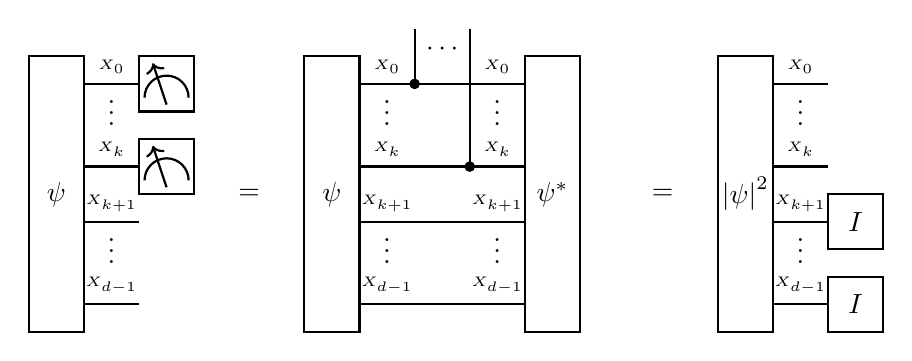
\begin{tikzpicture}[scale=0.35,thick]

    \draw (0,0) rectangle (2,10);
    \node[anchor=center] (text) at (1,5) {$\qstate$};

    \draw (2,1) -- (4,1);

    \draw (2,9) -- (4,9) node[midway,above] {\colorlabelsize $\catvariableof{0}$};
    \drawqcmeasuresymbol{5}{9}
    \node[anchor=center] (text) at (3,8.25) {$\vdots$};
    \draw (2,6) -- (4,6) node[midway,above] {\colorlabelsize $\catvariableof{\atomenumerator}$};
    \drawqcmeasuresymbol{5}{6}

    \draw (2,4) -- (4,4) node[midway,above] {\colorlabelsize $\catvariableof{\atomenumerator+1}$};
    \node[anchor=center] (text) at (3,3.25) {$\vdots$};
    \draw (2,1) -- (4,1) node[midway,above] {\colorlabelsize $\catvariableof{\atomorder-1}$};

    \node[anchor=center] (text) at (8,5) {${=}$};

    \begin{scope}
        [shift={(10,0)}]
        \draw (0,0) rectangle (2,10);
        \node[anchor=center] (text) at (1,5) {$\qstate$};

        \draw (2,1) -- (4,1);

        \draw (2,9) -- (4,9) node[midway,above] {\colorlabelsize $\catvariableof{0}$};
        \node[anchor=center] (text) at (3,8.25) {$\vdots$};
        \draw (2,6) -- (4,6) node[midway,above] {\colorlabelsize $\catvariableof{\atomenumerator}$};

        \drawvariabledot{4}{9}
        \draw (4,9) -- (4,11);

        \drawvariabledot{6}{6}
        \draw (6,6) -- (6,11);

        \node[anchor=center] (text) at (5,10.25) {$\cdots$};

        \draw (4,9) -- (6,9);
        \draw (4,6) -- (6,6);
        \draw (4,4) -- (6,4);
        \draw (4,1) -- (6,1);

        \draw (2,4) -- (4,4) node[midway,above] {\colorlabelsize $\catvariableof{\atomenumerator+1}$};
        \node[anchor=center] (text) at (3,3.25) {$\vdots$};
        \draw (2,1) -- (4,1) node[midway,above] {\colorlabelsize $\catvariableof{\atomorder-1}$};


        \begin{scope}
            [xscale = -1, shift={(-10,0)}]
            \draw (0,0) rectangle (2,10);
            \node[anchor=center] (text) at (1,5) {$\comconqstate$};

            \draw (2,1) -- (4,1);

            \draw (2,9) -- (4,9) node[midway,above] {\colorlabelsize $\catvariableof{0}$};

            \node[anchor=center] (text) at (3,8.25) {$\vdots$};
            \draw (2,6) -- (4,6) node[midway,above] {\colorlabelsize $\catvariableof{\atomenumerator}$};


            \draw (2,4) -- (4,4) node[midway,above] {\colorlabelsize $\catvariableof{\atomenumerator+1}$};
            \node[anchor=center] (text) at (3,3.25) {$\vdots$};
            \draw (2,1) -- (4,1) node[midway,above] {\colorlabelsize $\catvariableof{\atomorder-1}$};
        \end{scope}

    \end{scope}

    \node[anchor=center] (text) at (23,5) {${=}$};

    \begin{scope}
        [shift={(25,0)}]
        \draw (0,0) rectangle (2,10);
        \node[anchor=center] (text) at (1,5) {$\absof{\qstate}^2$};

        \draw (2,1) -- (4,1);

        \draw (2,9) -- (4,9) node[midway,above] {\colorlabelsize $\catvariableof{0}$};
        \node[anchor=center] (text) at (3,8.25) {$\vdots$};
        \draw (2,6) -- (4,6) node[midway,above] {\colorlabelsize $\catvariableof{\atomenumerator}$};

        \draw (2,4) -- (4,4) node[midway,above] {\colorlabelsize $\catvariableof{\atomenumerator+1}$};
        \draw (4,3) rectangle (6,5);
        \node[anchor=center] (text) at (5,4) {$\ones$};
        \node[anchor=center] (text) at (3,3.25) {$\vdots$};
        \draw (2,1) -- (4,1) node[midway,above] {\colorlabelsize $\catvariableof{\atomorder-1}$};
        \draw (4,0) rectangle (6,2);
        \node[anchor=center] (text) at (5,1) {$\ones$};
    \end{scope}

\end{tikzpicture}
    \end{center}
    \caption{Computational Basis Measurement of a quantum state $\qstate$.
    The measurement symbols on the left side indicate the measured qubits and the first equation is understood as a definition.
    In the second equation we sketch, that the measurement distribution is equal to the contraction of the square absolute transform of $\qstate$ to the measured variables.
    }\label{fig:measurementSketch}
\end{figure}

%% Phase-Absolut decomposition
Each complex-valued tensor $\qstatewith$ has a decomposition into a phase tensor $\phasecorewith$ and an absolute tensor $\absof{\qstate}[\shortcatvariables]$ defined by
\begin{align*}
    \qstatewith = \contractionof{\expof{i\cdot\phasecorewith}, \absof{\qstate}[\shortcatvariables]}{\shortcatvariables}\, .
\end{align*}

The measurement distribution is depends only on $\absof{\phi}$, that is
\begin{align*}
    \probwith = \absof{\qstate}^2[\shortcatvariables] \, .
\end{align*}

Note, that when only a subset of variables is measured, the distribution is the contraction of the absolute square transform (these operations do not commute)
\begin{align*}
    \probat{\catvariableof{\variableset}} = \contractionof{\absof{\qstate}^2[\shortcatvariables]}{\catvariableof{\variableset}} \, .
\end{align*}

%% Phasecore vanishing as gauging
When we are interested in the preparation of quantum states with a specific computational basis measurement distribution, we can restrict to states with vanishing phase cores, that is
\begin{align*}
    \qstatewith
    = \contractionof{\expof{i\cdot\zerosat{\shortcatvariables}}, \absof{\qstate}[\shortcatvariables]}{\shortcatvariables}
    = \absof{\qstate}[\shortcatvariables]  \, .
\end{align*}


\subsection{Graph-Controlled circuits}



\begin{definition}[Graph-Controlled Circuit]
    Let $\graph=(\nodes,\edges)$ be a directed acyclic hypergraph, where each hyperedge has exactly one outgoing node and all nodes appear exactly once as outgoing nodes of an hyperedge.
    Then a by $\graph$ controlled circuit is a decoration of the edges $\edge=(\innodes,\{\node\})\in\edges$ by controlled unitaries
    \begin{align*}
        \contunitaryofat{\edge}{\catvariableof{\node,\insymbol},\catvariableof{\node,\outsymbol},\catvariableof{\innodes,\outsymbol}} \, .
    \end{align*}
\end{definition}

\begin{theorem}\label{the:graphControlledPreparesBN}
    Let $\graph$ be a directed acyclic graph.
    The measurement distributions of the by $\graph$ controlled circuits acting on disentangled initial states are equal to the Bayesian Networks on $\graph$.
\end{theorem}

\begin{lemma}
    Any Bayesian network on a directed acyclic graph $\graph$ can be prepared by a $\graph$-controlled circuit with activation circuits of the conditional probability tensors.
\end{lemma}
\begin{proof}
    Let $\probwith$ be a Bayesian network on the graph $\graph$.
    Enumerate the nodes $\nodes$ of the $\graph$ by $[\atomorder]$, such that for each $\catenumeratorin$ we have $\parentsof{\catenumerator}\subset[\catenumerator]$.
    Then define a $\graph$-controlled circuit, by choosing for each $\catenumeratorin$ controlled unitaries which satisfy
    \begin{align*}
        \contunitaryofat{\catenumerator}{\catvariableof{\catenumerator,\insymbol}=0,\catvariableof{\node,\outsymbol},\catvariableof{\parentsof{\catenumerator},\outsymbol}}
        =\sqrt{\condprobof{\catvariableof{\catenumerator}}{\catvariableof{\parentsof{\catenumerator}}}} \, .
    \end{align*}
    Here we specified only the action of the controlled unitary on the basis vector $\onehotmapofat{0}{\catvariableof{\catenumerator}}$, the action on $\onehotmapofat{1}{\catvariableof{\catenumerator}}$ can be chosen by an arbitrary orthogonal unit vector. % Maybe link here the activation circuit scheme, which is already used?
    Any such defined $\graph$-controlled circuit acting on the initial state $\bigotimes_{\catenumeratorin}\onehotmapofat{0}{\catvariableof{\catenumerator}}$ prepares a quantum state $\qstatewith$ with measurement distribution
    \begin{align*}
        \absof{\qstate}^2\left[\shortcatvariables\right] \, .
    \end{align*}
    Given arbitrary $\shortcatindicesin$ we have
        \begin{align*}
        \absof{\qstate}^2\left[\indexedshortcatvariables\right]
            = \prod_{\catenumeratorin} \condprobof{\indexedcatvariableof{\catenumerator}}{\indexedcatvariableof{\parentsof{\catenumerator}}}
            = \probat{\indexedshortcatvariables} \, .
    \end{align*}
    Here we used in the last equation, that $\probwith$ is a Bayesian network.
    Since the equivalence holds for any coordinate, this establishes the equivalence of the measurement distribution of $\qstatewith$ and $\probwith$.
\end{proof}


\begin{lemma}
    Let $(\graph,\contunitary)$ be a $\graph$-controlled circuit acting on a disentangled initial state and $\probat{\nodevariables}$ the corresponding measurement distribution.
    Then we have for each $\node\in\nodes$ the conditional independence
    \begin{align*}
        \condindependent{\catvariableof{\node}}{\catvariableof{\nondescendantsof{\node}}}{\catvariableof{\parentsof{\node}}} \, .
    \end{align*}
\end{lemma}
\begin{proof}
    We choose to a given $\node\in\nodes$ an enumeration $[\catorder]$ of the nodes, such that for each $\catenumeratorin$ we have $\parentsof{\catenumerator}\subset[\catenumerator]$ and for the enumerator $\seccatenumerator$ of $\node$ we further have $\nondescendantsof{\seccatenumerator}\subset[\seccatenumerator]$.
    Let $\probwith$ be the measurement distribution of the $\graph$-controlled circuit acting on a disentangled initial state $\bigotimes_{\catenumeratorin}\qstateofat{\catenumerator}{\catvariableof{\catenumerator}}$ and choose arbitrary $\catindexof{[\catenumerator]}$.
    We then have
    \begin{align*}
        \probat{\catvariableof{\seccatenumerator},\indexedcatvariableof{[\catenumerator]}}
        &= \contractionof{\left(\bigcup_{\catenumeratorin}\{\contunitaryof{\catenumerator},\contunitaryof{\catenumerator,\dagger},\qstateof{\catenumerator},\qstateof{\catenumerator,*}\right)\}
        \cup \left(\bigcup_{\catenumerator\in[\seccatenumerator]} \onehotmapofat{\catindexof{\catenumerator}}{\catvariableof{\catenumerator,\outsymbol}}\right)
        }{
            \catvariableof{\seccatenumerator}
        } \\
        &= \contractionof{\bigcup_{\catenumerator\in[\seccatenumerator]}\{\contunitaryof{\catenumerator},\contunitaryof{\catenumerator,\dagger},\qstateof{\catenumerator},\qstateof{\catenumerator,*},\onehotmapofat{\catindexof{\catenumerator}}{\catvariableof{\catenumerator,\outsymbol}}\}}{
            \catvariableof{\seccatenumerator}
        } \\
        & = \absof{\contractionof{\contunitaryofat{\seccatenumerator}{\catvariableof{\seccatenumerator,\insymbol},\catvariableof{\seccatenumerator,\outsymbol}},\indexedcatvariableof{\parentsof{\seccatenumerator},\outsymbol}}{\catvariableof{\seccatenumerator,\outsymbol}}}^2 \\
        & \quad \quad \cdot \prod_{\catenumerator\in[\seccatenumerator]}
        \left(\contraction{\qstateofat{\catenumerator}{\catvariableof{\catenumerator,\insymbol}},\contunitaryofat{\catenumerator}{\catvariableof{\catenumerator,\insymbol},\catvariableof{\catenumerator,\outsymbol},\indexedcatvariableof{\parentsof{\catenumerator},\outsymbol}}}\right)^2
        %\contraction{\qstateof{\catenumerator,*},\onehotmapofat{\catindexof{\catenumerator}}{\catvariableof{\catenumerator}}}{} \, .
    \end{align*}
    Here we used in the second equation the unitarity of the controlled unitaries to $\catenumerator\notin[\seccatenumerator]$.
    Since the indices $\catindexof{[\seccatenumerator]/\parentsof{\seccatenumerator}} = \catindexof{\nondescendantsof{\seccatenumerator}}$ appear only in the constant term, we conclude
    \begin{align*}
        \condprobat{\catvariableof{\seccatenumerator}}{\catvariableof{[\catenumerator]}} = \condprobat{\catvariableof{\seccatenumerator}}{\catvariableof{\parentsof{\seccatenumerator}}} \otimes \onesat{\catvariableof{\nondescendantsof{\seccatenumerator}}}\, ,
    \end{align*}
    which establishes the conditional independence $\condindependent{\catvariableof{\node}}{\catvariableof{\nondescendantsof{\node}}}{\catvariableof{\parentsof{\node}}}$.
\end{proof}

\begin{proof}[Proof of \theref{the:graphControlledPreparesBN}]
    The theorem follows directly from the two lemmas, using that Bayesian Networks are characterized by the conditional independence of each variable to its non-descendants given its parents.
\end{proof}


Another question is, whether each quantum state, which measurement distribution is a Bayesian Network can be prepared by a $\graph$-controlled circuit.
This is not the case, since the phase tensor of a by $\graph$-controlled circuit has a decomposition
\begin{align*}
    \phasecoreat{\shortcatvariables}
    = \sum_{\catenumeratorin} \phasecoreofat{\catenumerator}{\catvariableof{\catenumerator},\catvariableof{\parentsof{\catenumerator}}} \otimes \onesat{\catvariableof{[\catorder]/\{\{\catenumerator\}\cup\parentsof{\catenumerator}\}}} \, ,
\end{align*}
where the phase cores $\phasecoreof{\catenumerator}$ can be read of the controlled unitaries.
    \section{Circuit Encoding Schemes}

We investigate here quantum pendants to the function encoding schemes used in \tnreason{}{}.

\begin{itemize}
    \item Pendant for Coordinate Encoding in \tnreason{}: Amplitude Encoding, storing the function value in the amplitude of an ancilla qubit.
    This is realized by an \textbf{\ActivationCircuit{}}.
    \item Pendant for Basis Encoding in \tnreason{}: \textbf{\ComputationCircuit{}}, with composition by contraction property.
\end{itemize}

Both are defined using controlled single qubit gates (see Sections 4.2-3 in [Nielsen, Chuang]) with ancilla qubits being the target qubits. % where the incoming qubit variable is $\avariableof{\insymbol}$ and the outgoing $\avariableof{\outsymbol}$.

\subsection{\ActivationCircuit{}}


%% Angle preparing
We define the angle preparing function on $p\in[0,1]$ by
\begin{align*}
    h(p) = 2 \cdot \mathrm{cos}^{-1}\left(\sqrt{1-p}\right) \, .
\end{align*}
For any $p\in[0,1]$ we then have
\begin{align*}
    \contractionof{\onehotmapofat{0}{\avariableof{\insymbol}},\yrotationofat{h(p)}{\avariableof{\insymbol},\avariableof{\outsymbol}}}{\avariableof{\outsymbol}}
    = \begin{bmatrix}
          \sqrt{1-p} \\
          \sqrt{p}
    \end{bmatrix} \, .
\end{align*}

\begin{definition}[\ActivationCircuit{}]
    Given a function
    \begin{align*}
        \exfunction : \bigtimes_{\selindexin} [2] \rightarrow [0,1]
    \end{align*}
    its \activationCircuit{} is the controlled unitary
    $\qcaencodingofat{\hypercore}{\avariableof{\insymbol},\avariableof{\outsymbol},\headvariableof{[\seldim]}}$ defined as
    \begin{align*}
        \qcaencodingofat{\hypercore}{\avariableof{\insymbol},\avariableof{\outsymbol},\headvariableof{[\seldim]}}
        = \sum_{\headindexof{[\seldim]}} \onehotmapofat{\headindexof{[\seldim]}}{\headvariableof{[\seldim]}}
        %\otimes \onehotmapofat{\headindexof{[\seldim]}}{\headvariableof{\insymbol,[\seldim]}}
        \otimes \yrotationofat{h(\exfunctionat{\headindexof{[\seldim]}})}{\avariableof{\insymbol},\avariableof{\outsymbol}} \, .
    \end{align*}
\end{definition}

%% Drop the in and out
We will ease our notation by dropping the $\insymbol$ and $\outsymbol$ labels to the control variables.
This amounts to understanding the Dirac delta tensors in \activationCircuits{} as hyperedges.
Along that picture the quantum circuit is a tensor network on hyperedges instead of edges.


When we have a probability tensor, its \activationCircuit{} be prepared, since all values are in $[0,1]$.
Note that for rejection sampling, only the quotients of the values are important, we can therefore scale the value by a scalar such that the mode is $1$.

Tensors $\hypercoreat{\headvariables}$ with non-negative coordinates can be encoded after dividing them by their maximum, that is the \activationCircuit{} of the function
\begin{align*}
    \exfunctionat{\headindexof{[\seldim]}} = \frac{\hypercoreat{\headvariables=\headindexof{[\seldim]}}}{\max_{\secheadindexof{[\seldim]}} \hypercoreat{\headvariables=\secheadindexof{[\seldim]}}}
\end{align*}
When the maximum of the tensor is not known, it can be replaced by an upper bound (reducing the acceptance rate of the rejection sampling).

\subsubsection{Encoding of directed tensors}

Following the schemes in \cite{low_quantum_2014}, we can prepare the acyclic networks of directed and non-negative tensors by a sequence of controlled rotations.
Directed and non-negative tensors correspond with conditional probability distributions and acyclic networks are Bayesian Networks.
We prepare them by \activationCircuit{}s of functions (see \figref{fig:cpdEncoding})
\begin{align*}
    \catindexof{\parentsof{\catenumerator}} \rightarrow \condprobat{\catvariableof{\catenumerator}=1}{\indexedcatvariableof{\parentsof{\catenumerator}}} \, .
\end{align*}

In this way, Bayesian Networks can be prepared as quantum circuits, where each conditional probability distribution is prepared by an \activationCircuit{}.

\begin{theorem}[Low et al.]
    Any Bayesian Network of variables $\shortcatvariables$, where the enumeration by $[\atomorder]$ respects the partial order by child-parent relations, can be prepared as a quantum circuit by concatenating the \activationCircuit{}s
    \begin{align*}
        \qcaencodingofat{
            \condprobat{\catvariableof{\catenumerator}=1}{\catvariableof{\parentsof{\catenumerator}}}
        }{\catvariableof{\catenumerator,\insymbol},\catvariableof{\catenumerator},\catvariableof{\parentsof{\catenumerator}},\catvariableof{\parentsof{\catenumerator}}}
    \end{align*}
    for $\atomenumeratorin$ and acting on the initial state $\bigotimes_{\atomenumeratorin}\onehotmapofat{0}{\catvariableof{\catenumerator,\insymbol}}$ .
\end{theorem}


%To this end, one iterates over the states of the incoming variables, and performs a controlled rotation on the outgoing variable, where the angle is given by the value of the tensor at the incoming state.
%This generalizes the basis encoding scheme, which demands boolean tensors.

\begin{figure}
    \begin{center}
        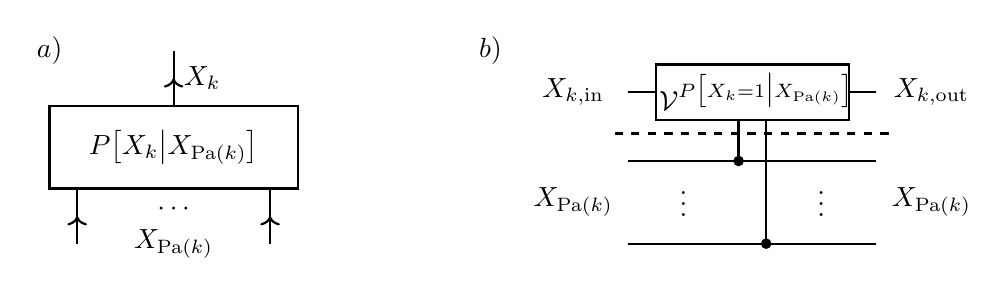
\begin{tikzpicture}[scale=0.35,thick] % , baseline = -3.5pt

    \node[anchor=center] (text) at (16,1) {${b)}$};

    \begin{scope}
        [shift={(20,-7)}]

        \node[anchor=center] (text) at (-1,6.5) {$\catvariableof{\catenumerator,\insymbol}$};
        \node[anchor=center] (text) at (12,6.5) {$\catvariableof{\catenumerator,\outsymbol}$};

        \draw (5,4) -- (5,5.5);
        \drawvariabledot{5}{4}
        \draw (6,1) -- (6,5.5);
        \drawvariabledot{6}{1}

        \draw (1,6.5) -- (2,6.5);
        \draw (2,5.5) rectangle (9,7.5);
        \node[anchor=center] (text) at (5.65,6.5) {$\qcaencodingof{\condprobof{\catvariableof{\catenumerator}=1}{\catvariableof{\parentsof{\catenumerator}}} }$};
        \draw (9,6.5) -- (10,6.5);

        \draw[dashed] (0.5,5) -- (10.5,5);

        \draw (1,4) -- (10,4);

        \node[anchor=center] (text) at (3,2.75) {$\vdots$};
        \node[anchor=center] (text) at (-1,2.5) {$\catvariableof{\parentsof{\catenumerator}}$};

        \node[anchor=center] (text) at (8,2.75) {$\vdots$};
        \node[anchor=center] (text) at (12,2.5) {$\catvariableof{\parentsof{\catenumerator}}$};

        \draw (1,1) -- (10,1);

    \end{scope}


    \node[anchor=center] (text) at (0,1) {${a)}$};

    \draw[->-] (4.5,-1) -- (4.5,1) node[midway, right]{$\catvariableof{\catenumerator}$};
    \draw (0,-1) rectangle (9,-4);
    \node[anchor=center] (text) at (4.5,-2.5) { $\condprobof{\catvariableof{\catenumerator}}{\catvariableof{\parentsof{\catenumerator}}} $};
    \draw[->-] (1,-6) -- (1,-4);

    \node[anchor=center] (text) at (4.5,-4.75) {$\cdots$};
    \node[anchor=center] (text) at (4.5,-6) {$\catvariableof{\parentsof{\catenumerator}}$};

    \draw[->-] (8,-6) -- (8,-4);


\end{tikzpicture}
    \end{center}
    \caption{
        Representation of directed and positive tensor by a controlled rotation.
        a) Conditional probability tensor $\condprobat{\catvariableof{\catenumerator}}{\catvariableof{\parentsof{\catenumerator}}}$ being a tensor in a Bayesian Network.
        b) Circuit Encoding as a controlled rotation, which is the \ActivationCircuit{} of the tensor $\condprobat{\catvariableof{\catenumerator}=1}{\catvariableof{\parentsof{\catenumerator}}}$.
    }\label{fig:cpdEncoding}
\end{figure}

\subsection{\ComputationCircuits{}}

We here suggest a quantum pendant to basis encodings (see Chapter Basis Calculus), which has the decomposition by contraction property.

\begin{definition}[\ComputationCircuit{}]
    Given a boolean function $\exfunction:\atomstates\rightarrow[2]$ the \computationCircuit{} is the unitary tensor
    \begin{align*}
        \qcbencodingofat{\exfunction}{\headvariableof{\insymbol,\exfunction},\headvariableof{\outsymbol,\exfunction},\shortcatvariables}
        &\quad=
        \sum_{\shortcatindicesin\wcols\exfunctionat{\shortcatindices}=1}
        \paulixat{\headvariableof{\insymbol,\exfunction},\headvariableof{\outsymbol,\exfunction}} \otimes
        \onehotmapofat{\shortcatindices}{\shortcatvariables} \\ % \otimes \onehotmapofat{\shortcatindices}{\catvariableof{\outsymbol,[\atomorder]}} \\
        & \quad \quad \quad +
        \sum_{\shortcatindicesin\wcols\exfunctionat{\shortcatindices}=0}
        \identityat{\headvariableof{\insymbol,\exfunction},\headvariableof{\outsymbol,\exfunction}} \otimes
        \onehotmapofat{\shortcatindices}{\shortcatvariables} \, . % \otimes \onehotmapofat{\shortcatindices}{\catvariableof{\outsymbol,[\atomorder]}}
    \end{align*}
\end{definition}

Notice, that $U^{\lnot} = \mathrm{CNOT}$, which is obvious from $\onesat{\headvariableof{\insymbol},\headvariableof{\outsymbol}} - \identityat{\headvariableof{\insymbol},\headvariableof{\outsymbol}}$ being the Pauli-X gate (not to be confused with $X$ denoting distributed variables here).
The \computationCircuit{} is therefore a generalized controlled $\mathrm{NOT}$ gate, where the control is by a boolean function.

Functions with multiple output variables, i.e. $\exfunction:\atomstates\rightarrow\bigtimes_{\selindexin}[2]$, can be encoded image coordinate wise as a concatenation of the respective circuits.

\subsubsection{Composition by Contraction - Exploiting \DecompositionSparsity{}}

The decomposition by contraction property of basis encodings is now a composition of circuits property, as stated in the next lemma.

\begin{lemma}
    We have for functions $\exfunction:\atomstates\rightarrow\bigtimes_{\selindexin}[2]$, $\secexfunction:\bigtimes_{\selindexin}[2]\rightarrow\bigtimes_{s\in[r]}[2]$ (see \figref{fig:qcbencodingDecomposition})
    \begin{align*}
        \qcbencodingofat{\secexfunction\circ\exfunction}{\headvariableof{\insymbol,\secexfunction\circ\exfunction},\headvariableof{\outsymbol,\secexfunction\circ\exfunction},\catvariableof{\insymbol,[\atomorder]},\catvariableof{\outsymbol,[\atomorder]}}
        = \breakablecontractionof{
            &\onehotmapofat{0}{\headvariableof{\insymbol,\exfunction}},\\
            &\qcbencodingofat{\exfunction}{\headvariableof{\insymbol,\exfunction},\headvariableof{\outsymbol,\exfunction},\catvariableof{\insymbol,[\atomorder]},\catvariableof{\outsymbol,[\atomorder]}},\\
            &\qcbencodingofat{\secexfunction}{\headvariableof{\insymbol,\secexfunction\circ\exfunction},\headvariableof{\outsymbol,\secexfunction\circ\exfunction},\headvariableof{\outsymbol,\exfunction},\headvariableof{\outsymbol,\exfunction}}
        }{
            \headvariableof{\insymbol,\secexfunction\circ\exfunction},\headvariableof{\outsymbol,\secexfunction\circ\exfunction},\catvariableof{\insymbol,[\atomorder]},\catvariableof{\outsymbol,[\atomorder]}
        } \, .
    \end{align*}
\end{lemma}

When having a syntactical decomposition of a propositional formula, we can iteratively apply the \computationCircuit{} decomposition theorem and prepare each connective by a circuit.
We can decompose any propositional formula into logical connectives and prepare to each a modulus 2 circuit implementation.
This works, when the target qubit of one connective is used as a value qubit of another.

\begin{figure}
    \begin{center}
        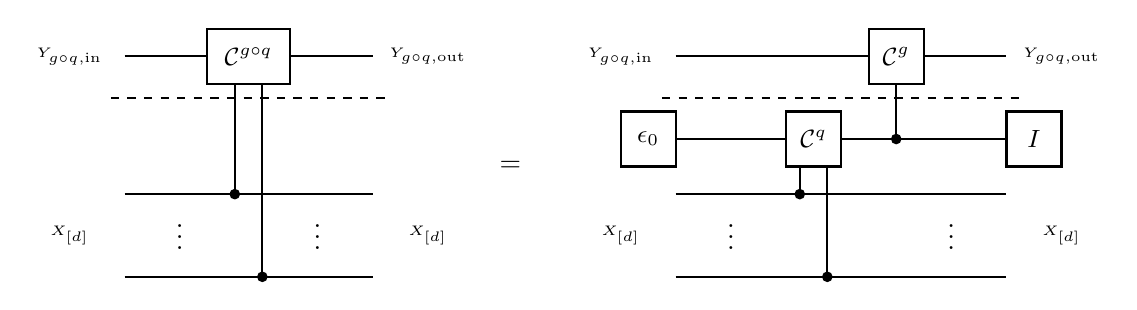
\begin{tikzpicture}[scale=0.35, thick] % , baseline = -3.5pt

    %% Statistic Qubits
    \node[anchor=center] (text) at (-1,9) {\colorlabelsize $\headvariableof{\secexfunction\circ\exfunction,\insymbol}$};
    \node[anchor=center] (text) at (15,9) {\colorlabelsize $\headvariableof{\secexfunction\circ\exfunction,\outsymbol}$};

    \draw (1,9) -- (8,9);
    \draw (8,8) rectangle (10,10);
    \node[anchor=center] (text) at (9,9) {\corelabelsize $\qcbencodingof{\secexfunction}$};
    \draw (10,9) -- (13,9);

    \draw (9,6) -- (9,8);
    \drawvariabledot{9}{6}

    \draw (-1,5) rectangle (1,7);
    \node[anchor=center] (text) at (0,6) {\corelabelsize $\onehotmapof{0}$};
    \draw (1,6) -- (5,6);
    \draw (5,5) rectangle (7,7);
    \node[anchor=center] (text) at (6,6) {\corelabelsize $\qcbencodingof{\exfunction}$};
    \draw (7,6) -- (13,6);
    \draw (13,5) rectangle (15,7);
    \node[anchor=center] (text) at (14,6) {\corelabelsize $\ones$};


    \draw (5.5,4) -- (5.5,5);
    \drawvariabledot{5.5}{4}
    \draw (6.5,1) -- (6.5,5);
    \drawvariabledot{6.5}{1}

    \draw[dashed] (0.5,7.5) -- (13.5,7.5);

    \draw (1,4) -- (13,4);

    \node[anchor=center] (text) at (3,2.75) {$\vdots$};
    \node[anchor=center] (text) at (-1,2.5) {\colorlabelsize $\shortcatvariables$};

    \node[anchor=center] (text) at (11,2.75) {$\vdots$};
    \node[anchor=center] (text) at (15,2.5) {\colorlabelsize $\shortcatvariables$};

    \draw (1,1) -- (13,1);

    \node[anchor=center] (text) at (-5,5) {${=}$};

    \begin{scope}
        [shift={(-20,0)}]

        \node[anchor=center] (text) at (-1,9) {\colorlabelsize $\headvariableof{\secexfunction\circ\exfunction,\insymbol}$};
        \node[anchor=center] (text) at (12,9) {\colorlabelsize $\headvariableof{\secexfunction\circ\exfunction,\outsymbol}$};

        \draw (5,4) -- (5,8);
        \drawvariabledot{5}{4}
        \draw (6,1) -- (6,8);
        \drawvariabledot{6}{1}

        \draw (1,9) -- (4,9);
        \draw (4,8) rectangle (7,10);
        \node[anchor=center] (text) at (5.5,9) {\corelabelsize $\qcbencodingof{\secexfunction\circ\exfunction}$};
        \draw (7,9) -- (10,9);

        \draw (1,4) -- (10,4);

        \draw[dashed] (0.5,7.5) -- (10.5,7.5);

        \node[anchor=center] (text) at (3,2.75) {$\vdots$};
        \node[anchor=center] (text) at (-1,2.5) {\colorlabelsize $\shortcatvariables$};

        \node[anchor=center] (text) at (8,2.75) {$\vdots$};
        \node[anchor=center] (text) at (12,2.5) {\colorlabelsize $\shortcatvariables$};

        \draw (1,1) -- (10,1);

    \end{scope}

\end{tikzpicture}
    \end{center}
    \caption{
        Exploitaition of \DecompositionSparsity{} in \computationCircuit{}s.
    }\label{fig:qcbencodingDecomposition}
\end{figure}


%    \begin{lemma}
%        We have for functions $\exfunction:\atomstates\rightarrow\bigtimes_{\selindexin}[2]$, $\secexfunction:\bigtimes_{\selindexin}[2]\rightarrow\bigtimes_{s\in[r]}[2]$
%        \begin{align*}
%            \qcbencodingofat{\secexfunction\circ\exfunction}{\catvariableof{\insymbol,[\atomorder]},\catvariableof{\outsymbol,[\atomorder]},\headvariableof{\insymbol,\secexfunction\circ\exfunction},\headvariableof{\outsymbol,\secexfunction\circ\exfunction}}
%            = \breakablecontractionof{
%                &\onehotmapofat{0}{\headvariableof{\insymbol,\exfunction}},\\
%                &\qcbencodingofat{\exfunction}{\catvariableof{\insymbol,[\atomorder]},\catvariableof{\outsymbol,[\atomorder]},\headvariableof{\insymbol,\exfunction},\headvariableof{\outsymbol,\exfunction}},\\
%                &\qcbencodingofat{\secexfunction}{\headvariableof{\outsymbol,\exfunction},\headvariableof{\outsymbol,\mathrm{aux}},\headvariableof{\insymbol,\secexfunction\circ\exfunction},\headvariableof{\outsymbol,\secexfunction\circ\exfunction}}
%            }{
%                \catvariableof{\insymbol,[\atomorder]},\catvariableof{\outsymbol,[\atomorder]},\headvariableof{\insymbol,\secexfunction\circ\exfunction},\headvariableof{\outsymbol,\secexfunction\circ\exfunction}
%            } \, .
%        \end{align*}
%    \end{lemma}

Note, that the variables $\headvariableof{\outsymbol,\mathrm{aux}}$ are auxiliar and not left open in the contraction.
This amounts to not measuring them in a computational basis measurement.

\subsubsection{Construction for mod2-basis+ CP decompositions - Exploiting \PolynomialSparsity{}}

Concatenating two \computationCircuit{}s, which have the same head qubit, is the \computationCircuit{} of their mod2 sum.

A basis+ elementary function can be encoded by a single controlled NOT operation with auxiliary X qubits.

This motivates the mod2-basis+ CP decomposition of tensors, which is exactly the decomposition of boolean polynomials into monomials.
Each monomial is called a terms (products of x or (1-x) factors), and minterms in case that all variables appear.

\begin{definition}
    Given a boolean tensor $\hypercore$, a mod2-basis+ CP decomposition is a collection $\sliceset$ of tuples $(\variableset,\catindexof{\variableset})$ with such that for any $\shortcatindicesin$
    \begin{align*}
        \hypercoreat{\indexedshortcatvariables}
        = \bigoplus_{(\variableset,\catindexof{\variableset})\in\sliceset} \contractionof{\onehotmapofat{\catindexof{\variableset}}{\catvariableof{\variableset}}}{\indexedshortcatvariables} \, .
    \end{align*}
\end{definition}

Using that basis CP decompositions are a special case of basis+ CP decompositions, we get the following rank bound.

\begin{lemma}
    The mod2-basis+ CP rank is bounded by the basis CP rank.
\end{lemma}
\begin{proof}
    Use $\variableset=[\atomorder]$, and $\catindexof{\variableset}$ to each supported state.
    Then the mod2-sum is a usual sum and the basis CP decomposition is also a mod2-basis+ CP decomposition.
\end{proof}

This shows in particular, that any propositional formula can be represented by a mod2-basis+ CP decomposition.

\begin{lemma}
    The \computationCircuit{} to a boolean tensor $\hypercore$ with a mod2-basis+ CP decomposition $\sliceset$ obeys
    \begin{align*}
        &\qcbencodingofat{\hypercore}{
            \headvariableof{\hypercore,\insymbol},\headvariableof{\hypercore,\outsymbol},\catvariableof{[\atomorder],\insymbol},\catvariableof{[\atomorder],\insymbol}
        } \\
        & \quad =
        \breakablecontractionof{
            \{\identityat{\headvariableof{\hypercore,\insymbol},\headvariableof{0}},\identityat{\headvariableof{\hypercore,\outsymbol},\headvariableof{\cardof{\sliceset}-1}}\} \cup
            \{\qcbencodingofat{\onehotmapof{\catindexof{\variableset}}}{
                \headvariableof{\decindex}, \headvariableof{\decindex+1},
                \catvariableof{\variableset,\insymbol},\catvariableof{\variableset,\outsymbol}} \wcols (\variableset,\catindexof{\variableset})\in\sliceset\}
        }{\headvariableof{\hypercore,\insymbol},\headvariableof{\hypercore,\outsymbol},\catvariableof{[\atomorder],\insymbol},\catvariableof{[\atomorder],\outsymbol}}
    \end{align*}
    where $\decindex\in[\cardof{\sliceset}]$ enumerates the tuples in $\sliceset$.
\end{lemma}

Each \computationCircuit{} to each boolean monomial can be prepared by a multiple-controlled $\paulixsymbol$ gate and further pairs of $\paulixsymbol$ gates preparing the control state, see \figref{fig:qcbencodingPolynomial}. %where the control qubits are the affected variables and the target qubit is the value qubit.
When we sum monomials wrt modulus 2 calculus, then the preparation is a sequence of such circuits.
In such way, we can prepare the \computationCircuit{} to any propositional formula.
This encoding strategy exploits a modified (by mod2 calculus) \polynomialSparsity{}.

\begin{figure}
    \begin{center}
        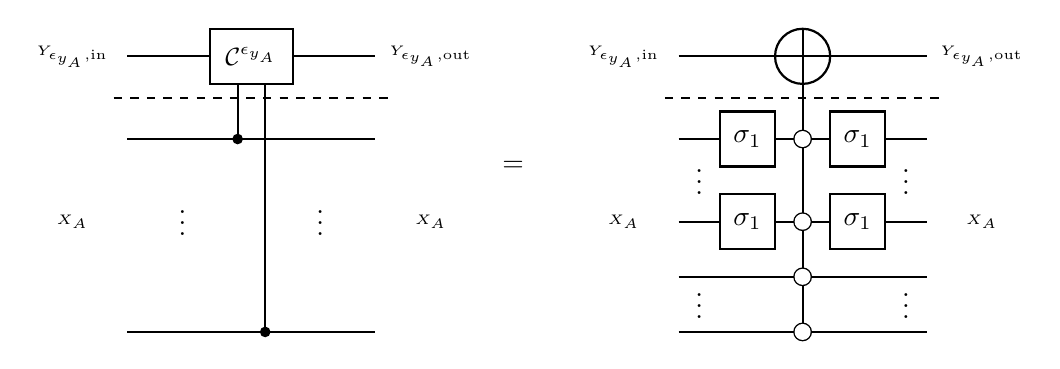
\begin{tikzpicture}[scale=0.35, thick] % , baseline = -3.5pt

    \node[anchor=center] (text) at (-5,4) {${=}$};

    \begin{scope}
        [shift={(-20,-1)}]

        \node[anchor=center] (text) at (-1,9) {\colorlabelsize $\headvariableof{\onehotmapof{\headindexof{\variableset}},\insymbol}$};
        \node[anchor=center] (text) at (12,9) {\colorlabelsize $\headvariableof{\onehotmapof{\headindexof{\variableset}},\outsymbol}$};

        \draw (5,6) -- (5,8);
        \drawvariabledot{5}{6}
        \draw (6,-1) -- (6,8);
        \drawvariabledot{6}{-1}

        \draw (1,9) -- (4,9);
        \draw (4,8) rectangle (7,10);
        \node[anchor=center] (text) at (5.5,9) {\corelabelsize $\qcbencodingof{\onehotmapof{\headindexof{\variableset}}}$};
        \draw (7,9) -- (10,9);

        \draw (1,6) -- (10,6);

        \draw[dashed] (0.5,7.5) -- (10.5,7.5);

        \node[anchor=center] (text) at (3,3.25) {$\vdots$};
        \node[anchor=center] (text) at (-1,3) {\colorlabelsize $\catvariableof{\variableset}$};

        \node[anchor=center] (text) at (8,3.25) {$\vdots$};
        \node[anchor=center] (text) at (12,3) {\colorlabelsize $\catvariableof{\variableset}$};

        \draw (1,-1) -- (10,-1);

    \end{scope}

    \node[anchor=center] (text) at (-1,8) {\colorlabelsize $\headvariableof{\onehotmapof{\headindexof{\variableset}},\insymbol}$};
    \node[anchor=center] (text) at (12,8) {\colorlabelsize $\headvariableof{\onehotmapof{\headindexof{\variableset}},\outsymbol}$};

    %% CNOT
    \draw (1,8) -- (10,8);
    \draw (5.5,8) circle (1);

    \draw[dashed] (0.5,6.5) -- (10.5,6.5);

    \draw (1,5) -- (2.5,5);
    \draw (2.5,4) rectangle (4.5,6);
    \node[anchor=center] (text) at (3.5,5) {$\paulixsymbol$};
    \draw (4.5,5) -- (6.5,5);
    \draw (6.5,4) rectangle (8.5,6);
    \node[anchor=center] (text) at (7.5,5) {$\paulixsymbol$};
    \draw (8.5,5) -- (10,5);

    \node[anchor=center] (text) at (1.75,3.75) {$\vdots$};
    \node[anchor=center] (text) at (9.25,3.75) {$\vdots$};

    \draw (1,2) -- (2.5,2);
    \draw (2.5,1) rectangle (4.5,3);
    \node[anchor=center] (text) at (3.5,2) {$\paulixsymbol$};
    \draw (4.5,2) -- (6.5,2);
    \draw (6.5,1) rectangle (8.5,3);
    \node[anchor=center] (text) at (7.5,2) {$\paulixsymbol$};
    \draw (8.5,2) -- (10,2);

    \draw (1,0) -- (10,0);
    \draw (1,-2) -- (10,-2);

    \node[anchor=center] (text) at (1.75,-0.75) {$\vdots$};
    \node[anchor=center] (text) at (9.25,-0.75) {$\vdots$};

    \node[anchor=center] (text) at (-1,2) {\colorlabelsize $\catvariableof{\variableset}$};
    \node[anchor=center] (text) at (12,2) {\colorlabelsize $\catvariableof{\variableset}$};

    \draw (5.5,-2) -- (5.5,9);
    \drawcontroldot{5.5}{5}
    \drawcontroldot{5.5}{2}
    \drawcontroldot{5.5}{0}
    \drawcontroldot{5.5}{-2}


\end{tikzpicture}
    \end{center}
    \caption{
        Exploitaition of \PolynomialSparsity{} in \computationCircuit{}s.
        Here, we use the typical denotation of a muliple-controlled CNOT gate, which control symbols do not indicate Dirac tensors.
    }\label{fig:qcbencodingPolynomial}
\end{figure}

\subsubsection{Preparation by fine and coarse structure}

Having a mod2-basis+ CP decomposition of rank $r$ to a connective, we need $r$ controlled NOT gates to prepare the basis encoding.
Given a syntactical decomposition of a boolean statistics, we prepare the basis encoding as a circuit with:
\begin{itemize}
    \item \textbf{Fine Structure:} Represent each logical connective based on its mod2-basis+ CP decomposition, as a concatenation of \computationCircuit{}s with the same variables.
    \item \textbf{Coarse Structure:} Arrange the logical connective representing circuits according to the syntactical hypergraph, where parent head variables appear as distributed variables at their children.
\end{itemize}
    \section{Sampling from \ComputationActivationNetworks{}}

We investigate, how the above circuit encoding schemes can be applied in the preparation of states, which computational basis measurements are samples from specific distributions.

In particular, we build graph-controlled circuits being compositions of \computationCircuits{} and \activationCircuits{}, for which specific conditional distributions coincide with \ComputationActivationNetworks{}.

\subsection{Preparing ancilla augmented distributions for \ComputationActivationNetworks{}}

The computation network consists already of directed cores and therefore is already a Bayesian network.
The activation network however needs ancilla augmentation.
Therefore we have:
\begin{itemize}
    \item Pendant for Coordinate Encoding in \tnreason{}: Amplitude Encoding, storing the function value in the amplitude of an ancilla qubit.
    This is realized by an \textbf{\ActivationCircuit{}} acting on an ancilla qubit in the ground state.
    \item Pendant for Basis Encoding in \tnreason{}: \textbf{\ComputationCircuit{}}, with composition by contraction property.
    Applied on the ground state, the \computationCircuit{} generates the basis encoding quantum state, which is parallel to the basis encoding.
\end{itemize}
Both are defined using controlled single qubit gates (see Sections 4.2-3 in \cite{nielsen_quantum_2010}) with ancilla qubits being the target qubits. % where the incoming qubit variable is $\avariableof{\insymbol}$ and the outgoing $\avariableof{\outsymbol}$.


For elementary \ComputationActivationNetworks{}, we can prepare ancilla variables having single parents, corresponding with the ancilla augmentation of an elementary tensor.
For an example, see \figref{fig:toyAccounting}.

To a generic activation hypergraph $\graph$, we would do ancilla augmentation for the activation tensor network, where each hidden variable is prepared by an additional qubit in uniform state (i.e. a Hadamard gate acting on a ground state).

\subsection{Amplitude Amplification}

Literature:
\begin{itemize}
    \item \cite{grover_fast_1996} Grover algorithm (search in unstructured database)
    \item \cite{ozols_quantum_2013} introduced quantum rejection sampling (using amplitude amplification)
    \item \cite{low_quantum_2014} used quantum rejection sampling for Bayesian network sampling (which is NP-hard when conditioned on evidence, see e.g. \cite{koller_probabilistic_2009})
\end{itemize}

Note, that the variable qubits are uniformly distributed when only the computation circuit is applied.
When sampling the probability distribution, we need the ancilla qubits to be in state $1$ in order for the sample to be valid.
Any other states will have to be rejected.

Classically, this can be simulated in the same way:
Just draw the variables from uniform, calculate the value qubit by a logical circuit inference and accept with probability by the computed value.

For this procedure to be more effective (and in particular not having an efficient classical pendant), we need amplitude amplification on the value qubit.
This can provide a square root speedup in the complexity compared with classical rejection sampling.

\textbf{Open Question:} Is there a way to avoid amplitude amplification and use a more direct circuit implementation of the activation network?
- Cannot be the case, when the encoding is determined by the activation tensor alone: Needs to use the computated statistic as well.

\subsection{Sampling from \ComputationActivationNetworks{} as Quantum Circuits}

\red{So far: Sample from \HybridLogicNetworks{}, would need qudits for more general \ComputationActivationNetworks{}.
Can do non-elementary \ComputationActivationNetworks{}, when activating whole activation core.}

\tnreason{} provides tensor network representations of knowledge bases and exponential families following a Computation Activation architecture.
Here are some ideas to utilize quantum circuits for sampling from \ComputationActivationNetworks{}.
We can produce Q-samples for ancilla augmented \ComputationActivationNetworks{}  using \computationCircuits{} and \activationCircuits{}:
\begin{itemize}
    \item For each (sub-) statistic, prepare a qubit by \ComputationCircuits{}
    \item Based on the computed qubits, prepare ancilla qubits by \ActivationCircuits{} to the activation cores.
\end{itemize}

\begin{figure}
    \begin{center}
        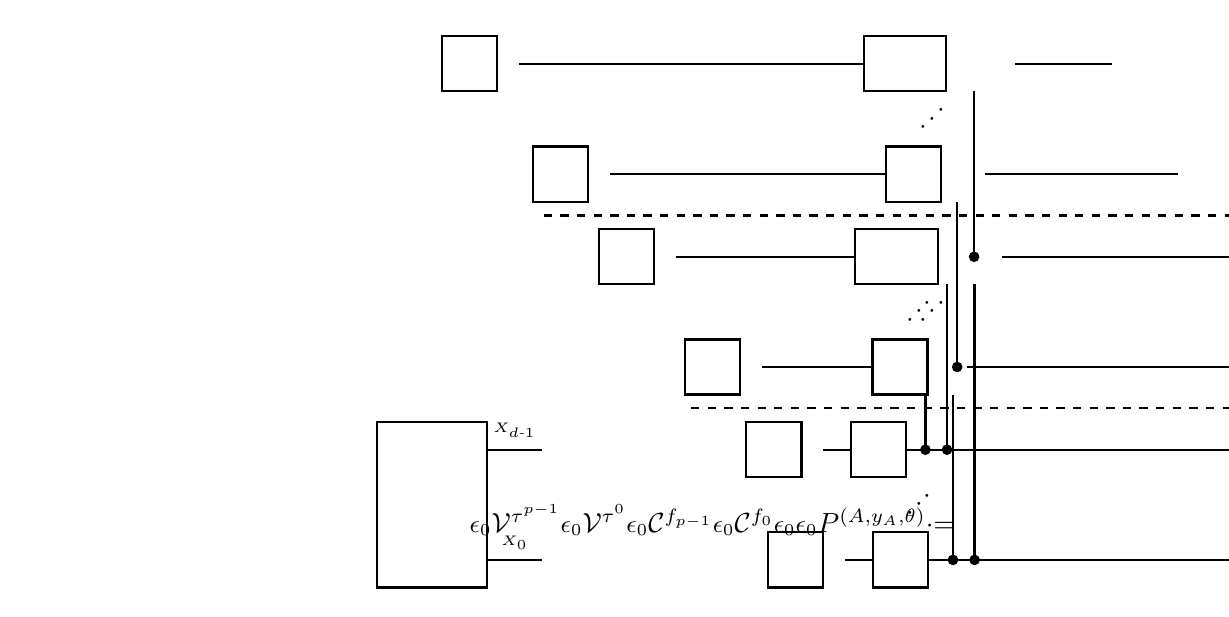
\begin{tikzpicture}[scale=0.35, thick]
    %% Ancilla Qubits
    \draw (-1,16) rectangle (1,18);
    \drawtextnode{0}{17}{\corelabelsize $\fbasis$}
    \draw (1,17) -- (13.5,17);
    \draw (13.5,16) rectangle (16.5,18);
    \drawtextnode{15}{17}{$\qcaencodingof{\hypercoreof{\seldim-1}}$};
    \draw (16.5,17) -- (20,17);

    \draw (15,10) -- (15,16);
    \drawvariabledot{15}{10}

    \node[rotate=45] at (13.5,15) {$\cdots$};
    \node[rotate=45] at (13.5,8) {$\cdots$};

    \drawtextnode{0}{15.25}{$\vdots$};
    \drawtextnode{-3.5}{15}{Ancilla\\Qubits};

    \draw (-1,12) rectangle (1,14);
    \drawtextnode{0}{13}{\corelabelsize $\fbasis$};
    \draw (1,13) -- (11,13);
    \draw (11,12) rectangle (13,14);
    \drawtextnode{12}{13}{$\qcaencodingof{\hypercoreof{0}}$};
    \draw (13,13) -- (20,13);

    \draw (12,6) -- (12,12);
    \drawvariabledot{12}{6}

    %% Statistic Qubits
    \draw[dashed] (-3,11.5) -- (26.5,11.5);
    \draw (-1,9) rectangle (1,11);
    \drawtextnode{0}{10}{\corelabelsize $\fbasis$};
    \draw (1,10) -- (7.5,10);
    \draw (7.5,9) rectangle (10.5,11);
    \drawtextnode{9}{10}{$\qcbencodingof{f_{\seldim-1}}$};
    \draw (10.5,10) -- (20,10);

    \draw (8.5,3) -- (8.5,9);
    \drawvariabledot{8.5}{3}
    \draw (9.5,-1) -- (9.5,9);
    \drawvariabledot{9.5}{-1}

    \node[rotate=45] at (7.5,8) {$\cdots$};
    \node[rotate=45] at (7.5,1) {$\cdots$};

    \drawtextnode{0}{8.25}{$\vdots$};
    \drawtextnode{-3.5}{8}{Statistic\\Qubits};

    \draw (-1,5) rectangle (1,7);
    \drawtextnode{0}{6}{\corelabelsize $\fbasis$};
    \draw (1,6) -- (5,6);
    \draw (5,5) rectangle (7,7);
    \drawtextnode{6}{6}{$\qcbencodingof{f_{0}}$};
    \draw (7,6) -- (20,6);

    \draw (5.5,3) -- (5.5,5);
    \drawvariabledot{5.5}{3}
    \draw (6.5,-1) -- (6.5,5);
    \drawvariabledot{6.5}{-1}

    %% Distributed Qubits
    \draw[dashed] (-3,4.5) -- (26.5,4.5);

    \draw (-1,2) rectangle (1,4);
    \drawtextnode{0}{3}{\corelabelsize $\fbasis$};
    \draw (1,3) -- (2,3);
    \draw (2,2) rectangle (4,4);
    \drawtextnode{3}{3}{\corelabelsize $\hgate$};

    \draw (4,3) -- (20,3);

    \drawtextnode{0}{1.25}{$\vdots$};
    \drawtextnode{-3.5}{1}{Distributed\\Qubits};

    \draw (-1,-2) rectangle (1,0);
    \drawtextnode{0}{-1}{\corelabelsize $\fbasis$};
    \draw (1,-1) -- (2,-1);
    \draw (2,-2) rectangle (4,0);
    \drawtextnode{3}{-1}{\corelabelsize $\hgate$};

    \draw (4,-1) -- (20,-1);

    %% Measurements
    \drawqcmeasuresymbol{21}{17}
    \draw (22,17) -- (24,17) node[midway,above]{\colorlabelsize $\avariableof{\seldim\shortminus1}$};
    \draw (24,16) rectangle (26,18);
    \node[anchor=center] at (25,17) {\corelabelsize $\tbasis$};

    \drawtextnode{23}{15.5}{$\vdots$};
    \drawqcmeasuresymbol{21}{13}
    \draw (22,13) -- (24,13) node[midway,above]{\colorlabelsize $\avariableof{0}$};
    \draw (24,12) rectangle (26,14);
    \node[anchor=center] at (25,13) {\corelabelsize $\tbasis$};

    \drawqcmeasuresymbol{21}{10}
    \draw (22,10) -- (24,10) node[midway,above]{\colorlabelsize $\headvariableof{\seldim\shortminus1}$};
    \drawvariabledot{24}{10}
    \drawtextnode{23}{8.5}{$\vdots$};
    \drawqcmeasuresymbol{21}{6}
    \draw (22,6) -- (24,6) node[midway,above]{\colorlabelsize $\headvariableof{0}$};
    \drawvariabledot{24}{6}

    \drawqcmeasuresymbol{21}{3}
    \draw (22,3) -- (24,3) node[midway,above]{\colorlabelsize $\catvariableof{\catorder\shortminus1}$};
    \drawtextnode{23}{1.5}{$\vdots$};
    \drawqcmeasuresymbol{21}{-1}
    \draw (22,-1) -- (24,-1) node[midway,above]{\colorlabelsize $\catvariableof{0}$};

    \begin{scope}[shift={(-15,0)}]
        \draw (-1,4) rectangle (3,-2);
        \draw (3,3) -- (5,3) node[midway,above]{\colorlabelsize $\catvariableof{\catorder\shortminus1}$};
        \draw (3,-1) -- (5,-1) node[midway,above]{\colorlabelsize $\catvariableof{0}$};
        \drawtextnode{4}{1.5}{$\vdots$}
        \drawtextnode{1}{1}{$\probof{\hybridparam}$};
        \drawtextnode{-2}{1}{$\acceptanceprob\cdot$}
        \drawtextnode{6}{1}{${=}$}
    \end{scope}

\end{tikzpicture}
    \end{center}
    \caption{
        Quantum Circuit to reproduce a \ComputationActivationNetwork{} (with elementary activation) by rejection sampling.
        We measure the distributed qubits $\shortcatvariables$ and the ancilla qubits $\avariableof{[\seldim]}$ and reject all samples, where an ancilla qubit is measured as $0$.
    }\label{fig:caCircuit}
\end{figure}

\begin{example}[Toy Accounting Example]
    \label{exa:toyAccounting}
    For a more detailed example, let us consider a system of three variables $A1$ Account 1 is booked, $A2$ Account 2 is booked, $F$ a feature on an invoice.
    Assume the following two rules have to be respected:
    \begin{itemize}
        \item \textcolor{\concolor}{Exactly one account must be booked.}
        \item \textcolor{\probcolor}{If feature $\mathrm{F}$ is present on the invoice, the account $\mathrm{A1}$ is typically booked.}
    \end{itemize}
    We formalize this with the statistic
    \begin{align*}
        \hlnstat = (\catvariableof{A1} \oplus \catvariableof{A2}, \catvariableof{F}\Rightarrow \catvariableof{A1})\, .
    \end{align*}
    Any elementary \ComputationActivationNetwork{} with the statistic $\hlnstat$ can be realized by the circuit shown in \figref{fig:toyAccounting}.
    %In particular, the \computationCircuit{} consists of:
    For the preparation of the first statistic qubit $\headvariableof{0}$ to $\sstatcoordinateof{0}=\catvariableof{A1} \oplus \catvariableof{A2}$ by a \computationCircuit{} we exploit that
    \begin{align*}
        \catvariableof{A1}\oplus\catvariableof{A2}
        &= \onehotmapofat{1}{\catvariableof{A1}} \otimes \onehotmapofat{0}{\catvariableof{A2}}
        + \onehotmapofat{0}{\catvariableof{A1}} \otimes \onehotmapofat{1}{\catvariableof{A2}} \\
        &= \left(\onehotmapofat{1}{\catvariableof{A1}} \otimes \onehotmapofat{0}{\catvariableof{A2}}\right)
        \oplus \left(\onehotmapofat{0}{\catvariableof{A1}} \otimes \onehotmapofat{1}{\catvariableof{A2}}\right)
    \end{align*}
    where by $\oplus$ we denote coordinatewise summation mod 2.
    The statistic qubit $\headvariableof{0}$ is therefore prepared by two controlled NOT gates (see \figref{fig:toyAccounting}b).

    For the preparation of the second statistic qubit $\headvariableof{1}$ to $\sstatcoordinateof{1}=\catvariableof{F}\Rightarrow \catvariableof{A1}$ we exploit that the implication is $\truesymbol$ except for the case where the premise $\catvariableof{F}$ is $\truesymbol$ and the head $\catvariableof{A1}$ is $\falsesymbol$.
    In out mod 2 calculus, this amounts to
    \begin{align*}
        \catvariableof{F}\Rightarrow \catvariableof{A1}
        = \onesat{\catvariableof{F},\catvariableof{A1}} \oplus \onehotmapofat{1}{\catvariableof{F}} \otimes \onehotmapofat{0}{\catvariableof{A1}}\, .
    \end{align*}
    It follows that the statistic qubit $\headvariableof{1}$ is prepared by a NOT gate (that is a Pauli-X gate $\paulixsymbol$) and a second controlled NOT gate (see \figref{fig:toyAccounting}b).

    For both cases, the preparation of the statistic qubit can be done by two controlled NOT gates exploiting the \polynomialSparsity{} of the connectives.

    Any non-elementary \ComputationActivationNetwork{} with the statistic $\hlnstat$ can be prepared by the circuit, when choosing a single ancilla qubit, which is uniformly controlled by the qubits $\headvariableof{[2]}$.

    \begin{figure}[t]
    \begin{center}
        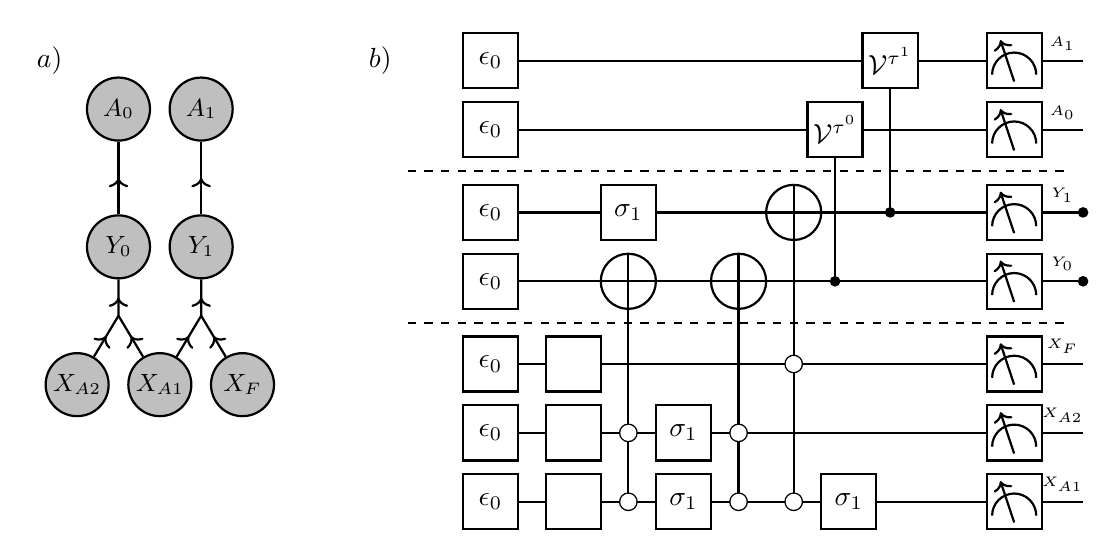
\begin{tikzpicture}[scale=0.35, thick] % , baseline = -3.5pt

            \node[anchor=center] at (-16,14) {$a)$};
            \node[anchor=center] at (-4,14) {$b)$};

            \begin{scope}[shift={(-12,2.25)}]

                \node[circle, draw, thick, fill=\nodegrayscale, minimum size = \nodeminsize] (A0) at (-1.5,10) {};
                \node[anchor=center] (A) at (-1.5,10) {\corelabelsize $\avariableof{0}$};
                \node[circle, draw, thick, fill=\nodegrayscale, minimum size = \nodeminsize] (A1) at (1.5,10) {};
                \node[anchor=center] (A) at (1.5,10) {\corelabelsize $\avariableof{1}$};

                \node[circle, draw, thick, fill=\nodegrayscale, minimum size = \nodeminsize] (H0) at (-1.5,5) {};
                \node[anchor=center] (A) at (-1.5,5) {\corelabelsize $\headvariableof{0}$};
                \node[circle, draw, thick, fill=\nodegrayscale, minimum size = \nodeminsize] (H1) at (1.5,5) {};
                \node[anchor=center] (A) at (1.5,5) {\corelabelsize $\headvariableof{1}$};

                \node[circle, draw, thick, fill=\nodegrayscale, minimum size = \nodeminsize] (F) at (3,0) {};
                \node[anchor=center] (A) at (3,0) {\corelabelsize $\catvariableof{F}$};

                \node[circle, draw, thick, fill=\nodegrayscale, minimum size = \nodeminsize] (XA1) at (0,0) {};
                \node[anchor=center] (A) at (0,0) {\corelabelsize $\catvariableof{A1}$};

                \node[circle, draw, thick, fill=\nodegrayscale, minimum size = \nodeminsize] (XA2) at (-3,0) {};
                \node[anchor=center] (A) at (-3,0) {\corelabelsize $\catvariableof{A2}$};

                \draw[->-] (H0) -- (A0);
                \draw[->-] (H1) -- (A1);

                \coordinate (F0) at (-1.5,2.5);
                \draw[->-] (XA2) -- (F0);
                \draw[->-] (XA1) -- (F0);
                \draw[->-] (F0) -- (H0);

                \coordinate (F1) at (1.5,2.5);
                \draw[->-] (F) -- (F1);
                \draw[->-] (XA1) -- (F1);
                \draw[->-] (F1) -- (H1);
            \end{scope}

            %% Ancilla Qubits

            \draw (-1,15) rectangle (1,13);
            %\node[anchor=center] (text) at (-2,14) {\colorlabelsize $\avariableof{1}$};
            \node[anchor=center] (text) at (0,14) {$\onehotmapof{0}$};
            \draw (1,14) -- (13.5,14);
            \draw (13.5,15) rectangle (15.5,13);
            \node[anchor=center] (text) at (14.5,14) {$\qcaencodingof{\hypercoreof{1}}$};
            \draw (15.5,14) -- (18,14);
            \drawqcmeasuresymbol{19}{14}
            \draw (20,14) -- (21.5,14) node[above,midway] {\colorlabelsize $\avariableof{1}$};

            \draw (14.5,8.5) -- (14.5,13);
            \drawvariabledot{14.5}{8.5}

            \draw (-1,10.5) rectangle (1,12.5);
            %\node[anchor=center] (text) at (-2,11.5) {\colorlabelsize $\avariableof{0}$};
            \node[anchor=center] (text) at (0,11.5) {$\onehotmapof{0}$};
            \draw (1,11.5) -- (11.5,11.5);
            \draw (11.5,10.5) rectangle (13.5,12.5);
            \node[anchor=center] (text) at (12.5,11.5) {$\qcaencodingof{\hypercoreof{0}}$};
            \draw (13.5,11.5) -- (18,11.5);
            \drawqcmeasuresymbol{19}{11.5}
            \draw (20,11.5) -- (21.5,11.5) node[above,midway] {\colorlabelsize $\avariableof{0}$};

            \draw (12.5,6) -- (12.5,10.5);
            \drawvariabledot{12.5}{6}

            %% Statistic Qubits
            \draw[dashed] (-3,10) -- (21,10);

            \draw (-1,7.5) rectangle (1,9.5);
            %\node[anchor=center] (text) at (-2,8.5) {\colorlabelsize $\headvariableof{1}$};
            \node[anchor=center] (text) at (0,8.5) {$\onehotmapof{0}$};
            \draw (1,8.5) -- (4,8.5);
            \draw (4,7.5) rectangle (6,9.5);
            \node[anchor=center] (text) at (5,8.5) {$\paulixsymbol$};
            \draw (6,8.5) -- (18,8.5);
            \drawcnotsymbol{11}{8.5}
            \draw (11,8.5) -- (11,-2);
            \drawqcmeasuresymbol{19}{8.5}
            \draw (20,8.5) -- (21.5,8.5) node[above,midway] {\colorlabelsize $\headvariableof{1}$};
            \drawvariabledot{21.5}{8.5}

            \draw (-1,5) rectangle (1,7);
            %\node[anchor=center] (text) at (-2,6) {\colorlabelsize $\headvariableof{0}$};
            \node[anchor=center] (text) at (0,6) {$\onehotmapof{0}$};
            \draw (1,6) -- (18,6);
            \drawcnotsymbol{9}{6}
            \draw (9,6) -- (9,-2);
            \drawqcmeasuresymbol{19}{6}
            \draw (20,6) -- (21.5,6) node[above,midway] {\colorlabelsize $\headvariableof{0}$};
            \drawvariabledot{21.5}{6}

            \drawcnotsymbol{5}{6}
            \draw (5,6) -- (5,-2);

            %% Distributed Qubits
            \draw[dashed] (-3,4.5) -- (21,4.5);

            \draw (-1,2) rectangle (1,4);
            %\node[anchor=center] (text) at (-2,3) {\colorlabelsize $\catvariableof{F}$};
            \node[anchor=center] (text) at (0,3) {$\onehotmapof{0}$};
            \draw (1,3) -- (2,3);
            \draw (2,2) rectangle (4,4);
            \node[anchor=center] (text) at (3,3) {$\hgate$};
            \draw (4,3) -- (18,3);
            \drawqcmeasuresymbol{19}{3}
            \draw (20,3) -- (21.5,3) node[above,midway] {\colorlabelsize $\catvariableof{F}$};

            \draw (-1,-0.5) rectangle (1,1.5);
            %\node[anchor=center] (text) at (-2,0.5) {\colorlabelsize $\catvariableof{A2}$};
            \node[anchor=center] (text) at (0,0.5) {$\onehotmapof{0}$};
            \draw (1,0.5) -- (2,0.5);
            \draw (2,-0.5) rectangle (4,1.5);
            \node[anchor=center] (text) at (3,0.5) {$\hgate$};
            \draw (4,0.5) -- (6,0.5);
            \draw (6,-0.5) rectangle (8,1.5);
            \node[anchor=center] at (7,0.5) {$\paulixsymbol$};

            \draw (8,0.5) -- (18,0.5);
            \drawqcmeasuresymbol{19}{0.5}
            \draw (20,0.5) -- (21.5,0.5) node[above,midway] {\colorlabelsize $\catvariableof{A2}$};

            \draw (-1,-3) rectangle (1,-1);
            %\node[anchor=center] (text) at (-2,-2) {\colorlabelsize $\catvariableof{A1}$};
            \node[anchor=center] (text) at (0,-2) {$\onehotmapof{0}$};
            \draw (1,-2) -- (2,-2);
            \draw (2,-3) rectangle (4,-1);
            \node[anchor=center] at (3,-2) {$\hgate$};
            \draw (4,-2) -- (6,-2);
            \draw (6,-3) rectangle (8,-1);
            \node[anchor=center] at (7,-2) {$\paulixsymbol$};
            \draw (8,-2) -- (12,-2);
            \draw (12,-3) rectangle (14,-1);
            \node[anchor=center] at (13,-2) {$\paulixsymbol$};
            \draw (14,-2) -- (18,-2);
            \drawqcmeasuresymbol{19}{-2}
            \draw (20,-2) -- (21.5,-2) node[above,midway] {\colorlabelsize $\catvariableof{A1}$};

            \drawcontroldot{5}{0.5}
            \drawcontroldot{5}{-2}

            \drawcontroldot{9}{0.5}
            \drawcontroldot{9}{-2}

            \drawcontroldot{11}{3}
            \drawcontroldot{11}{-2}

        \end{tikzpicture}
    \end{center}
    \caption{Circuit to sample from the \ComputationActivationNetwork{} in the toy accounting \exaref{exa:toyAccounting}.
    %Note that a first Pauli-X gate $\paulixsymbol$ acting on $\catvariableof{A2}$ can be omitted, since the prepared stated is uniform.
    }
    \label{fig:toyAccounting}
\end{figure}

\end{example}

\subsection{Acceptance Probability by $\infty$ Renyi Divergence}

In more generality we draw samples from a generic proposal distribution $\mathbb{Q}$, which support needs to include the support of the target distribution $\probtensor$.
We draw a sample $\shortcatindices$ from $\mathbb{Q}$ and accept it with the probability
\begin{align*}
    \frac{\probat{\indexedshortcatvariables}}{\mathbb{Q}\left[\indexedshortcatvariables\right]}
    \cdot \left(\max_{\shortcatindicesin}\frac{\probat{\indexedshortcatvariables}}{\mathbb{Q}\left[\indexedshortcatvariables\right]}
    \right)^{-1}
\end{align*}

The acceptance probability is the $\infty$ Renyi Divergence between the proposal distribution (typically uniform) and the target distribution.

For $0<\alpha<\infty$ and $\alpha\neq 1$ the Renyi Divergence is defined as
\begin{align*}
    D_{\alpha}\left[\probtensor||\mathbb{Q}\right]
    = \frac{1}{1-\alpha} \lnof{\sum_{\shortcatindicesin}
        \frac{\probat{\indexedshortcatvariables}^{\alpha}}{\mathbb{Q}\left[\indexedshortcatvariables\right]^{\alpha-1}}
    } \, .
\end{align*}
The $\infty$ Renyi Divergence is the limit $\alpha\rightarrow\infty$
\begin{align*}
    D_{\infty}\left[\probtensor||\mathbb{Q}\right]
    = \lnof{\max_{\shortcatindicesin}
        \frac{\probat{\indexedshortcatvariables}}{\mathbb{Q}\left[\indexedshortcatvariables\right]}
    } \, .
\end{align*}

Then we have the acceptance probability
\begin{align*}
    \secprobat{\avariable=1}
    &= \mathbb{E}_{\shortcatindices\sim\mathbb{Q}}\left[\frac{\probat{\indexedshortcatvariables}}{\mathbb{Q}\left[\indexedshortcatvariables\right]} \cdot \left(\max_{\shortcatindicesin}
                                                                                                                                                              \frac{\probat{\indexedshortcatvariables}}{\mathbb{Q}\left[\indexedshortcatvariables\right]}
    \right)^{-1}
    \right] \\
    &= \mathbb{E}_{\shortcatindices\sim\mathbb{Q}}\left[\frac{\probat{\indexedshortcatvariables}}{\mathbb{Q}\left[\indexedshortcatvariables\right]} \right] \cdot \left(\max_{\shortcatindicesin}
                                                                                                                                                                      \frac{\probat{\indexedshortcatvariables}}{\mathbb{Q}\left[\indexedshortcatvariables\right]}
    \right)^{-1} \\
    & = \left(\max_{\shortcatindicesin}
            \frac{\probat{\indexedshortcatvariables}}{\mathbb{Q}\left[\indexedshortcatvariables\right]}
    \right)^{-1}  \\
    & = \expof{-D_{\infty}\left[\probtensor||\mathbb{Q}\right]} \, .
\end{align*}

\textbf{Extension:}
We could increase the acceptance probability, when we sample from a propsal distribution $\mathbb{Q}$ with smaller $\infty$ Renyi divergence to $\probtensor$.
When sampling with Quantum Circuits, this could be implemented by a state preparation for the distributed variables, before the \ComputationActivationCircuit{} is applied.
It would be interesting to train variational quantum circuits for this task.
However, when we want to apply the same scheme as above, one needs to encode $\mathbb{Q}$ into the ancilla preparing rotations, so $\mathbb{Q}$ would need to be an elementary \ComputationActivationNetwork{} as well.

\subsection{Application}

%% Usage as forward inferer
When sampling from probability distributions, we can use these samples to estimate probabilistic queries.
Building on such particle-based inference schemes, we can perform various inference schemes for \ComputationActivationNetworks{}, such as backward inference and message passing schemes.

    \chapter{Implementation in the \tnreason{} package}\label{cha:implementation}

We here document the implementation of the discussed concepts in the \python{} package \tnreason{}, in the version \curvertnreason

% Name
\tnreason{} is an abbreviation of \textbf{t}ensor \textbf{n}etwork \textbf{reason}ing, by which we emphasize the capabilities of this package to represent and answer reasoning tasks by tensor network contractions.

% Installation
The package can be installed either by cloning the repository
\begin{center}
    \href{https://github.com/EnexaProject/enexa-tensor-reasoning}{https://github.com/EnexaProject/enexa-tensor-reasoning}
\end{center}
or by
\begin{lstlisting}
!pip install tnreason==2.0.0
\end{lstlisting}

\sect{Architecture}

\tnreason{} is structured in four subpackages and three layers
\begin{itemize}
    \item Layer 1: Storage and numerical manipulations, by subpackage \spengine{}
    \item Layer 2: Specification of workload, subpackage \sprepresentation{} specific for storage, subpackage \spreasoning{} specific for manipulations
    \item Layer 3: Applications in reasoning, by subpackage \spapplication{}
\end{itemize}

We sketch this structure by
\begin{center}
    %! Author = alexgoessmann
%! Date = 09.03.25

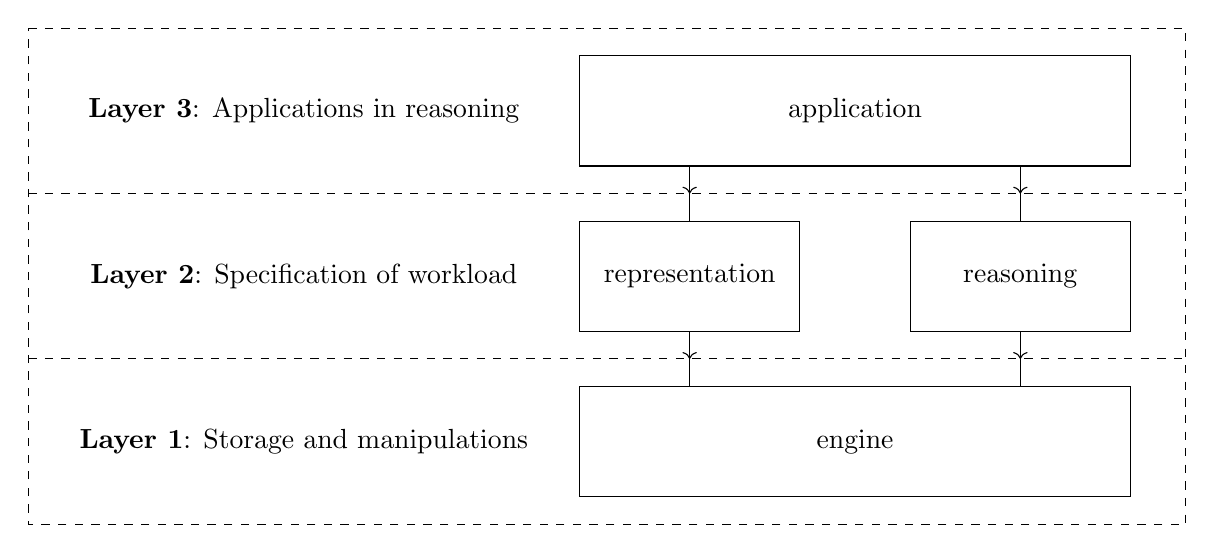
\begin{tikzpicture}[scale=0.35]
    \draw[dashed] (-30,15) -- (12,15) -- (12,-3) -- (-30,-3) -- (-30,15);

    \draw (-10,10) rectangle (10,14);
    \node [anchor=center] at (0,12) {\spapplication{}};

    \node [anchor=center] at (-20,12) {\layerthreespec};
    \draw[dashed] (-30,9) -- (12,9);
    \node [anchor=center] at (-20,6) {\layertwospec};

    \draw[->-] (6,10) -- (6,8);
    \draw (2,4) rectangle (10,8);
    \node [anchor=center] at (6,6) {\spreasoning{}};
    \draw[->-] (6,4) -- (6,2);

    \draw[->-] (-6,10) -- (-6,8);
    \draw (-10,4) rectangle (-2,8);
    \node [anchor=center] at (-6,6) {\sprepresentation{}};
    \draw[->-] (-6,4) -- (-6,2);

    \draw[dashed] (-30,3) -- (12,3);
    \node [anchor=center] at (-20,0) {\layeronespec};

    \draw (-10,-2) rectangle (10,2);
    \node [anchor=center] at (0,0) {\spengine{}};
\end{tikzpicture}
\end{center}


\sect{Implementation of basic notation}

First of all, we explain how the basis notation explained in \charef{cha:notation} is reflected in the implementation.

\subsect{\bncategoricals}
Categorical Variables are identified by strings, which then appear as colors of the corresponding tensor axes.
Their dimension is stored in shapeDicts, but most practically these shapes are stored in the tensors in which variables appear.
Suffixes in the color string (defined in \inlinecode{representation.suffixes}) denote the type of the variable:
\begin{itemize}
    \item Distributed variables with color suffix \disVarSuf: $\catvariableof{\cdot}$
    \item Computed variables with color suffix \comVarSuf: $\headvariableof{\cdot}$
    \item Selection variables with color suffix \selVarSuf: $\selvariableof{\cdot}$
    \item Term variables with color suffix \terVarSuf: $\indvariableof{\cdot}$
\end{itemize}

\subsect{\bntensors}

\paragraph{Tensors} are objects of classes inheriting \inlinecode{engine.TensorCore} with main attributes
\begin{itemize}
    \item \inlinecode{values}: Storing the coordinates of the tensors (individual realization for different cores)
    \item \inlinecode{colors}: List of the variables $[\headvariableof{\formula},\catvariableof{0},\catvariableof{1}]$
    \item \inlinecode{name}: Reflecting the notation such as $\bencodingof{\formula}$
    \item \inlinecode{shape}: Storing the dimension of each appearing variable, as a list of integers with the same length as colors.
\end{itemize}

Suffixes in the name string (defined in \inlinecode{representation.suffixes}) highlight the origin and purpose of the tensor.
Cores are named with suffixes based on their functionality
\begin{itemize}
    \item Computation core with name suffix \comCoreSuf: They represent the computation of a function in basis calculus, and are directed cores.
    Their colors are \inlinecode{[headColors] + [inputColors]}, where \inlinecode{[inputColors]} are either distributed variables or, if having a composition of formulas.
    When the function is a selection augmentation of other functions, selection colors are listed in the end of \inlinecode{[inputColors]}.
    \item Activation core with name suffix \actCoreSuf: two-dimensional vectors representing of the activation core to a formula
\end{itemize}

Both the cores and the colors are further refined by infixes before the suffices to denote specific instantiations.

\begin{itemize}
    \item \selCoreIn: Involving a selection variable
    \item \eviCoreIn: Storing evidence about a variable
    \item \heaIn: Head of a function, typically the variable computed at a activation selector
    \item \funIn: Function selection variables
    \item \posIn+\stringof{i}: Variable selection for argument at position $i$
    \item \datIn: Involving data (data cores and colors)
\end{itemize}

Further infixes are strings denoting atom names and neuron names.

Exploiting efficient representation tricks we further have the tensor name suffices:
\begin{itemize}
    \item \atoCoreSuf: Atomization core, for sparse representation of categorical constraints
    \item \vselCoreSuf: Variable selection core: For sparse representation of variable selectors
\end{itemize}

\paragraph{Initialization}
Tensors are instantiated by
\begin{lstlisting}
engine.getCore(coreType)(values, colors, name, shape)
\end{lstlisting}
where \inlinecode{coreType} is a string further specifying a specific implementation of tensors (see for more detail \secref{sec:implementationEngine}).
The default tensor implementation \defaultCoreType is chosen, when \inlinecode{coreType} is not specified.


One-hot encodings are specific tensors created in \sprepresentation{}.

\subsect{\bncontractions}

\paragraph{Tensor networks} $\tnetof{\graph}=\{\hypercoreofat{\edge}{\catvariableof{\edge}}\wcols\edge\in\edges\}$ are stored as dictionaries of tensors, where the keys coincide with the names of the corresponding tensors.
The edges of the hypergraph $\graph$ used in the definition of tensor networks in \defref{def:tensorNetwork} are here labeled by the names of the tensors and the affected variables by the list of colors, being an attribute of each tensor.

\paragraph{Contractions} are implemented in the subpackage \spengine{}, orienting on \defref{def:contraction}.
Reflected in the notation
\begin{align*}
    \contractionof{\tnetof{\graph}}{\secnodevariables}
\end{align*}
a contraction is defined by
\begin{itemize}
    \item Tensor Network $\tnetof{\graph}$, specified by a dictionary of tensor names as keys and valued by tensor cores.
    \item Open Variables $\secnodes$, specified by a list of colors to the variables.
\end{itemize}
Contraction calls are implemented as
\begin{lstlisting}
engine.contract(contractionMethod, coreDict, openColors, dimensionDict, evidenceColorDict)
\end{lstlisting}
where the arguments are
\begin{itemize}
    \item \inlinecode{contractionMethod}: str, chooses one of the contraction providers. The default contraction method \defaultContractionMethod is chosen, when
    \item \inlinecode{coreDict}: Dictionary of TensorCores (of the above formats), representing the Tensor Network $\tnetof{\graph}$
    \item \inlinecode{openColors}: List of str, each str identifying a color, that is a variable to be left open in the contraction
    \item \inlinecode{dimensionDict}: Dict valued by int and keys by str, storing dimensions to each variable. This is of optional usage, when a color in openColors does not appear in the coreDict.
    \item \inlinecode{evidenceColorDict}: Dict valued by int and keys by str, indicating sliced variables
\end{itemize}

Coordinates of tensors can be retrieved by
\begin{align*}
    \contractionof{\hypercoreat{\nodevariables}}{\secnodevariables=\catindexof{\secnodes}} \, .
\end{align*}
We implement this by leaving \inlinecode{openColors} empty and passing $\catindexof{\secnodes}$ as the \inlinecode{evidenceColorDict}, as a dictionary with keys by the \inlinecode{str} colors to the variables and values by the corresponding \inlinecode{int} indices.

Graphical illustrations can be generated by
\begin{lstlisting}
engine.draw_factor_graph(coreDict)
\end{lstlisting}
where \inlinecode{coreDict} is a tensor network to be visualized.


\subsect{\bnencoding}
Encoding schemes are implemented in the subpackage \sprepresentation{}.



\sect{Subpackage \spengine{}}\label{sec:implementationEngine}

The \spengine{} subpackage is for the storage and numerical manipulation of tensors and tensor networks.
We organize the subpackage as the lowest layer of \tnreason{}, specializing in storage of Tensor Networks and performing the contractions.

\subsect{Basis+ $\cpformat$ Decompositions storing \inlinecode{values}}

\paragraph{Specification of basis+ elementary tensors}
We orient on basis+ sparse tensor decomposition in the initialization of tensor cores, as discussed in detail in \charef{cha:sparseRepresentation}.
The basis+ elementary tensors have basis+ $\cpformat$ rank of $1$ and admit a decomposition as (see \defref{def:polynomialSparsity})
\begin{align*}
    \hypercoreat{\nodevariables}
    = \slicescalar \cdot \contractionof{\onehotmapofat{\catindexof{\variableset}}{\catvariableof{\variableset}}}{\nodevariables} \, .
\end{align*}
Elementary basis+ tensors are in \tnreason{} stored by a tuple
\begin{lstlisting}
(value, posDict)
\end{lstlisting}
where \inlinecode{posDict} specifies the values to the variables, which do not have a trivial leg vector, and \inlinecode{value} a scalar scaling the basis vector.
Comparing with the notation of \charef{cha:sparseRepresentation}, the keys of \inlinecode{posDict} correspond with $\variableset$, the values of \inlinecode{posDict} with $\catindexof{\variableset}$ and \inlinecode{value} corresponds with $\slicescalar$.

\paragraph{Elementary Iterators}
The initialization, coordinate retrieval and conversion operations of all tensor cores are oriented on basis+ $\cpformat$ Decompositions \eqref{eq:decIntoMonomials} of tensors.
A tensor
\begin{align*}
    \hypercoreat{\nodevariables}
    = \sum_{\slicetupleof{}\in\sliceset} \slicescalar \cdot \contractionof{\onehotmapofat{\catindexof{\variableset}}{\catvariableof{\variableset}}}{\nodevariables} \, .
\end{align*}
corresponds with an iterator over tuples \inlinecode{(value,posDict)}, each specifying a basis+ elementary tensor in the sum.
%Each tensor core can be iterated, where the iterations are over tuples \inlinecode{(value,posDict)} specifying a basis+ tensor.

\paragraph{Core Arithmetics}
When subscribing an instance \inlinecode{exampleCore} of \inlinecode{engine.TensorCore} by
\begin{lstlisting}
exampleCore[posDict] = value
\end{lstlisting}
a basis+ elementary tensor specified by \inlinecode{(value,posDict)} is added to its values, that is
\begin{align*}
    \hypercoreat{\shortcatvariables} \algdefsymbol \hypercoreat{\shortcatvariables} + \contractionof{\onehotmapofat{\catindexof{\variableset}}{\catvariableof{\variableset}}}{\shortcatvariables} \, .
\end{align*}
The linear structure of tensors spaces are more further reflected in sums of \inlinecode{engine.TensorCore} instances, which are implemented with the same \inlinecode{coreType}, as
\begin{lstlisting}
summed = exampleCore1 + exampleCore2
\end{lstlisting}
and scalar multiplication, where a scalar \inlinecode{value} of type \inlinecode{int} or \inlinecode{float}
\begin{lstlisting}
multiplied = value * exampleCore
\end{lstlisting}
Both operations are performed as manipulations of the tensors \inlinecode{values}.
Contraction of two \inlinecode{engine.TensorCore} instances are performed by
\begin{lstlisting}
contracted = exampleCore1.contract_with(exampleCore2)
\end{lstlisting}
and are used in corewise contraction, where \inlinecode{contractionMethod="CorewiseContractor"}.

\paragraph{Initialization}
Any instance of \inlinecode{engine.TensorCore} is initialized as a vanishing tensor $\onesat{\nodevariables}$, when \inlinecode{values} is not specified.
The values are then assigned by iteration over a \inlinecode{sliceIterator} over \inlinecode{(value,posDict)} tuples specifying elementary basis+ tensors, where the $\cpformat$ rank is the length of the iterator
%A basis+ $\cpformat$ tensor is specified by an iterator \inlinecode{sliceIterator} over elementary basis+ tensors, where the $\cpformat$ rank is the length of the iterator
This initialization is by applied in the method
\begin{lstlisting}
engine.create_from_slice_iterator(shape, colors, sliceIterator, coreType, name)
\end{lstlisting}
where \inlinecode{shape, colors, coreType, name} are used in the call of an empty core by \\
\inlinecode{engine.get_core} and \inlinecode{sliceIterator} used to iterative add the basis+ elementary tensors to create the tensor.

\paragraph{Storage of basis+ $\cpformat$ decompositions}
The implemented tensor classes derived from \\
\inlinecode{engine.TensorCore} differ in their implementation of \inlinecode{values}.
Motivated from basis+ $\cpformat$ decompositions, most classes rely on a data base storing the \inlinecode{(value,posDict)} tuples.
An overview over the derived classes is provided in \figref{tab:tensorClasses}.
Here \inlinecode{PandasCore}, \inlinecode{TentrisCore} and \inlinecode{PolynomialCore} support sparse basis+ $\cpformat$ decompositions, by utilizing \inlinecode{pandas.DataFrame}, \inlinecode{tentris.hypertrie} and \inlinecode{list} as storage data base.
These are implementations of the matrix representation of \remref{rem:matStorageBasPlus}.
The \inlinecode{NumpyCore} class on the other hand is based relies on arrays as \inlinecode{numpy.array} as storage solution, which corresponds with the demand that each \inlinecode{posDict} contains all colors of the tensor.
Effectively, this amounts to restricting to basis $\cpformat$ decomposition, which demanded ranks are always larger than basis+ $\cpformat$ decompositions (see \theref{the:rankCascade}).

\begin{figure}
    \begin{center}
        \begin{tabular}{|c|c|c|c|}
            \hline
            \textbf{coreType}           & \textbf{Used Package}                       & \text{Storage of \inlinecode{values}}             & \textbf{Sparse basis+ $\cpformat$ support} \\
            \hline
            \inlinecode{NumpyCore}      & \inlinecode{numpy}                          & \inlinecode{numpy.array}                          & No                                         \\
            \hline
            \inlinecode{PandasCore}     & \inlinecode{pandas}                         & \inlinecode{pandas.DataFrame}                     & Yes                                        \\
            \hline
            \inlinecode{TentrisCore}    & \inlinecode{tentris}  \cite{bigerl_tentris_2020} & \inlinecode{tentris.hypertrie} & Yes\\
            \hline
            \inlinecode{PolynomialCore} & $--$                                        & \inlinecode{list} of \inlinecode{(value,posDict)} & Yes\\
            \hline
        \end{tabular}
    \end{center}
    \caption{Derived classes from \inlinecode{engine.TensorCore}, differing in the implemented storage of \inlinecode{values}.}\label{tab:tensorClasses}
\end{figure}




\subsect{Contractions}

%\textbf{Binary CP Decomposition}
%
%Based on the monomial decomposition $\polsparsityof{\cdot}$ as specified in \defref{def:polynomialSparsity}.
%To store the values of a tensor we store the slices of tensors by the indices $\catindexof{\variableset}$.
%
%% Trick -> To BinaryCP
%Contractions can be performed by partially contracting the cores of the decomposition.
%In this way, one can avoids coordinatewise storages of high-order tensors, which can be intractable.


% Contraction Method List
The supported contraction methods are listed in \figref{tab:contractionMethods}.

\begin{figure}
    \begin{center}
        \begin{tabular}{|p{\threecolumnwidth}|p{\threecolumnwidth}|p{\threecolumnwidth}|}
            \hline
            \textbf{contractionMethod} (str)   & \textbf{Package}                            & \textbf{Applied procedure}                                \\
            \hline
            \stringof{NumpyEinsum}             & \inlinecode{numpy}                          & Einstein summation \inlinecode{numpy.einsum}              \\
%        \hline
%        \stringof{TensorFlowEinsum}        & $\mathrm{tensorflow}$ & Einstein summation of $\mathrm{tensorflow}$ tensors         \\
%        \hline
%        \stringof{TorchEinsum}             & $\mathrm{torch}$      & Einstein summation of $\mathrm{torch}$ tensors              \\
            %\hline
            \stringof{TentrisEinsum}           & \inlinecode{tentris}  \cite{bigerl_tentris_2020} & Einstein summation \inlinecode{tentris.einsum}            \\
            %\hline
            \stringof{PgmpyVariableEliminator} & \inlinecode{pgmpy}                          & Variable Elimination of \inlinecode{pgmpy.DiscreteFactor} \\
            %\hline
            \stringof{CorewiseContractor}      & $--$                                        & Contraction using \inlinecode{core.contract_with()}       \\
            \hline
        \end{tabular}
    \end{center}
    \caption{Implemented contraction methods in \tnreason{}.}
    \label{tab:contractionMethods}
\end{figure}

\paragraph{Einstein Summation}
is a syntax of specifying the contractions of arrays.
Different possibilities are available to optimize over possible contraction paths, for example in \inlinecode{numpy} by the \inlinecode{numpy.einsum_path}.
%Contractions represented as Einstein summation, as implemented in:
%\begin{itemize}
%	\item numpy
%	\item tensorflow
%	\item pytorch
%	\item tentris
%\end{itemize}

\paragraph{Variable Elimination}
contracts along a junction tree, build by variable elimination.
We here use an implementation in the \inlinecode{pgmpy} package.

\paragraph{Corewise Contraction}
uses the \inlinecode{contract_with} method of tensor cores to contract in a given order.





\sect{Subpackage \sprepresentation{}}\label{sec:implementationRepresentation}

The \sprepresentation{} subpackage consists in a collection of core creation methods.
%Here the basis encodings $\bencodingof{\exfunction}$ of various maps $\exfunction$ are created.
We arrange the \sprepresentation{} subpackage into the second layer of the \tnreason{} architecture, since it specifies tensor cores which formats are specified in \spengine{}.

\paragraph{Coordinate Calculus}
Coordinatewise transformations (see \defref{def:coordinatewiseTransform}) are supported by
\begin{lstlisting}
engine.coordinatewise_transform(coresList, transformFunction)
\end{lstlisting}
where \inlinecode{coresList} is a list of $\seldim$ tensors with identical variables and \inlinecode{transformFunction} a function $\chainingfunction: \parspace \rightarrow \rr$.

\paragraph{Basis Calculus}
Basis encodings (see \defref{def:functionRelationEncoding}) of functions $\exfunction:\facstates \rightarrow \secfacstates$ are created by
\begin{lstlisting}
engine.create_relational_encoding_from_lambda(inshape, outshape, incolors, outcolors, indicesToIndices)
\end{lstlisting}
where \inlinecode{indicesToIndices} is a lambda-function representing $\exfunction$ and \inlinecode{inshape, outshape, incolors, outcolors} specify the input and output variables.
Let us notice, that this procedure produces sums of $\facdim$ basis tensors corresponding with a basis $\cpformat$ decompositions.
More involved initialization procedures based on basis+ elementary tensors calling \\
\inlinecode{engine.create_from_iterator} might result in sparser representations.

\paragraph{Propositional Connectives} are represented by strings.
\figref{tab:connectives} lists the supported logical connectives, which are implemented in \inlinecode{representation.basisplus_calculus}.
If the \inlinecode{str} to the connective starts with \stringof{n}, then the negated connective is encoded.

\begin{figure}
    \begin{center}
        \begin{tabular}{|p{\fivecolumnwidth}|p{\fivecolumnwidth}|p{\threecolumnwidth}|p{\fivecolumnwidth}|p{\fivecolumnwidth}|}
            \hline
            \textbf{$\exconnective$}          & \textbf{$\synencodingof{\exconnective}$} & \textbf{Notes} & $\baspluscprankof{\exconnective}$ & $\baspluscprankof{\bencodingof{\exconnective}}$ \\
            \hline
            $\land$                           & \stringof{and}                           &                                                                   & 1                                 & 3                                               \\
            %\hline
            $\lor$                            & \stringof{or}                            &                                                                   & 2                                 & 3                                               \\
            %\hline
            $\Rightarrow$                     & \stringof{imp}                           & last variable as head, others premises                            & 2                                 & 3                                               \\
            %\hline
            $\oplus$                          & \stringof{xor}                           & implemented as the negation of \stringof{eq}, i.e. \stringof{neq} & 3 & 5 \\
            %\hline
            $\Leftrightarrow$                 & \stringof{eq}                            &                                                                   & 2                                 & 5                                               \\
            %\hline
            $\catvariableof{\atomenumerator}$ & \stringof{pas} + "$\atomenumerator$"     & $\atomenumerator$th atom & 1 & 2 \\
            %\hline
            $\lnot$                           & \stringof{not}                           & negation of the first argument, i.e. \stringof{npas0}             & 1                                 & 2                                               \\
            \hline
        \end{tabular}
    \end{center}
    \caption{Supported connectives in the script language.
    The arity of all connectives is not restricted.
    We notice that the basis+ rank $\baspluscprankof{\bencodingof{\exconnective}}$ is independent of the arity and in most cases less than the naive bound of $2^{\catorder}$.
    }\label{tab:connectives}
\end{figure}


% WOLFRAM Numbers

\paragraph{Wolfram codes} provide a classification scheme of propositional formuals by natural numbers, which is supported in the script language.
%They provide a generic representation scheme of propositional formulas by the so-called
The Wolfram code has been designed for the classification of cellular automaton rules \cite{wolfram_statistical_1983} and popularized in the book \cite{wolfram_new_2002}.
Along this, the coordinate encodings of $\catorder$-ary connectives $\exconnective$ are flattened and interpreted as a binary number, which is transformed into a decimal number and represented as a string $\synencodingof{\exconnective}$.
To be more precise, to each $\catorder$-ary connective its Wolfram code is calculated by
\begin{align*}
    N(\exconnective) = \sum_{\catindex\in[2^\catorder]} 2^{2^{\catorder}-\catindex-1} \cdot \exconnective(\catindex) \, .
\end{align*}
In the script language, the connective is represented by the string concatenation of the arity and the Wolfram code as
\begin{align*}
    \synencodingof{\exconnective} = "\catorder" + "_" + "N(\exconnective)" \, .
\end{align*}

\subsect{Computation Activation Networks}

\paragraph{Features} are generation procedures of activation cores given canonical parameters.
They are initialized by
\begin{lstlisting}
ComputedFeature(featureColors, affectedComputationCores, shape, name)
\end{lstlisting}
where
\begin{itemize}
    \item \inlinecode{featureColors} is a list of \inlinecode{str} variable colors, which are assigned to a created activation core
    \item \inlinecode{affectedComputationCores} is a list of \inlinecode{str} names of computation cores, which are required to compute the feature colors
    \item \inlinecode{shape} is a list of \inlinecode{int} dimensions to the variables
\end{itemize}
Mean parameters to features are computed by
\begin{lstlisting}
exampleFeature.compute_meanParam(environmentMean)
\end{lstlisting}
where \inlinecode{environmentMean} is the contraction of a tensor network with open colors by the \\
\inlinecode{featureColors}.
They are further capable of computing local changes to canonical parameter in order to match mean parameters by
\begin{lstlisting}
exampleFeature.local_update(environmentMean, meanParam)
\end{lstlisting}
To customize their purposes, individual feature classes are derived from \\
\inlinecode{representation.ComputedFeature}, as listed in \figref{tab:featureTypes}.

\begin{figure}
    \begin{center}
        \begin{tabular}{|p{\fourcolumnwidth}|p{\fourcolumnwidth}|p{\fourcolumnwidth}|p{\fourcolumnwidth}|}
            \hline
            \textbf{featureType} & \textbf{Purpose} & \textbf{Canonical Parameter} & \textbf{Activation Core} \\
            \hline
            \stringof{SingleSoftFeature} & $\sstatcoordinateof{\selindex}$ of a statistic
            & Scalar (\inlinecode{int} or \inlinecode{float})  & $\expof{\canparam \cdot \indexinterpretationofat{\imageof{\sstatcoordinateof{\selindex}}}{\headvariableof{\selindex}}}$           \\
            \hline
            \stringof{SoftPartitionFeature} & Partition statistics (see \defref{def:partitionStatistic}) $\sstat$ %(Boolean statistic $\sstat$ such that $\contractionof{\sencsstat}{\nodevariables}=\onesat{\nodevariables}$
            & $\canparamat{\selvariable}$  & $\expof{\canparamat{\selvariable}}$   \\
            \hline
            \stringof{HardPartitionFeature} & Partition statistics (see \defref{def:partitionStatistic})
            & Boolean tensor $\canparamat{\selvariable}$  & $\canparamat{\selvariable}$ \\
            \hline
        \end{tabular}
    \end{center}
    \caption{Features derived from \inlinecode{representation.ComputedFeature}, which are implemented in \inlinecode{representation.features}.}
    \label{tab:featureTypes}
\end{figure}

\paragraph{Computation Activation Networks} are the most general models representable in \tnreason{}.
They generalize distributions such as those computable by a statistic (see \defref{def:realizableStatDistributions}) as well as constraint satisfaction problems (see \defref{def:csp}).
Computation Activation Networks are initialized by
\begin{lstlisting}
representation.ComputationActivationNetwork(featureDict, computationCoreDict, baseMeasureCoreDict, canParamDict)
\end{lstlisting}
where
\begin{itemize}
    \item \inlinecode{featureDict} is a dictionary of features, where the keys correspond with the names of the features
    \item \inlinecode{computationCoreDict} is a tensor network of computation cores, which needs to contain all names of computation cores required to compute all feature colors
    \item \inlinecode{baseMeasureCoreDict} is a tensor network representing of $\basemeasureat{\nodevariables}$
    \item \inlinecode{canParamDict} is a dictionary of canonical parameters (see \figref{tab:featureTypes})
\end{itemize}
Computation Activation Networks can be instantiated as cores by \\
\inlinecode{exampleCANetwork.create_cores()} or as an energy dictionary by \\
\inlinecode{exampleCANetwork.get_energy_dict()}.
Energy dictionaries are stored as dictionaries with values by tuples \inlinecode{value, tensorNetwork}, representing a by \inlinecode{value} weighted sum of the \inlinecode{tensorNetwork}.

\begin{example}[Representation of a member of an exponential family]\label{exa:expFamilyCARep}
    To represent $\expdistof{\sstat,\canparam,\basemeasure}$ we initialize a
    \begin{itemize}
        \item \inlinecode{featureDict} as a dictionary of \inlinecode{representation.SingleSoftFeature} to each feature $\sstatcoordinateof{\selindex}$
        \item \inlinecode{computationCoreDict} $\extnet$ of computation cores such that
        \begin{align*}
            \extnetat{\headvariables,\nodevariables} = \bencodingofat{\sstat}{\headvariables,\nodevariables} \, .
        \end{align*}
        Decompositions and redundancies between coordinates $\sstatcoordinateof{\selindex}$ can be exploited to find an efficient tensor network.
        \item \inlinecode{baseMeasureCoreDict} $\secextnet$ to represent the base measure $\basemeasure$
        \item \inlinecode{canParamDict} of canonical parameters, valued by the coordinates $\canparamat{\indexedselvariable}$
    \end{itemize}
\end{example}



\sect{Subpackage \spreasoning{}}\label{sec:implementationReasoning}


The \spreasoning{} subpackage implements contraction-based reasoning algorithm on representation.ComputationActivationNetworks.
%basic tensor network algorithms with calls of specific execution in \spengine{}.
As the \sprepresentation{} subpackage it is arranged in the second layer of the \tnreason{} architecture, since it specifies the manipulation of tensor networks in the \spengine{} subpackage.

\subsect{Sampling}

Sampling is performed by MCMC methods calling local sampling methods, which are derived classes from \inlinecode{reasoning.SampleCoreBase}.

The energy-based algorithms execute reasoning tasks solely on energy dictionaries, which are created by \inlinecode{representation.ComputationActivationNetwork.get_energy_dict()}.
\begin{lstlisting}
reasoning.EnergyBasedGibbs
\end{lstlisting}


\subsect{Variational Inference}
An overview over the variational inference methods in presented in \figref{tab:inferenceMethods}.

\paragraph{Forward mappings} are implemented by \inlinecode{reasoning.ForwardContractor} as contraction of all cores, and in \inlinecode{reasoning.ExpectationPropagator} as a message-passing approach.

\paragraph{Backward mappings} (see \secref{sec:backwardMap}) are implemented by \inlinecode{reasoning.BackwardAlternator} as alternating algorithms iteratively updating the canonical parameters to single features (see \algoref{alg:AMM}).

\paragraph{Mean field methods} are approximation methods of energy tensors by tractable exponential families (see \secref{sec:meanField}).
Given an energy dictionary the naive mean field method is implemented as %(e.g. created by \inlinecode{exampleCANetwork.get_energy_dict()})
\begin{lstlisting}
reasoning.NaiveMeanField(energyDict)
\end{lstlisting}
and the more general markov network based mean field method by
\begin{lstlisting}
reasoning.GenericMeanField(energyDict, edgeColorDict)
\end{lstlisting}
where \inlinecode{edgeColorDict} specifies the graph of the approximating markov network.


\begin{figure}
    \begin{center}
        \begin{tabular}{|p{\threecolumnwidth}|p{\threecolumnwidth}|p{\threecolumnwidth}|}
            \hline
            \textbf{inferenceMethod} (str)   & \textbf{Applied procedure}                               & \textbf{Dependency}                                               \\
            \hline
            \stringof{ForwardContractor}     & Contraction of all cores keeping the feature colors open  & $--$\\
            %\hline
            \stringof{BackwardAlternator}    & Iterative local updates to match the mean parameters & Forward inferer to iteratively update the mean parameters \\
            %\hline
            \stringof{ExpectationPropagator} & Iterative updates of messages between feature clusters & Forward and backward inferer used for the computation of messages \\
            \hline
        \end{tabular}
    \end{center}
    \caption{Implemented inference methods in \tnreason{}.}
    \label{tab:inferenceMethods}
\end{figure}



\subsect{Optimization}

Optimization is a reasoning task of finding a maximal coordinate given a tensor network.
The supported methods are implemented in \inlinecode{reasoning.optimization_handling} and listed in \figref{tab:optimizationMethods}.

\begin{figure}
    \begin{center}
        \begin{tabular}{|p{\threecolumnwidth}|p{\threecolumnwidth}|p{\threecolumnwidth}|}
            \hline
            \textbf{optimizationMethod} (str) & \textbf{Package}      & \textbf{Applied procedure}                                                 \\
            \hline
            \stringof{numpyArgMax}            & \inlinecode{numpy}    & Transformation into a numpy core and solution by \inlinecode{numpy.argmax} \\
            %\hline
            \stringof{gurobi}                 & \inlinecode{gurobipy} & Transformation into an ILP and solution by \inlinecode{gurobipy.optimize}  \\
            %\hline
            \stringof{gibbsSample}            & $--$                  & Simulated annealing based on gibbs sampling                                \\
            %\hline
            \stringof{meanFieldSample}        & $--$                  & Mean field approximation combined with \stringof{gibbsSample}              \\
            \hline
        \end{tabular}
    \end{center}
    \caption{Implemented optimization methods in \tnreason{}.}
    \label{tab:optimizationMethods}
\end{figure}



\sect{Subpackage \spapplication{}}\label{sec:implementationApplication}

With the \spapplication{} subpackage we provide an interface for reasoning workload.
It builds a third layer, since it used \sprepresentation{} to represent knowledge by tensor networks and \spreasoning{} in the execution of reasoning tasks.
%
A user-friendly high-level syntax of script language (logical formulas or neuro-symbolic architectures) for the specification of tensor networks creation, such as propositional formulas or categorical constraints, is introduced.
Given a specification of a formula $\exformula$ in script language $\synencodingof{\cdot}$, the task amounts to building a semantic representation based on the syntactic specification.


\subsect{Representation of formulas}

Propositional formulas $\exformula$ are represented in three schemes:
\begin{itemize}
    \item Syntactical representation by a script language $\synencodingof{\exformula}$ as nested lists (see \secref{subsec:scriptLanguage}).
    %Most practical to choose a formula from a neuro-symbolic architecture.
    \item Syntactical representation by a \inlinecode{str} specifying a color to the categorical variables $\headvariableof{\exformula}$.
    \item Representation of formulas by tensor networks being contracted to $\bencodingofat{\exformula}{\headvariableof{\exformula},\nodevariables}$
\end{itemize}

Conversions of the formats:
\begin{itemize}
    \item $\synencodingof{\exformula}$ to color by
    \begin{lstlisting}
application.get_formula_color(S(f))
    \end{lstlisting}
    Here the nested lists are turned in a string by concatenating all elements of a list with \stringof{\_} and adding \stringof{[} and \stringof{]} at the beginning and end of each list.
    \item  $\synencodingof{\exformula}$ to tensor network
    \begin{lstlisting}
application.create_raw_cores(S(f))
    \end{lstlisting}
    This creates the connective cores for the semantic representation of $\bencodingof{\exformula}$.
    We encode them by iterative calls of \inlinecode{engine.create_from_iterators}.
\end{itemize}

%When encoding formulas with hard interpretation, we furthermore add a head core of type \stringof{truthEvaluation} since we have
%\[ {\exformula} = \contractionof{\bencodingof{\exformula},\tbasis}{\catvariableof{\exformula}} \, . \]

\subsect{Script Language}\label{subsec:scriptLanguage}

To specify propositional sentences, neuro-symbolic architectures and \MarkovLogicNetworks{}, we developed a script language.

% Atoms

\paragraph{Atomic Formulas} are represented by arbitrary strings, which are not used for the representation of connectives.
We further avoid the symbols \{\stringof{(}, \stringof{)}, \stringof{\_}\} in the names of atoms, to not confuse them with colors of categorical variables.

% Composed Formulas

\paragraph{Composed Formulas} are represented by nested lists, where each sublist is either specifying an atomic formula (if string) or another composed formula.
For example, a formula $\exformula_1\exconnective,\exformula_2$ is represented by
\begin{centeredscript}
    $\synencodingof{\exformula_1\exconnective,\exformula_2}$ = [$\synencodingof{\exconnective}$, $\synencodingof{\exformula_1}$, $\synencodingof{\exformula_2}$]
\end{centeredscript}
where we apply the conventions
\begin{itemize}
    \item Connectives are at the 0th position in each list
    \item Further entries are either atoms as strings or encoded formulas itself
\end{itemize}
The nested lists follows a grammar, which is provided in \figref{tab:bnFunctions} in its Backus-Naur form.


% Backus-Naur
\begin{figure}
    \begin{center}
        \begin{tabular}{|p{2cm}|p{8cm}|}
            %\hline
            %Unary Connective  & \stringof{not} | \stringof{id}                                                  \\
            \hline
            $\atomorder$-ary connective & \stringof{and} | \stringof{or} | \stringof{imp} | \stringof{xor}  | \stringof{eq} | \stringof{not} | $\cdots$ \\
            & \stringof{\atomorder} + "$\_$" + \stringof{N}, where $N<2^{2^{\atomorder}-1}$                               \\
            \hline
            Atomic Formula              & Set of strings not in Connectives                                                                           \\
            \hline
            Complex Formula             & Atomic Formula | [$\atomorder$-ary connective, $\atomorder$ Complex Formulas]                               \\
            %& [Binary Connective, Complex Formula, Complex Formula]                           \\
            \hline
        \end{tabular}
    \end{center}
    \caption{Backus-Naur form of the grammar producing the nested list expressions.
    The string connectives are either appearing in the list of \figref{tab:connectives}, or represented by a Wolfram code.
    }\label{tab:bnFunctions}
\end{figure}



\begin{example}[Encoding of the Wet Street example]
    For example we have
    \begin{itemize}
        \item
        Atomic variable $\var{Rained}$ by
        \begin{centeredscript}
            $\synencodingof{\var{Rained}}$
			= \stringof{Rained}
        \end{centeredscript}
        \item
        Negative literal $\lnot\var{Rained}$ by
        \begin{centeredscript}
            $\synencodingof{\lnot\var{Rained}}$
			= [\stringof{not},\stringof{Rained}]
        \end{centeredscript}
        \item
        Horn clause $\left(\var{Rained}\Rightarrow\var{Wet}\right)$ by
        \begin{centeredscript}
            $\synencodingof{\var{Rained}\Rightarrow\var{Wet}}$
			= [\stringof{imp},\stringof{Rained},\stringof{Wet}]
        \end{centeredscript}
        \item
        Knowledge Base
        $(\lnot\var{Rained})\land(\var{Rained}\Rightarrow\var{Wet})$ by
        \begin{centeredscript}
            $\synencodingof{\lnot\var{Rained})\land(\var{Rained}\Rightarrow\var{Wet}}$
			=  [\stringof{and}, [\stringof{not}, \stringof{Rained}], [\stringof{imp}, \stringof{Rained}, \stringof{Wet}]]
        \end{centeredscript}
    \end{itemize}
\end{example}




\textbf{Knowledge Bases}

% Should distinguish these in knowledge?
We distinguish here formulas, with propositional logic interpretation and formulas which have a soft logic interpretation.
%\textbf{Facts.}
The formulas with hard interpretation are called facts in a knowledge base $\kb$ and encoded by dictionaries
\begin{centeredscript}
    \{key($\exformula$) : $\synencodingof{\exformula}$ for $\exformula\in\kb$ \}
\end{centeredscript}

\textbf{\MarkovLogicNetworks{}}

%\textbf{Weighted formulas.}
The formulas with soft interpretation are called weighted formulas and encoded by $\expof{\weightof{\exformula}\cdot\exformula}$.
We thus require a specification of the weights, which we do by adding $\weightof{\exformula}$ as a $\mathrm{float}$ or an $\mathrm{int}$ to the list $\synencodingof{\exformula}$.
We then store \MarkovLogicNetworks{} by dictionaries
\begin{centeredscript}
    \{key($\exformula$) : $\synencodingof{\exformula}$ + [$\weightof{\exformula}$] for $\exformula\in\formulaset$\}
\end{centeredscript}

\textbf{Neuro-Symbolic Architecture by Nested Lists}

% Generalizing the script language to specify architectures
To specify neuro-symbolic architectures in terms of formula selecting maps, as has been the subject of \charef{cha:formulaSelection} we further exploit the nested list structure of encoding propositional logics.
We replace, in each hierarchy of the nested structure each entry by a list of possible choices.
In this way, we reinterpret the list index as the choice indices $\selindex$ introduced for connective and formula selections (see \defref{def:connectiveSelector} and \ref{def:formulaSelector}).
More formally, the production rules are formalized in \figref{tab:bnNeurons} by the extension of the Backus-Naur form in \figref{tab:bnFunctions}.

% Neurons
\paragraph{Connective selectors} (see \defref{def:connectiveSelector}) are encoded by the list
\begin{centeredscript}
    $\synencodingof{\exconnective}$
			= [$\synencodingof{\exconnective_{0}}$, $\ldots$, $\synencodingof{\exconnective_{\seldim\shortminus1}}$]
\end{centeredscript}
and a formula selector (see \defref{def:formulaSelector}) by
\begin{centeredscript}
    $\synencodingof{\fselectionmap}$
			= [$\synencodingof{\exconnective_{0}}$, $\ldots$, $\synencodingof{\exconnective_{\seldim\shortminus1}}$]
\end{centeredscript}

\paragraph{A logical neuron} of order $\selorder$ (see \defref{def:fsNeuron}), defined by a connective selector $\exconnective$, and a formula selector $\fselectionmap_\atomenumerator$ on each argument $\atomenumerator\in[\selorder]$, is encoded by
\begin{centeredscript}
    $\synencodingof{\lneuron}$
			= [$\synencodingof{\exconnective}$, $\synencodingof{\fselectionmap_0}$, $\ldots$,  $\synencodingof{\fselectionmap_{\selorder-1}}$]
\end{centeredscript}
Only the unary $\selorder=1$ and the $\selorder=2$ cases are supported.


% Confusing?
The resulting nested lists indices have an alternating interpretation at each level compared with the elements of each list.
That is, when $\synencodingof{\lneuron}$ is the encoding of a neuron, then any element $x\in\synencodingof{\lneuron}$ represents a list of choices.
When $x$ is not the first element, then each choice is either the encoding $\synencodingof{\catvariable}$ of an atomic formula, or another neuron.

% Find another symbol?

\paragraph{A neural architecture} $\larchitecture$ is then represented in the dictionary
\begin{centeredscript}
    $\synencodingof{\larchitecture}$ = \{key($\lneuron$) : $\synencodingof{\lneuron}$ for $\exformula\in\larchitecture$\}
\end{centeredscript}
%To store this structure, we choose dictionaries of neuron spe
%\begin{centeredscript}
%	\{key($\lneuron$) : $\synencodingof{\lneuron}$ for $\exformula\in\formulaset$\}
%\end{centeredscript}
where key($\lneuron$) is a string, which can be used in the formula selections of other neurons.

% Important for well-definedness
It is important that the directed graph of neurons induced by the choice possibilities is acyclic, to ensure a well-defined architecture.


\begin{figure}
    \begin{center}
        \begin{tabular}{|p{2cm}|p{8cm}|}
            %\hline
            %Unary Connectives  & [Unary Connective] | [Unary Connective] + Unary Connectives    \\
            \hline
            $\atomorder$-ary connectives & [$\atomorder$-ary connective] | [$\atomorder$-ary connective] + $\atomorder$-ary connectives \\
            %\hline
            %Neuron Name & Any set of strings not used for atoms or connectives \\
            \hline
            Dependency Choice            & Atomic Formula | Neuron                                                                      \\
            \hline
            Dependency Choices           & [Dependency Choice] | [Dependency Choice] + Dependency Choices                               \\
            \hline
            Neuron                       & [$\atomorder$-ary connectives, $\atomorder$ Dependency Choices]                              \\
            % & [Binary Connectives, Dependency Choices, Dependency Choices]   \\
            \hline
        \end{tabular}
    \end{center}
    \caption{Extension of the grammar in Backus-Naur form in \figref{tab:bnFunctions} to describe selections of functions.}\label{tab:bnNeurons}
\end{figure}


\begin{example}[Neuro-Symbolic Architecture for the Wet Street]
    Following the wet street example, we can define a neuron by
    \begin{centeredscript}
        $\synencodingof{\lneuron}$ = [[\stringof{imp},\stringof{eq}],[\stringof{Wet},\stringof{Sprinkler}],[\stringof{Street}]]
    \end{centeredscript}
    from which the formulas
    \begin{centeredscript}
        [\stringof{imp}, \stringof{Wet}, \stringof{Street}] \\
		\hspace{0.25cm} [\stringof{eq}, \stringof{Wet}, \stringof{Street}] \\
		\hspace{1cm}[\stringof{imp}, \stringof{Sprinkler}, \stringof{Street}] \\
		\hspace{1cm}[\stringof{eq}, \stringof{Sprinkler}, \stringof{Street}]
    \end{centeredscript}
    can be chosen.
    Combining this neuron with further neurons, e.g. by the architecture
    \begin{centeredscript}
        $\synencodingof{\larchitecture}$ = \{ \stringof{neur1}: [[\stringof{imp},\stringof{eq}],[\stringof{neur2}],[\stringof{Street}]] , \\
		\hspace{1.8cm}\stringof{neur2}: [[\stringof{lnot},\stringof{id}],[\stringof{Wet},\stringof{Sprinkler}],[\stringof{Street}]] \}
    \end{centeredscript}
    the expressitivity increases.
    In this case, the further neuron provides the flexibility of the first atoms to be replaced by its negation.
\end{example}



\subsect{Distributions}

%\paragraph{}
%We encode Markov Networks by specifying a set of tensor cores.
Distributions are procedures to specify \inlinecode{representation.ComputationActivationNetworks} and are derived from the base class \inlinecode{representation.DistributionBase}.
Each distribution needs to have a routine
\begin{lstlisting}
exampleDistribution.create_caNetwork()
\end{lstlisting}
creating the corresponding network.
%creating the factor cores and
%\begin{lstlisting}%
%	.get_partition_function()
%\end{lstlisting}
%calculating the partition function.
%Although the partition function can be calculated by the contraction of all cores, we separate the method since there are situations where a faster calculation can be performed.

\paragraph{Markov Networks} are distributions, which do not have computation cores.
The positive coordinates of the factors are represented by \inlinecode{representation.SoftPartitionFactors} and the support of the factors \inlinecode{representation.HardPartitionFactors}.
%\begin{lstlisting}
%	application.
%\end{lstlisting}

\paragraph{Empirical Distributions} are special instances of Markov Networks specifying distributions of sample data.
We represent the values as a $\cpformat$ Format of data cores as specified in \secref{sec:empDistribution}.
They are initialized by
\begin{lstlisting}
application.get_empirical_distribution(sampleDf, atomColumns, interpretation, dimensionsDict)
\end{lstlisting}
where
\begin{itemize}
    \item \inlinecode{sampleDf} is a \inlinecode{pandas.DataFrame} specifying the data
    \item \inlinecode{atomColumns} is a list of column names in \inlinecode{sampleDf} to be extracted as variables of the distribution.
    \item \inlinecode{interpretation} is either \stringof{atomic} or \stringof{categorical}, specifying whether the entries in \inlinecode{sampleDf} are interpreted as uncertainties in the interval $[0,1]$, or as assignments to
\end{itemize}

Here the partition function is the number of samples used in the creation of the empirical distribution.


\textbf{HybridKnowledgeBases} are probability distributions, which are specified by propositional formulas in the script language.
\begin{lstlisting}
application.HybridKnowledgeBase
\end{lstlisting}
They are initialized with arguments
\begin{itemize}
    \item facts: Dictionary of propositional formulas stored as $\synencodingof{\exformula}$ representing hard logical constraints
    \item weightedFormulas: Dictionary of propositional formulas stored as $\synencodingof{\exformula}$+$[\weightof{\exformula}]$ representing soft logical constraints
    \item evidence: Dictionary of atomic formulas, where key are the formulas in string representation and values the certainty in $[0,1]$ (float or int) of the atom being true
    \item categoricalConstraints: Dictionary of categorical constrained, which values are lists of atomic formulas stored as strings $\synencodingof{\atomicformula}$
\end{itemize}


\subsect{Inference}

To simplify deductive inference on models a class
\begin{lstlisting}
application.InferenceProvider
\end{lstlisting}
taking a \inlinecode{representation.ComputationActivationNetwork} or \inlinecode{application.Distribution} has been implemented.

% Probabilistic Queries

\paragraph{Probabilistic queries} as specified \defref{def:queries})  by
\begin{lstlisting}
.query(variableList, evidenceDict)
\end{lstlisting}

\paragraph{Mode queries} by
\begin{lstlisting}
.exact_map_query()
\end{lstlisting}
%or by
%\begin{lstlisting}
%	.annealed_sample()
%\end{lstlisting}
%using Simulated Annealing (see Remark~\ref{rem:simulatedAnnealing}) to find an approximate maximum.
%The second method circumvents the creation of the coordinatewise representation of the distribution and circumvents therefore, at the expense of potentially approximative solutions, a bottleneck in case of many query variables.

% Entailment Queries

\paragraph{Entailment} from the distribution (\defref{def:probEntailment}) is be decided by
\begin{lstlisting}
.ask(queryFormula, evidenceDict)
\end{lstlisting}
where queryFormula is the formula $\exformula$ to be tested for entailment in the representation $\synencodingof{\exformula}$.

% Sampling

\paragraph{Samples} can be drawn by
\begin{lstlisting}
.draw_samples(sampleNum, variableList, annealingPattern)
\end{lstlisting}
based on Gibbs sampling, where
\begin{itemize}
    \item sampleNum (int) gives the number of samples to be drawn
    \item variableList (list of str) defines the variables to be represented by the samples (default: all atoms in the distribution)
    \item annealingPattern specifies an annealing pattern
\end{itemize}


%\subsect{Parameter Estimation}
%
%\textbf{EntropyMaximizer} implements Algorithm~\ref{alg:AWO}, which is motivated by the maximum entropy principle (see \secref{sec:maxEntProblem}) to optimize \MarkovLogicNetworks{}.
%The class
%\begin{lstlisting}
%	application.EntropyMaximizer
%\end{lstlisting}
%is initialized with the arguments
%\begin{itemize}
%    \item expressionsDict: Dictionary of formulas in the format $\synencodingof{\exformula}$
%    \item satisfactionDict: Dictionary of the satisfaction rates (mean parameters) to be matched by the optimal distribution
%\end{itemize}
%The optimization is then performed by
%\begin{lstlisting}
%	.alternating_optimization(sweepNum, updateKeys)
%\end{lstlisting}
%method, where the iteration in  through the updateKeys is performed sweepNum times.

\subsect{Learning}

To learn instances of \inlinecode{application.HybridKnowledegBase} on data the class
\begin{lstlisting}
application.HybridLearner
\end{lstlisting}
is initialized with the arguments
\begin{itemize}
    \item knowledgeBase: Distribution representing a current model to be improved
    \item specDict: A neuro-symbolic architecture encoded in a dictionary of neurons
\end{itemize}

\paragraph{Formula Selecting Neural Networks} (\defref{def:fsNeuron})
are specified to define a proposal distribution.
They are encoded by creating all formula selecting neurons, each involving a
\begin{itemize}
    \item a connective selection map (\defref{def:connectiveSelector})
    \item variable selection cores (\defref{def:variableSelector}) to each argument using the decomposition of \theref{the:varSelectorDecomposition}.
\end{itemize}
Each selection variable of each neuron comes with a control variable with suffix \stringof{\_sV}.

\paragraph{Structure Learning}
is performed by
\begin{lstlisting}
application.HybridLearner.propose_candidate()
\end{lstlisting}
where a proposal distribution is instantiated and then sampled given the specified inference method.

\paragraph{Weight Estimation}
is performed by
\begin{lstlisting}
application.HybridLearner.infer_weights_on_data(empDistribution)
\end{lstlisting}
where \inlinecode{empDistribution} is used to infer the mean parameters to be matched by the canonical parameters of \inlinecode{knowledgeBase.weightedFormulas}.

    \appendix


    \section{Extension: Sampling from proposal distributions}

    We can prepare basis circuit encodings to selection augmented formulas, in this way introducing formula selecting networks.

    \textbf{Idea for an inductive reasoning scheme:} Prepare a q-sample from the empirical distribution and the current distribution.
    Then prepare the basis circuit encodings, where the selection variables are shared and the distributed variables assigned to the prepared samples.
    Now, the ancilla qubits can be designed to $\onehotmapof{1}$ and $\onehotmapof{0}$ accordingly.
    The rejection sampling scheme on both ancillas being $1$ and the measurement of $\selvariable$ prepares then the distribution
    \begin{align*}
        \normalizationof{
            \contractionof{\empdistributionwith, \sencmlnstatwith}{\selvariable}, \contractionof{\currentdistributionwith}{\selvariable}
        }{\selvariable}
    \end{align*}
    That is, the probability of selecting $\selindex$ is proportional to
    \begin{align*}
        \datameanat{\indexedselvariable} \cdot (1-\currentmeanat{\indexedselvariable})
    \end{align*}
    and thus prefers formulas, which have a large empirical mean, but a small current mean.

    \textbf{Open Question:} Since the distribution is "similar" to $\expof{\datameanat{\indexedselvariable}-\currentmeanat{\indexedselvariable})}$ (terms appear in Taylor of first order), can we tune the distribution with an inverse temperature parameter $\beta$?


    \section{Comparing tensor networks and quantum circuits}

    First of all, we need to extend to complex tensors, which are maps
    \begin{align*}
        \hypercore : \atomstates \rightarrow \mathbb{C} \,
    \end{align*}
    with image in $\mathbb{C}$ instead of $\mathbb{R}$ as in the report.

    A coarse comparison of the nomenclature used for quantum circuits and tensor networks:

    \begin{center}
        \begin{tabular}{l|l}
            \textbf{Quantum Circuit} & \textbf{Tensor Network}   \\
            \hline
            Qubit                    & Boolean Variable          \\
            Quantum Gate             & Unitary Tensor            \\
            Quantum Circuit          & Tensor Network on a graph
        \end{tabular}
    \end{center}

    Some constraints appear for a tensor network to be a quantum circuit
    \begin{itemize}
        \item \textbf{Unitarity of each gate:} That is the variables of each tensor are bipartite into sets $\variablesetof{\insymbol}$ and $\variablesetof{\outsymbol}$ of same cardinality and the basis encoding with respect to this bipartition, that is
        \begin{align*}
            T_{\insymbol \rightarrow \outsymbol}[\catvariableof{\insymbol},\catvariableof{\outsymbol}] : \bigotimes_{\atomenumerator\in\variablesetof{\insymbol}} \mathbb{C}^2 \rightarrow \bigotimes_{\atomenumerator\in\variablesetof{\outsymbol}} \mathbb{C}^2  \, ,
        \end{align*}
        is a unitary map, that is
        \begin{align*}
            \left(T_{\insymbol \rightarrow \outsymbol}\right)^H \circ \left(T_{\insymbol \rightarrow \outsymbol}\right)
            = \contractionof{
                T_{\insymbol \rightarrow \outsymbol}[\catvariableof{\insymbol},\seccatvariable],
                \overline{T}_{\insymbol \rightarrow \outsymbol}[\seccatvariable,\catvariableof{\outsymbol}]
            }{\catvariableof{\outsymbol},\catvariableof{\insymbol}}
            = \identityat{\catvariableof{\outsymbol},\catvariableof{\insymbol}}.
        \end{align*}
        \item \textbf{Incoming-Outgoing structure:} Variable appear at most once as incoming and at most once as outgoing variables.
        Those not appearing as outgoing (respectively as incoming) are the input and the output variables of the whole circuit.
        \item \textbf{Acyclicity:} Incoming and outgoing variables of each tensor core provide a direction of each edge tensor. With respect to this directionality the graph underlying the tensor network has to be acyclic.
    \end{itemize}

    The unitary tensors can be aligned layerwise, if and only if the last two assumption hold, i.e. the directed graph is acyclic and each variable appears at most once as an incoming and at most once as an outgoing variable.


    \section{POVM measurements as contractions}

    The main difficulty of using quantum circuits as contraction providers is that we can only extract information through measurements.
    Therefore measurement is the only way to execute contractions of the circuit, which come with restrictions when interested in contraction with open variables.

    The most general measurement formalism is through a POVM, a set $\{E_\seccatindex \, : \, \seccatindex\in[r]\}$ of positive operators with % Nielsen book notation
    \begin{align*}
        \sum_{\seccatindex\in[r]} E_\seccatindex = I
    \end{align*}

    Measuring a pure state $\ket{\psi}$ We then get outcome $m$ with probability
    \begin{align*}
        \braket{\psi|E_\seccatindex|\psi}
    \end{align*}

    We define a measurement variable $\headvariable$ taking indices $\seccatindex\in[r]$ and a measurement tensor
    \begin{align*}
        E[\headvariable,\catvariableof{\insymbol},\catvariableof{\outsymbol}]
    \end{align*}
    with slices
    \begin{align*}
        E[\headvariable=\seccatindex,\catvariableof{\insymbol},\catvariableof{\outsymbol}] = E_\seccatindex \, .
    \end{align*}

    Repeating the measurement asymptotically on a state $\ket{\psi}$ prepared by a quantum circuit $\tnetof{\graph}$ acting on the trivial start state $\ones$, we denote the measurement outcome by $\seccatindex^\datindex$.
    In the limit $\datanum\rightarrow\infty$ we get almost surely
%    we thus get the contraction
    \begin{align*}
        \frac{1}{\datanum} \sum_{\datindexin} \onehotmapofat{\seccatindex^\datindex}{\headvariable} \rightarrow
        \contractionof{\tnetof{\graph}[\catvariableof{\insymbol}],E[\headvariable,\catvariableof{\insymbol},\catvariableof{\outsymbol}],\tnetof{\secgraph}[\catvariableof{\outsymbol}]}{\headvariable} \, .
    \end{align*}

    % Case of computational basis measurements
    POVMs to computational basis measurements of subsets of qubits are constructed as products with delta tensors on the non-measured qubits.


    \section{Alternative Contraction Provider: Overlap-measuring Circuits}

    Quantum Circuits such as the SWAP test and the Hadamard test can be used to measure overlaps of quantum states, which are the squared absolutes of contractions of two state tensors.
    \begin{itemize}
        \item When we have preparation schemes for two tensors, we can control them with a common ancilla qubit and measure their contraction by a Hadamard test (alternatively, using the SWAP test and state preparation in two registers).
        \item Can we extend these schemes to contractions of more general tensor networks?
    \end{itemize}

    \bibliographystyle{plainnat}
    \bibliography{../../references.bib}


\end{document}